%% 
%% Copyright 2019-2024 Elsevier Ltd
%% 
%% Version 2.4
%% 
%% This file is part of the 'CAS Bundle'.
%% --------------------------------------
%% 
%% It may be distributed under the conditions of the LaTeX Project Public
%% License, either version 1.2 of this license or (at your option) any
%% later version.  The latest version of this license is in
%%    http://www.latex-project.org/lppl.txt
%% and version 1.2 or later is part of all distributions of LaTeX
%% version 1999/12/01 or later.
%% 
%% The list of all files belonging to the 'CAS Bundle' is
%% given in the file `manifest.txt'.
%% 
%% Template article for cas-dc documentclass for 
%% double column output.

%\documentclass[a4paper,fleqn,longmktitle]{cas-dc}
\documentclass[a4paper,fleqn]{cas-dc}

\usepackage[T1]{fontenc}
\usepackage[utf8]{inputenc}
\usepackage[numbers]{natbib}
\setcitestyle{numbers,sort,open={[},close={]},citesep={],[}}
\usepackage{subfig}
\usepackage{rotating}

\hypersetup{citecolor=blue,linkcolor=blue,urlcolor=blue}


%%%Author definitions
\def\tsc#1{\csdef{#1}{\textsc{\lowercase{#1}}\xspace}}
\tsc{WGM}
\tsc{QE}
\tsc{EP}
\tsc{PMS}
\tsc{BEC}
\tsc{DE}
%%%

\begin{document}

% ========== Title Page ==========
%\thispagestyle{empty}
%\begin{center}
%{\Large\bfseries TITLE PAGE}
%\end{center}

%\vspace{0.8cm}

%\begin{center}
%{\Large\bfseries ChainOptNet: An intelligent multi-level learning framework for adaptive blockchain system performance optimization}
%\end{center}

%\vspace{1cm}

%\noindent\textbf{First Author: Jun Liu}\\
%\textbf{\textit{Affiliation:}} School of Computer Science and Technology, Chongqing University of Posts and Telecommunications, Chongqing 400065\\
%City: Chongqing\\
%State: Chongqing\\
%Country: China\\
%Email: liujun@cqupt.edu.cn

%\vspace{0.6cm}

%\noindent\textbf{Second Author: Bin Shi}\\
%\textbf{\textit{Affiliation:}} School of Computer Science and Technology, Chongqing University of Posts and Telecommunications, Chongqing 400065\\
%City: Chongqing\\
%State: Chongqing\\
%Country: China\\
%\textbf{Email:} shibin4252@163.com

%\vspace{0.6cm}

%\noindent\textbf{Third Author: Mingwei Lin}\\
%\textbf{\textit{Affiliation:}} College of Computer and Cyber Security, Fujian Normal University, Fuzhou, Fujian 350117\\
%City: Fuzhou\\
%State: Fujian\\
%Country: China\\
%Email:linmwcs@163.com

%\vspace{0.6cm}

%\noindent\textbf{Fourth Author: Jianting Ning}\\
%\textbf{\textit{Affiliation:}} College of Computer and Cyber Security, Fujian Normal University, Fuzhou, Fujian 350117\\
%City: Fuzhou\\
%State: Fujian\\
%Country: China\\
%Email: jtning88@gmail.com

%\vspace{0.6cm}

%\noindent\textbf{Fifth Author: Meikang Qiu}\\
%\textbf{\textit{Affiliation:}} School of Computer and Cyber Sciences, Augusta University\\
%City: Augusta\\
%State: Georgia\\
%Country: USA\\
%Email: qiumeikang@yahoo.com

%\vspace{0.8cm}

%\noindent\textbf{Corresponding Author:} Jun Liu, Mingwei Lin\\
%\textbf{Corresponding Author Email:} liujun@cqupt.edu.cn, linmwcs@163.com\\
%\textbf{Corresponding Author Telephone:} +86 13996377550, +86 15980668595 (Mingwei Lin)\\
%Address: Chongqing 400065\\
%City: Chongqing\\
%State: Chongqing\\
%Country: China



%\clearpage
% ========== End Title Page ==========

%	\let\WriteBookmarks\relax
%	\def\floatpagepagefraction{1}
%	\def\textpagefraction{.001}
%	\shortauthors{Jun Liu et~al.}
	
	% 标题部分
	\title[mode = title]{ChainOptNet: An intelligent multi-level learning framework for adaptive blockchain system performance optimization}
	
	% 基金脚注
	%\tnotetext[1]{This work was supported by the Chongqing Research Program of Basic Research and Frontier Technology (Grant No. CSTB2025NSCQ-GPX1309).}
	
	% ========== 作者定义 ==========
%	\author[1]{Jun Liu}
%	\cormark[1]
%	\ead{liujun@cqupt.edu.cn}
	
%	\author[1]{Bin Shi}
%	\ead{shibin4252@163.com}
	
%	\author[2]{Mingwei Lin}
%	\cormark[1]
%	\ead{linmwcs@163.com}
	
%	\author[2]{Jianting Ning}
%	\ead{jtning88@gmail.com}
	
%	\author[3]{Meikang Qiu}
%	\ead{qiumeikang@yahoo.com}
	
	% 单位信息
%	\affiliation[1]{organization={School of Computer Science and Technology, Chongqing University of Posts and Telecommunications},
%		city={Chongqing},
%		postcode={400065}, 
%		country={China}}
	
%	\affiliation[2]{organization={College of Computer and Cyber Security, Fujian Normal University},
%		city={Fuzhou},
%		postcode={350117}, 
%		country={China}}
	
%	\affiliation[3]{organization={School of Computer and Cyber Sciences, Augusta University},
%		city={Augusta},
%		state={Georgia},
%		postcode={30902},
%		country={USA}}
	
	% 通讯作者标注
%	\cortext[cor1]{Corresponding authors: Jun Liu (liujun@cqupt.edu.cn), Mingwei Lin (linmwcs@163.com)}
	\begin{abstract}
		Blockchain has emerged as a transformative technology with numerous applications due to its tamper-proof, traceable, and decentralized architecture. Nonetheless, its performance remains constrained, particularly in areas such as latency and throughput, which pose significant barriers to large-scale deployment. This paper proposes ChainOptNet, a novel blockchain system performance optimization framework that addresses these challenges with three key technical contributions. First, we develop the Convolutional Feature Aggregation and Distribution (CFAD) model to forecast transaction arrival rates. This model uses a deep learning architecture to capture transaction data's temporal dependencies and complex statistical patterns. Second, we present a multi-model collaborative framework for blockchain performance prediction that improves predictive accuracy and robustness by intelligently integrating diverse machine learning models. Third, we create a Dynamic Weight Deep Q-Network (DW-DQN) optimization mechanism that combines a DQN-based block-size controller with a trend-aware dynamic reward weighting module for balanced multi-objective optimization. 
		Experimental evaluations show that CFAD achieves the lowest MAE and RMSE at all three evaluated time intervals, while the performance prediction ensemble achieves the lowest MAPE for both latency and throughput. The optimization module also reduces average latency and increases average throughput relative to the evaluated fixed block-size configurations.
		The reported latency optimization rate reaches 50.73\% relative to a fixed block size of 100, while the reported throughput optimization rate reaches 22.09\% relative to a fixed block size of 50. These results demonstrate the framework’s scalability, adaptability, and strong potential for practical deployment in diverse blockchain environments.
	\end{abstract}
	
	
	
	\begin{keywords}
		Blockchain system \sep Performance optimization \sep Transaction arrival rate prediction \sep Deep reinforcement learning \sep Machine learning \sep Block size adjustment
	\end{keywords}
	
	\maketitle
	
\section{Introduction}

Blockchain technology has quickly evolved into a transformative paradigm across multiple domains, providing decentralized, tamper-resistant, and transparent solutions for data exchange and transaction processing \citep{10824862},\citep{akanfe2024blockchain},\citep{jie2023secure},\citep{lin2024computing}. Its fundamental properties, which include immutability, traceability \citep{huang2025blockchain},\citep{zhang2023secure}, and consensus-driven trust \citep{xu2023survey}, have enabled widespread adoption in fields such as digital finance \citep{gan2024trust},\citep{javaid2022review}, supply chain management \citep{chen2021bidm},\citep{cui2023dschain}, healthcare \citep{ramzan2022healthcare}, the Internet of Things (IoT) \citep{gaiblock2022blockchain},\citep{gai2019privacy},\citep{huang2022blocksense},\citep{el2024ddos}, and smart grids \citep{deebak2022lightweight},\citep{wang2019energy},\citep{zhou2019secure},\citep{khoa2024collaborative}.



Despite these benefits, blockchain systems still face significant performance bottlenecks, particularly in terms of scalability \citep{park2024watchdog},\citep{choi2023lmpt},\citep{liu2021hypermaze}. Existing public blockchains, such as Bitcoin and Ethereum, have limited transaction processing capabilities, averaging around 7 and 30 transactions per second (TPS), respectively \citep{nakamoto2008bitcoin},\citep{buterin2013ethereum}. These rates fall far short of the requirements for high-throughput applications, such as financial exchanges and IoT networks \citep{begum2022systematic},\citep{ni2022novel},\citep{an2024rlchain}. In addition, the latency required for transaction confirmation can range from a few seconds to minutes, making blockchain unsuitable for latency-sensitive services like real-time payments or industrial automation \citep{chen2019collaborative},\citep{yang2022blockchain},\citep{liao2024rt}. These limitations are exacerbated by dynamic workloads, in which transaction arrival rates and network conditions (such as node participation and network latency) fluctuate unpredictably as a result of external user behavior or system-level events. In such cases, traditional blockchain configurations, which are statically defined at the time of deployment, lack the responsiveness required to adapt to real-time changes. This causes to increased block propagation delays, transaction congestion, and inefficient resource utilization. Moreover, practical blockchain deployments are often affected by fluctuating node participation, heterogeneous hardware capabilities, and geographically distributed network infrastructures. These factors introduce varying communication delays and resource availability, further complicating performance optimization. Therefore, an effective optimization framework should continuously adapt to workload evolution while maintaining stable performance under changing network conditions.



To address these performance issues, researchers have proposed a number of improvement strategies. Alternative consensus algorithms such as Proof-of-Stake (PoS) and Practical Byzantine Fault Tolerance (PBFT), aim to reduce consensus latency and increase throughput \citep{xu2023adaptchain},\citep{gao2021sharding},\citep{zhang2021trustworthy},\citep{dai2024wahoo}, but they frequently compromise decentralization and scalability. Some approaches use heuristic or rule-based tuning of system parameters, such as adjusting block size or gas limits based on network statistics \citep{chen2023decision},\citep{monem2024sustainable},\citep{jamil2022improving},\citep{chen2022latency},\citep{wilhelmi2022end}. Some researchers have also introduced machine learning-based methods for tuning blockchain parameters \citep{wang2022bpr}, with the goal of optimizing performance in a more adaptive and data-driven manner. Recently, some researchers have used performance scoring mechanisms to dynamically optimize blockchain configuration parameters \citep{wang2023learningchain}. These methods can effectively supplement and synergize with existing efforts, providing a promising path to improving blockchain performance.


However, these strategies typically lack adaptability and robustness because they rely on manually defined thresholds that may be insufficient under unpredictable or changing conditions. Furthermore, while machine learning methods provide more flexibility, the accuracy of the proposed performance prediction models can still be improved, and their scalability is frequently limited by high training data requirements, which may result in additional data collection and computational costs. Furthermore, while advances such as improved consensus algorithms and blockchain sharding have demonstrated potential in controlled environments \citep{xu2023adaptchain},\citep{li2023lb}, their practical implementation frequently encounters significant technical barriers and intricate customization requirements. These include the varying complexity of real-world application scenarios and the diverse needs of blockchain users, which limit the solutions' universal applicability. Notably, recent scoring-based optimization methods \citep{wang2023learningchain} also face challenges such as static weight configurations, limited real-time adaptability, manually defined tuning rules, limited deployment scope, and inadequate handling of multi-objective trade-offs. These limitations reduce their effectiveness in dynamic and heterogeneous blockchain environments. Overall, most existing methods are constrained by rigid architectures or fixed policies, which significantly reduces their effectiveness in rapidly changing operational environments.



To address the aforementioned limitations, we introduce ChainOptNet, a unified and adaptive blockchain performance optimization framework that integrates key processes, such as transaction arrival rate prediction, performance forecasting, and dynamic parameter tuning. In contrast to existing methods that handle these tasks in isolation, ChainOptNet uses a tightly coupled design that allows for real-time adaptation to dynamic network environments. The framework achieves high responsiveness and robustness by systematically coordinating learning-based components. Extensive evaluations across a variety of blockchain scenarios show consistent improvements in throughput and latency over representative baselines from forecasting, regression, ensemble-learning, and score-based optimization categories, highlighting its strong adaptability and scalability in complex environments. The primary contributions of this paper are summarized as follows:

\begin{itemize}
	\item We introduce CFAD, a convolutional sequence model designed to capture complex nonlinear temporal dependencies found in blockchain transaction patterns. CFAD allows for accurate short-term and mid-term forecasting of transaction arrival rates, which serves as a crucial input for downstream optimization.
	
	\item We propose a collaborative multi-model performance prediction framework that includes heterogeneous learning models. The framework improves forecasting robustness across different performance indicators by using inverse error-weighted ensemble learning, even when the historical data is noisy or incomplete.
	
	\item We present DW-DQN, a reinforcement learning-based optimization module with a trend-aware dynamic reward weighting mechanism. The DQN learns the block-size adjustment policy, while the reward weights for latency and throughput are deterministically computed from recent performance trends, enabling efficient multi-objective trade-offs in dynamic network environments.
	
	\item We run extensive experiments across a wide range of blockchain scenarios to validate ChainOptNet's superior performance, adaptability, and scalability under varying workloads and network conditions. The findings show that ChainOptNet can learn effective parameter adjustment strategies by leveraging temporal patterns, ensemble learning, and dynamic reward tuning, demonstrating ChainOptNet's effectiveness and superiority for blockchain system performance optimization.
\end{itemize}



The remainder of this paper is organized as follows. Section~\ref{sec:related} reviews related work on blockchain performance prediction and optimization. Section~\ref{sec:motivation} presents the motivation for this study. Section~\ref{sec:system} presents the architecture and operational design of ChainOptNet. Section~\ref{sec:experiments} details the experimental setup and presents comparative analyses.   Section~\ref{sec:conclusion} concludes the paper and discusses future research directions.




\section{Related work}\label{sec:related}

As blockchain technology becomes increasingly widespread across various applications, performance issues such as low throughput and high latency have emerged as major bottlenecks. Existing research has explored a range of optimization strategies from different perspectives to address these challenges.

Recent studies have also explored transaction conflict management and ledger design. \citet{wu2026fabrictca} proposed FabricTCA, which improves Hyperledger Fabric throughput by mitigating intra-block and inter-block transaction conflicts. \citet{ma2026mixchain} introduced MixChain, an Account-Vessel hybrid ledger model that reduces transaction dependencies to facilitate parallel execution. These approaches improve blockchain performance through changes to transaction processing and ledger architecture, whereas ChainOptNet focuses on adaptive block-size adjustment.

\subsection{Improvement of consensus algorithms}
\vspace{6pt}
Improving the consensus mechanism is one of the most common approaches to enhancing blockchain performance. \citet{gao2021sharding} proposed a piecewise hash graph consensus algorithm designed for industrial IoT, which significantly improves throughput and reduces latency. \citet{zhang2021trustworthy} enhanced the performance of Hyperledger Fabric by modifying its consensus module, thereby achieving a better trade-off between security and efficiency. \citet{xu2023adaptchain} introduced AdaptChain, an elastic blockchain that supports adaptive expansion and contraction based on transaction volume, optimizing resource utilization while maintaining high performance.
\citet{li2024secure} proposed a hybrid consensus mechanism that integrates intra-shard processing with lightweight global coordination, addressing the issues of vulnerable consensus security and delayed atomicity in cross-shard transactions while maintaining adaptive shard management.
\citet{islam2025proof} proposed Proof of Random Leader (PoRL), a PoA-based consensus algorithm that employs verifiable random functions to enhance throughput and ensure fair leader selection, thus addressing the limitations of low throughput and predictable leader rotation in existing PoA variants such as Aura and Clique.

\subsection{Blockchain sharding}
\vspace{6pt}
Sharding techniques partition the blockchain network into multiple shards to enhance parallelism and scalability. \citet{cai2022benzene} developed Benzene, a collaboration-based sharding system that improves throughput while maintaining shard-level security. \citet{li2023lb} presented LBChain, a load-balancing sharding scheme that dynamically migrates accounts among shards based on activity levels, effectively balancing transaction loads and boosting throughput.
\citet{yang2024ezchain} introduced EZchain, a passive sharding protocol that achieves constant communication and storage costs without requiring cross-shard transactions or beacon chains, offering improved scalability and security in large networks.
\citet{liu2023flexible} proposed a flexible sharding (FS) blockchain protocol that features cross-shard Byzantine fault tolerance (CSBFT) to reduce confirmation delays, multiple parallel CSBFT to enhance system parallelism, and decentralized shard reconfiguration. This effectively addresses key challenges in cross-shard transaction processing and security vulnerabilities.
\citet{jia2024estuary} proposed a low cross-shard protocol, which features a multi-level state model and a community overlap propagation algorithm to dramatically reduce cross-shard transactions.
The X-shard system \citep{xu2024x} addresses cross-shard processing bottlenecks through transaction pattern-based allocation and optimistic parallel processing, achieving near-linear throughput scaling and reduced latency.

\subsection{Optimization based on traditional algorithms}
\vspace{6pt}
Several studies have employed classical optimization algorithms to fine-tune blockchain parameters. \citet{jamil2022improving} applied Particle Swarm Optimization (PSO) to evaluate the trade-off between throughput and latency in Hyperledger Fabric, aiming to determine the optimal transaction arrival rate. \citet{chen2022latency} deployed a private Ethereum IoT network and used probabilistic fitting to model its latency performance. \citet{wilhelmi2022end} utilized Markov Chains to determine the optimal block size configuration for minimizing latency through numerical analysis.

\subsection{Machine learning-based optimization}
\vspace{6pt}
Recent advances have introduced machine learning (ML) to predict system behavior and support intelligent decision-making in blockchain environments. \citet{wang2022bpr} proposed a performance prediction framework that employs Multilayer Perceptron (MLP) and Long Short-Term Memory (LSTM) networks to predict blockchain performance and transaction arrival rates. However, this approach does not address issues such as the cost of collecting blockchain performance data, its generalization capability under small sample sizes, and the integration of predictive modeling with system-level optimization. Other prediction-driven optimization methods combine temporal workload forecasting, performance prediction, and score-based configuration adjustment to improve throughput and latency \citep{wang2023learningchain}. Although these methods provide a more flexible alternative to manual tuning, they often depend on predefined scoring functions or fixed decision rules, making it difficult to adapt the optimization objective when latency and throughput priorities change across operating regimes.


Reinforcement learning has also been applied to permissioned blockchain optimization. \citet{tang2026enhancing} proposed Rail-Fabric, a framework for low-latency movement authority generation in train control systems. The framework uses a Double Deep Q-Network (DDQN) to dynamically partition the railway network and adjust sub-blockchain boundaries. While Rail-Fabric focuses on topology-aware partitioning, ChainOptNet combines workload forecasting and performance prediction with block-size control and trend-aware reward weighting.

%\subsection{Research Motivation}

%Despite significant progress in blockchain performance optimization, several key limitations remain unaddressed:

%\begin{itemize}
	%\item Disjoint optimization stages: Most existing approaches treat workload prediction and system-level optimization as separate processes. This decoupling can result in suboptimal configuration strategies, especially in rapidly changing environments.
	
	%\item Limited generalization of ML models: Machine learning-based methods often rely on extensive and balanced datasets to perform accurately. In blockchain networks, however, available data can be sparse, imbalanced, or noisy, which severely impacts the generalizability and robustness of predictive models.
	
	%\item Lack of adaptability: Many existing optimization techniques rely on static parameters or fixed rules, making them poorly suited to dynamic blockchain environments where transaction loads and network conditions vary unpredictably over time.
	
	%\item Real-time decision-making challenges: Current frameworks often lack mechanisms for real-time adjustment based on streaming inputs, resulting in delayed reactions to sudden workload surges or network degradations.
%\end{itemize}

%These gaps highlight the need for an integrated, data-driven, and adaptive optimization framework that can operate effectively under dynamic and heterogeneous blockchain conditions.


%Although the aforementioned studies have achieved promising results, a number of limitations remain:
%(1) Workload prediction and system optimization are often addressed separately, resulting in suboptimal configurations;
%(2) Machine learning models struggle to generate effective results under limited or imbalanced blockchain data, especially in dynamic environments;
%(3) Current approaches often use static optimization strategies that lack adaptability to fluctuating network conditions and do not support real-time data.

%To fill these gaps, this paper proposes ChainOptNet, a unified blockchain performance optimization framework that includes: (i) a deep learning-based transaction arrival rate prediction model (CFAD), (ii) a multi-model ensemble for performance forecasting, and (iii) a dynamic weight reinforcement learning strategy (DW-DQN) for real-time block size adjustment. Table~\ref{tab:comparison} includes a detailed comparison of existing methods to our proposed framework.

\section{Research motivation}\label{sec:motivation}

This section identifies key limitations in current blockchain optimization: the disjoint handling of workload prediction and system tuning, the poor generalization of machine learning models under data scarcity and noise, and the lack of adaptability and real-time responsiveness in dynamic environments.

\subsection{Disjoint optimization and lack of adaptability in dynamic environments}
\vspace{6pt}
Current blockchain optimization strategies often treat transaction workload prediction and system-level configuration separately, and many of them use static configurations or rule-based policies, assuming stable environments \citep{jamil2022improving},\citep{chen2022latency},\citep{wilhelmi2022end},\citep{wang2022bpr},\citep{wang2023learningchain},\citep{leng2019manuchain}. In dynamic blockchain environments, transaction arrival rates fluctuate unpredictably due to user behavior or external events, and node participation and transaction volumes are also volatile. Without tight integration between prediction and control, and without adaptive strategies that can autonomously update configurations in response to observed changes, workload predictions cannot effectively guide proactive adjustments to system parameters like block size or gas limit, leading to inefficient resource allocation, increased latency, and poor performance under shifting workloads.

\subsection{Limited generalization under data constraints}
\vspace{6pt}
Machine learning–based blockchain performance prediction often relies on abundant, high-quality training data, which is rarely available in real-world deployments. Public blockchains may have imbalanced datasets, while consortium blockchains often suffer from small sample sizes \citep{marsalek2019tackling}. Additionally, blockchain data is frequently noisy due to inconsistent node behaviors or heterogeneous network conditions, challenging learning algorithms and limiting model generalization \citep{xu2017information}. A robust framework must incorporate models resilient to such data deficiencies.


\subsection{Summary}
\vspace{6pt}
To address these gaps, this paper proposes ChainOptNet, a unified blockchain performance optimization framework featuring: (i) a deep learning–based transaction arrival rate prediction model (CFAD), (ii) a multi-model ensemble for performance prediction, and (iii) a dynamic weight reinforcement learning strategy (DW-DQN) for real-time block size adjustment. 
%Table~\ref{tab:comparison} compares existing methods with the proposed framework.


\section{System model}\label{sec:system}
\subsection{Overall framework}
\vspace{6pt}

Figure~\ref{fig:overallframe} depicts the proposed ChainOptNet framework for blockchain performance optimization, which dynamically adjusts the block size according to real-time network conditions and historical transaction information. The framework takes historical transaction arrival rates together with blockchain configuration parameters, including block size, the number of ordering nodes, latency, and throughput, as inputs, and outputs the optimal block size to improve overall blockchain performance. As illustrated in Fig.~\ref{fig:overallframe}, the proposed framework consists of the following three components:

\begin{figure*}[thbp]
	\centering
	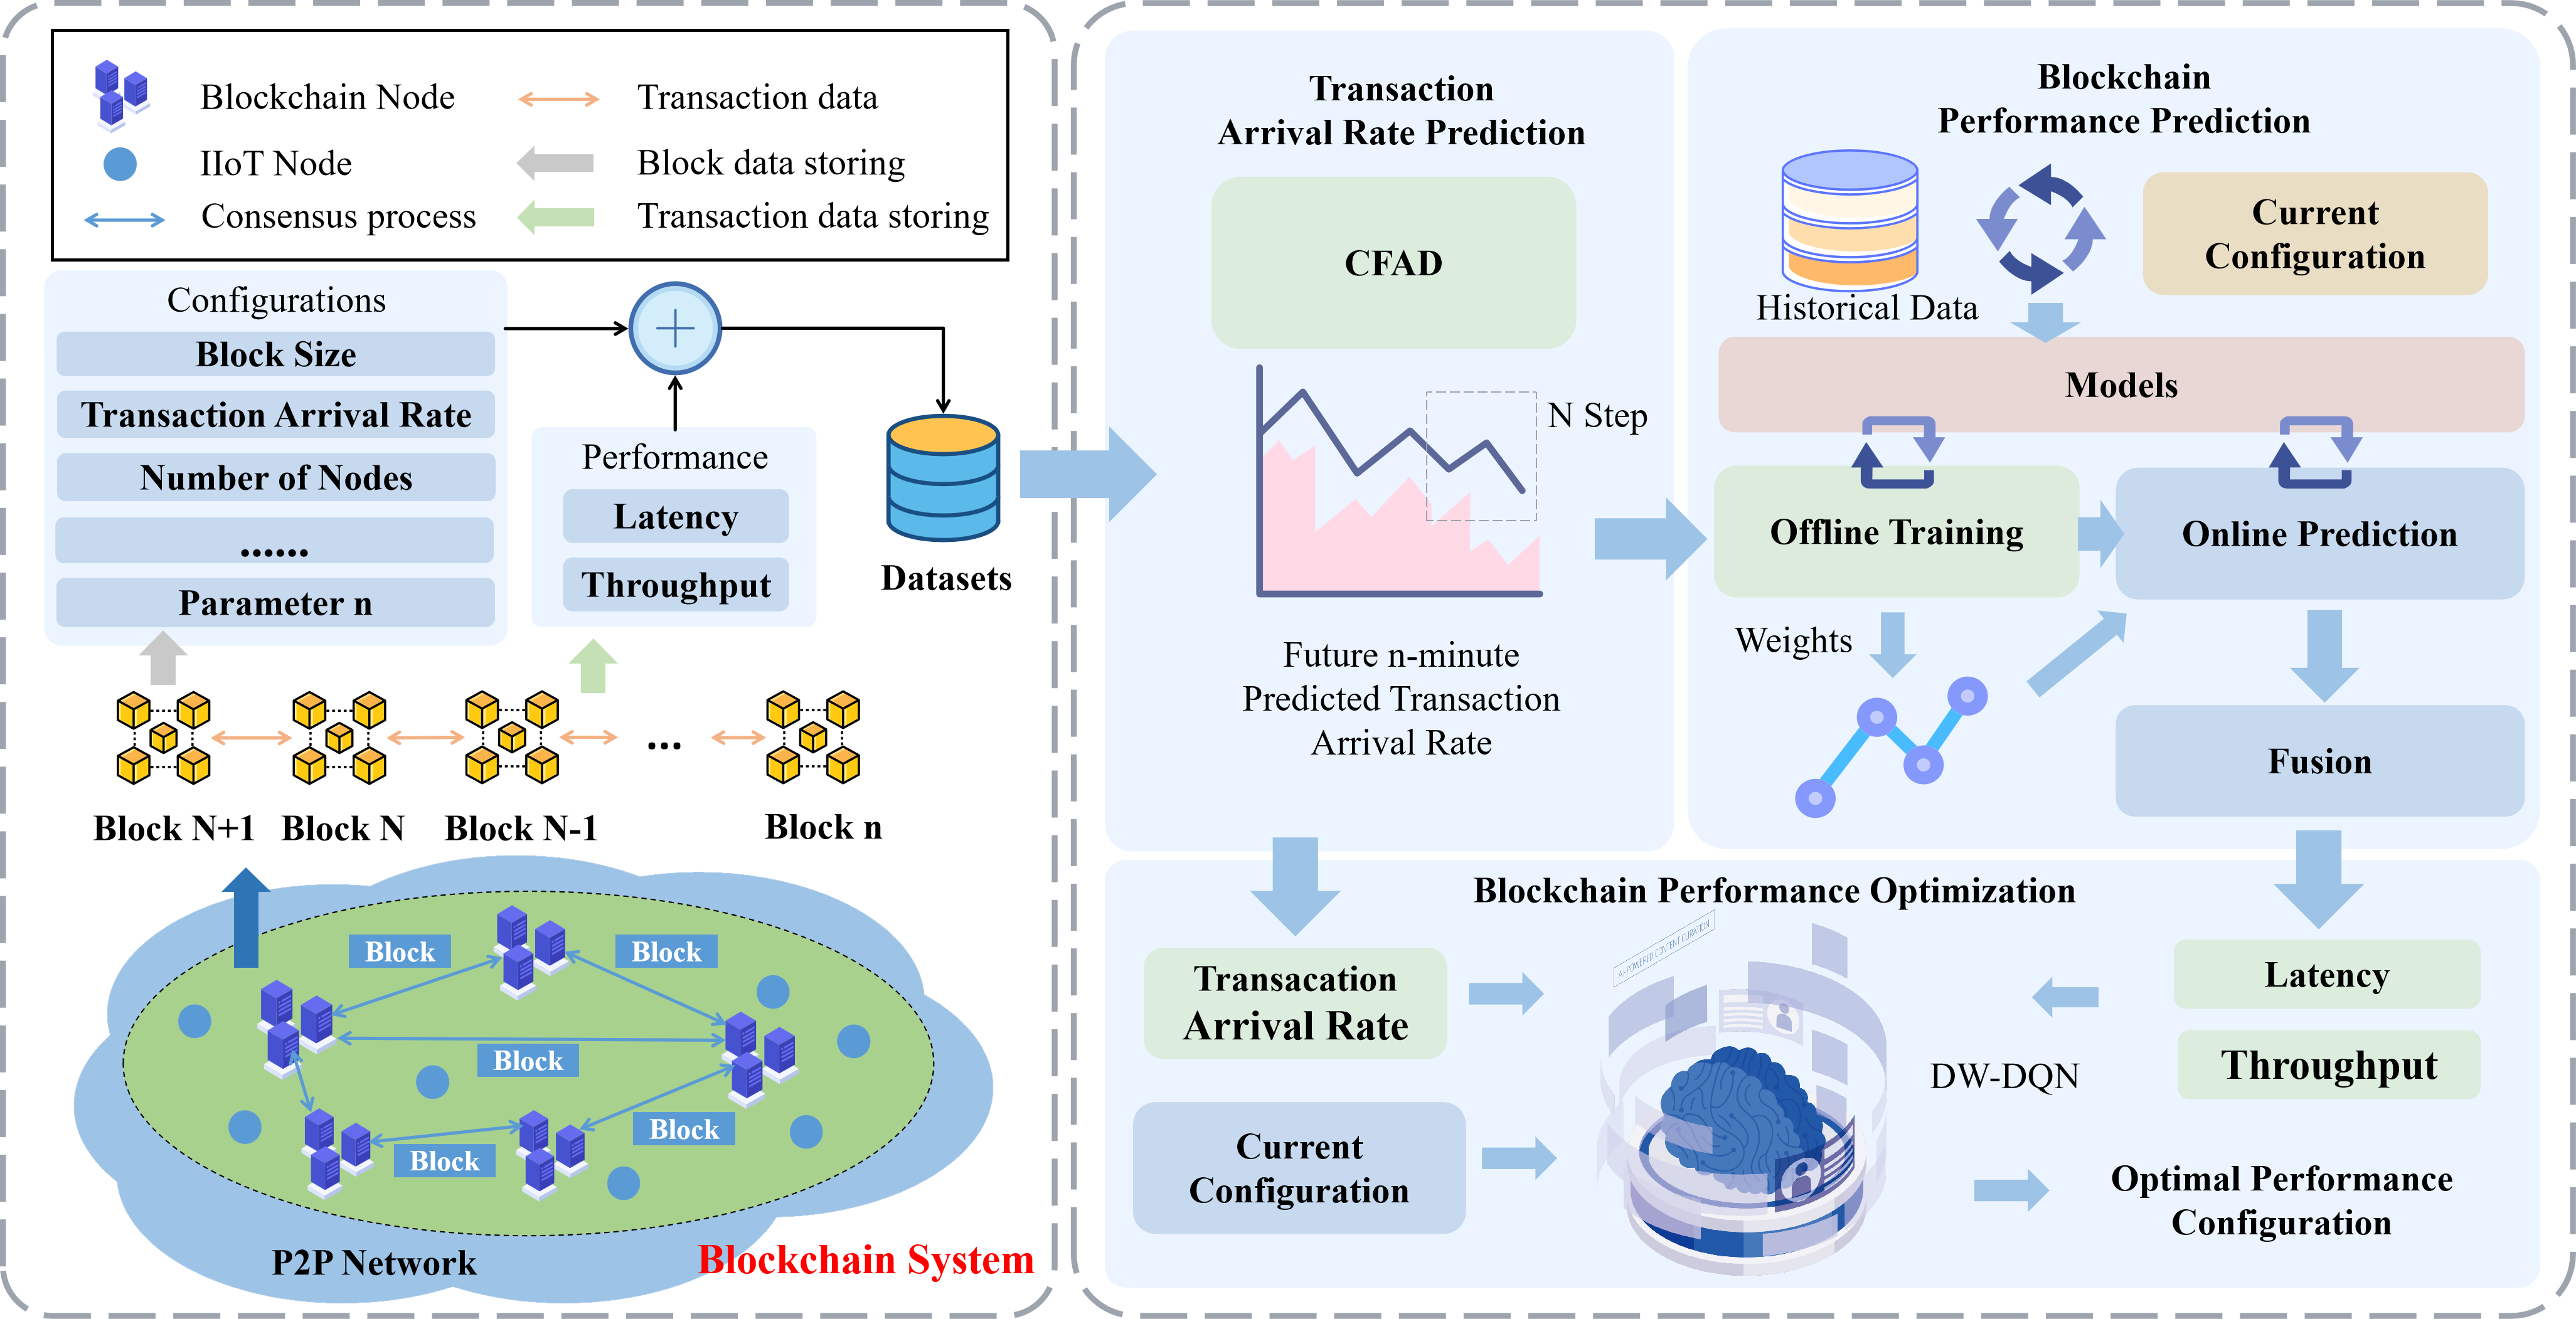
\includegraphics[width=\textwidth]{figures/overallframe.png}
	\caption{The framework of ChainOptNet.}
	\label{fig:overallframe}
\end{figure*}

\noindent
\textbf{(1) Transaction arrival rate prediction:}
The Convolutional Feature Aggregation and Distribution (CFAD) model predicts future transaction arrival rates from historical transaction data by effectively capturing temporal dependencies and local fluctuation patterns.



\noindent
\textbf{(2) Blockchain performance prediction:}
A multi-model collaborative prediction framework integrates seven machine learning models, including Linear Regression, Bayesian Ridge Regression, Decision Tree Regressor, Support Vector Regression, Gradient Boosting Regressor, Random Forest Regressor, and eXtreme Gradient Boosting Regressor, to estimate blockchain performance metrics such as latency and throughput. The prediction results are further fused using an inverse error-weighted ensemble strategy, thereby improving prediction robustness and accuracy.



\noindent
\textbf{(3) Blockchain performance optimization:}
A Dynamic Weight Deep Q-Network (DW-DQN) dynamically determines the optimal block size. Specifically, the optimization module consists of a DQN-based block-size controller and a trend-aware reward weighting module. The DQN learns the optimal block-size adjustment policy, while the reward weighting module adaptively computes the relative importance of latency and throughput according to recent performance trends, enabling adaptive multi-objective optimization.

%\begin{figure*}[thbp] \centering
%	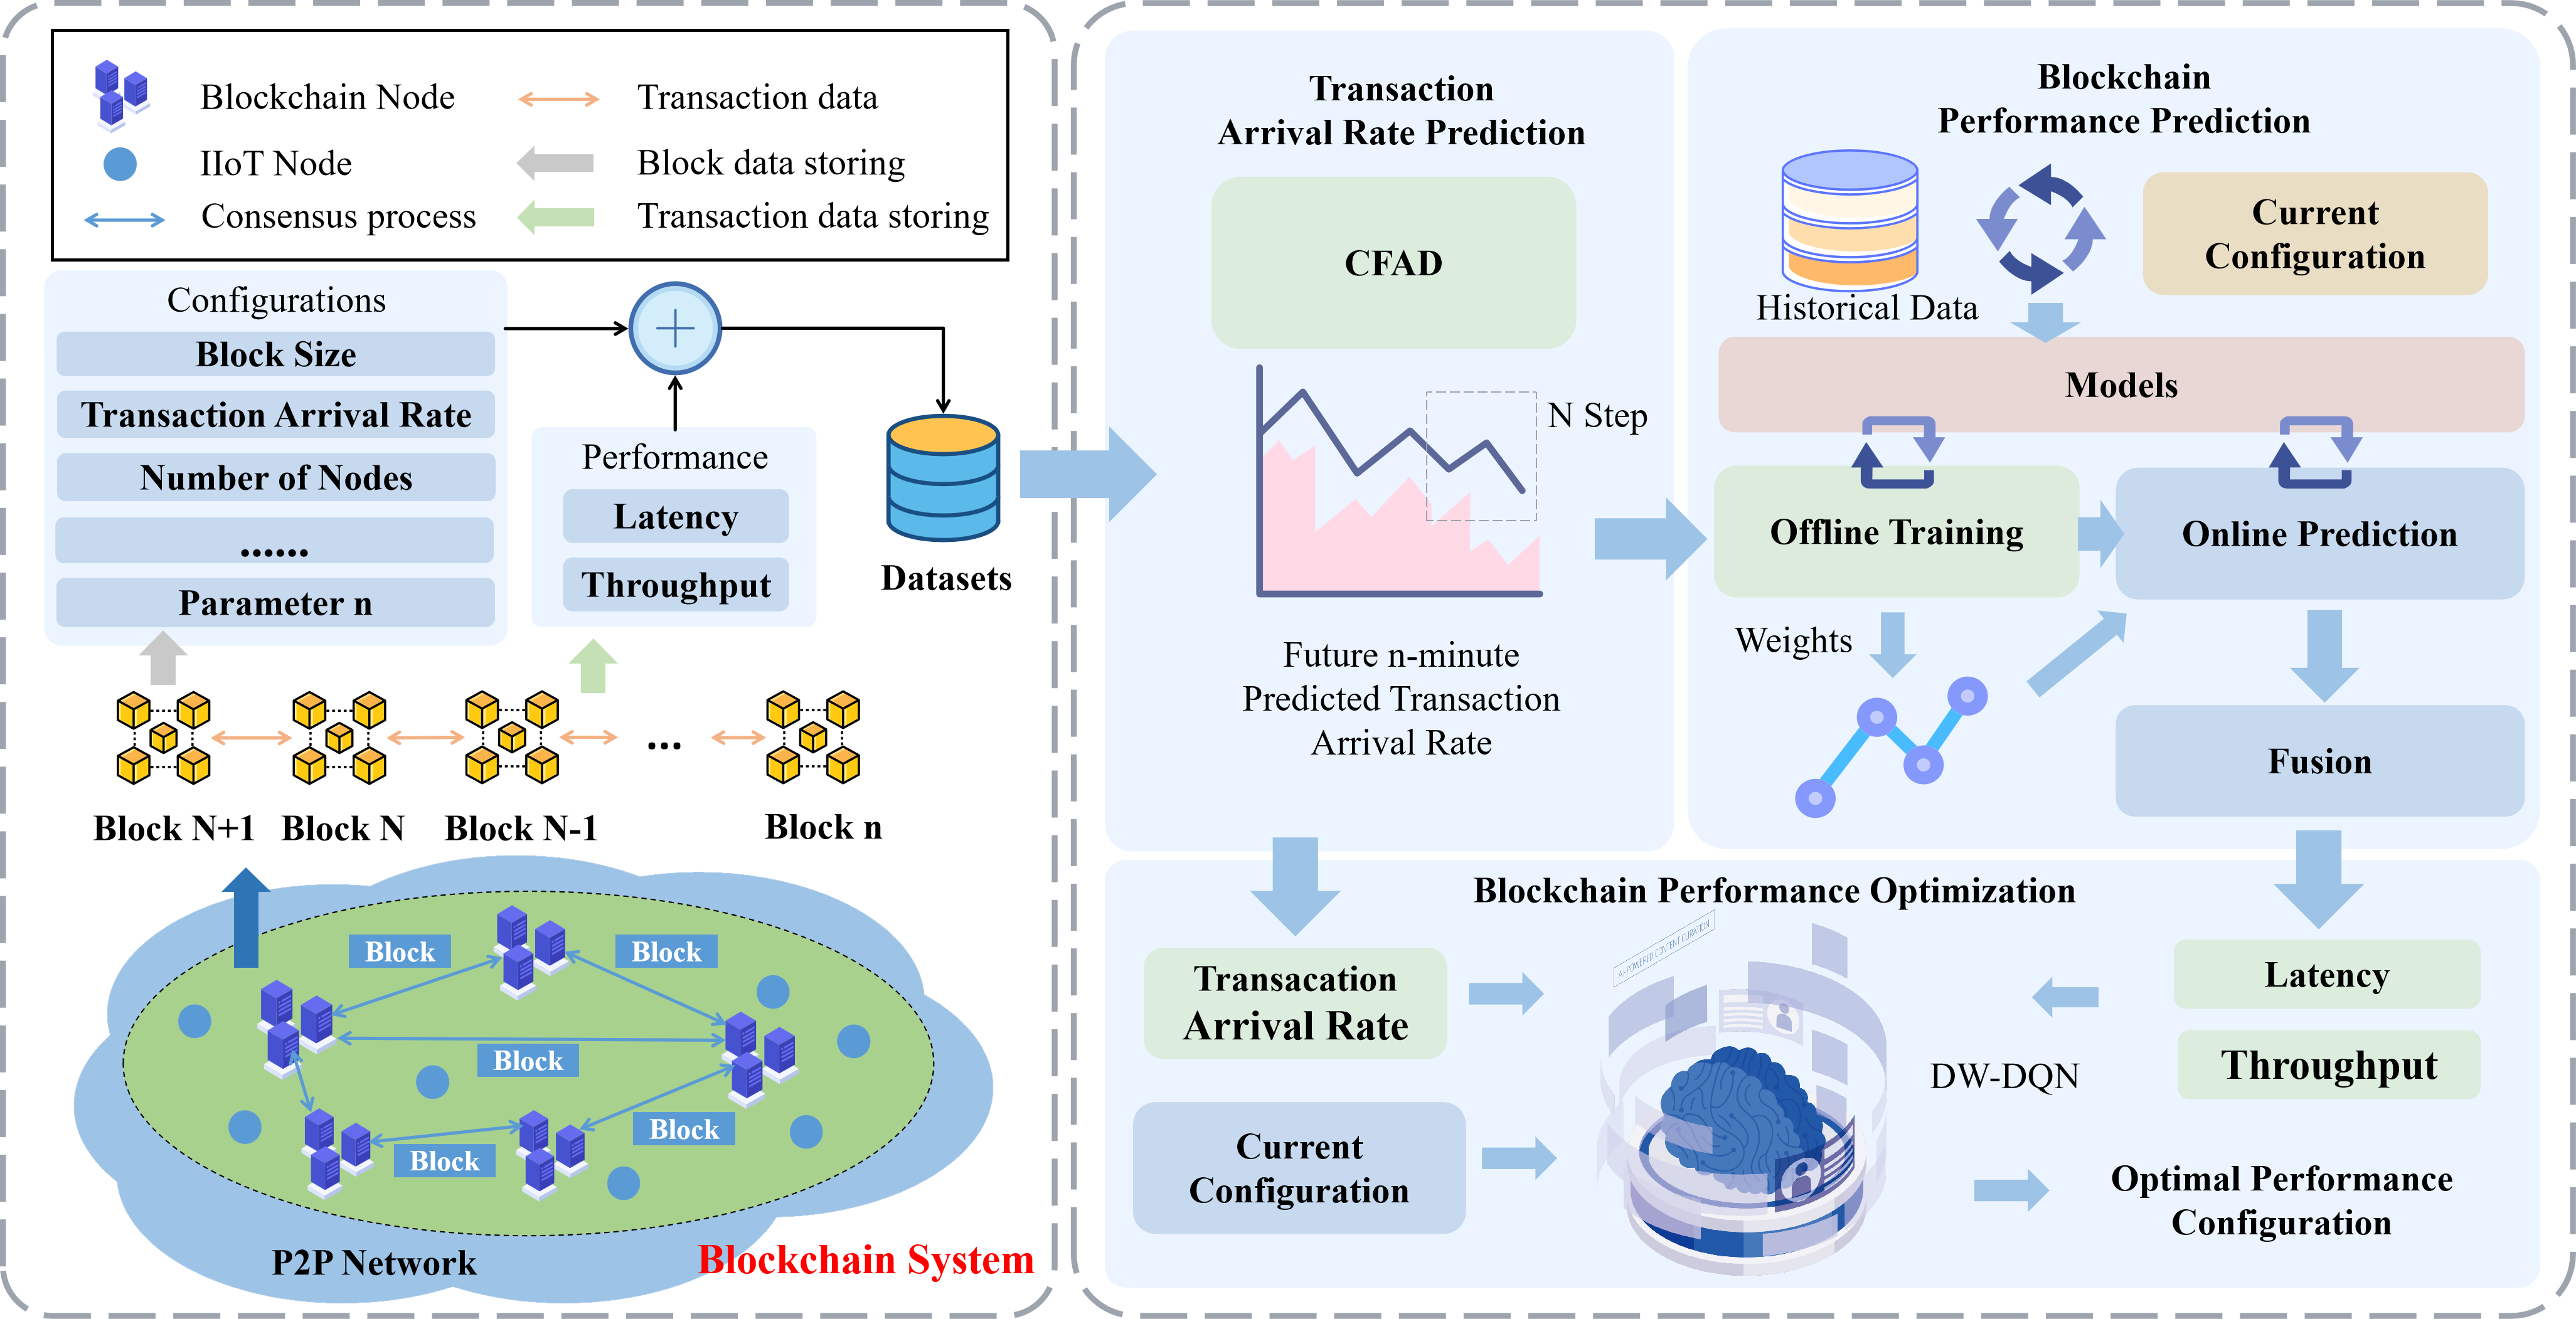
\includegraphics[width=0.8\textwidth]{figures/overallframe.png}
%	\caption{The framework of ChainOptNet.} \label{fig:overallframe}
%\end{figure*}


\subsection{Prediction of transaction arrival rate}
\vspace{6pt}
Inspired by the recently proposed SOFTS model \citep{han2024softs}, which demonstrates efficient and scalable performance in multivariate time series forecasting via its centralized STAR (STar Aggregate-Redistribute) module, we create a modified version specifically for predicting blockchain transaction arrival rates. Unlike SOFTS, which focuses on general multivariate forecasting across a variety of domains, our approach adapts and simplifies the centralized interaction mechanism by incorporating convolutional operations for both temporal and channel-wise modeling, making it better suited to the characteristics of blockchain transaction data. This leads to the creation of the Convolutional Feature Aggregation and Distribution (CFAD) framework, which preserves SOFTS' low complexity advantage while improving its suitability for blockchain-specific scenarios.

To address the challenges of blockchain performance optimization, particularly in accurately predicting transaction arrival rates, we propose the Convolutional Feature Aggregation and Distribution (CFAD) framework. This framework is intended to forecast multivariate transaction arrival rates efficiently, with less computational complexity than traditional methods. 
%The key innovation of CFAD is its use of Convolutional Neural Networks (CNNs) for feature aggregation and distribution, rather than traditional pooling or MLP approaches.
This method allows the model to capture both spatial and temporal dependencies in blockchain transaction data, which improves prediction accuracy and system performance. As shown in Figure~\ref{fig:timeseries}, the CFAD framework consists of three main components: sequence embedding, the Convolutional Feature Aggregation and Distribution Module (CFADM), and convolutional output projection.

\subsubsection{Sequence embedding}
\vspace{6pt}
The sequence embedding component of CFAD treats the entire transaction time series as a single "patch" processed through a 1D convolutional layer. This approach avoids the dimensionality expansion typically caused by patch embedding methods and preserves the temporal relationships in the data. By using a convolutional layer with a kernel size of 1 and 'same' padding, CFAD efficiently preserves the temporal relationships without dimensionality expansion:
\begin{equation}
	S_0 = \text{Conv1D}_{\text{kernel=1}}(X), \quad X \in \mathbb{R}^{L \times C}
\end{equation}
where $X$ represents the input transaction data with $L$ time steps and $C$ features (channels).

\begin{figure*}[htbp]
	\centering
	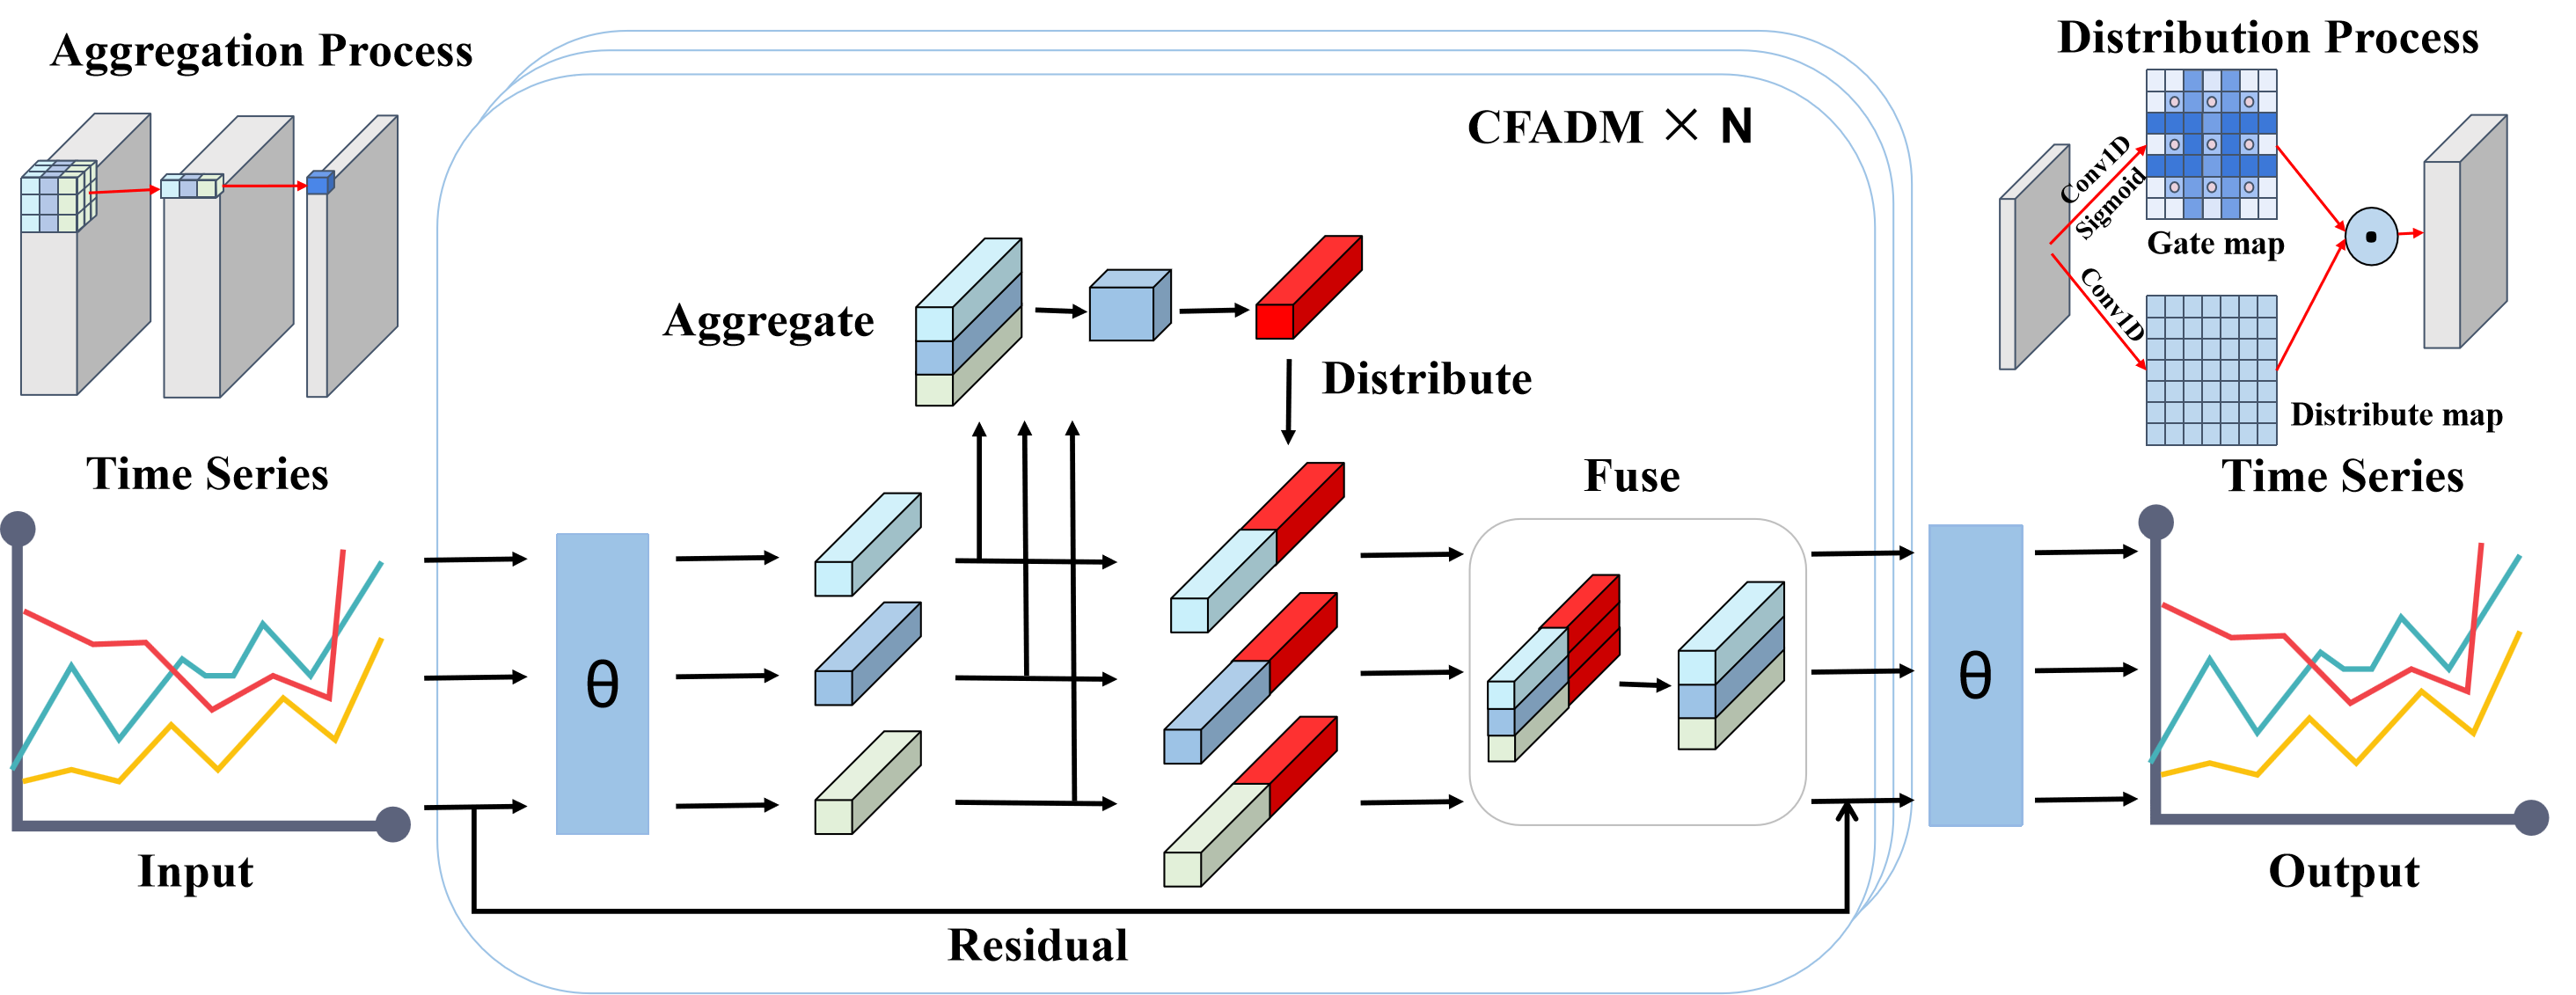
\includegraphics[width=1\textwidth]{figures/timeseries.png}
	\caption{The framework of CFAD.} \label{fig:timeseries}
\end{figure*}

\subsubsection{Convolutional feature aggregation and distribution module (CFADM)}
\vspace{6pt}
The Convolutional Feature Aggregation and Distribution Module (CFADM) is CFAD's core component, which aggregates and distributes features from blockchain transaction data. Formally,
\begin{equation}
	S_N = \text{CFADM}(S_0)
\end{equation}
where $S_N$ denotes the output of the $N$-th CFADM layer. The module has two phases:

\textbf{Aggregation Phase}:
During this phase, dual-layer $3\times3$ convolutions with 'same' padding and ReLU activation are used to aggregate temporal features from the input sequence. The aggregation process enables the model to learn implicit temporal dependencies throughout the sequence, resulting in a rich global feature representation of the transaction data:
\begin{equation}
	S_i^{agg} = \text{Conv1D}_{\text{aggregate, kernel=3}}(S_{i-1})
\end{equation}
\begin{equation}
	S_i^{agg} = \text{ReLU}(S_i^{agg}), \quad i=1,2,\dots,N
\end{equation}
%\begin{align}
	%S_i^{agg} &= \text{Conv1D}_{\text{aggregate, kernel=3}}(S_{i-1}) \\ 
	%S_i^{agg} &= \text{ReLU}(S_i^{agg}), \quad i=1,2,\dots,N
%\end{align}
where $S_i^{agg}$ represents the aggregated feature at the $i$-th layer.

\textbf{Distribution Phase}:
To enhance the preservation of layer-wise input information, we concatenate the aggregated features with the pre-aggregation input $S_{i-1}$ before distribution, forming a richer feature representation for subsequent gating and distribution. Specifically, features are first concatenated along the channel dimension:
\begin{align}
	S_i^{concat} &= \text{Concat}(S_i^{agg}, S_{i-1})
\end{align}
where $\text{Concat}(\cdot)$ denotes concatenation along the channel dimension, allowing the model to integrate both pre-aggregation input features and aggregated features.

The concatenated features are then redistributed across channels using two $1\times1$ convolutional branches combined with a gating mechanism. The gating is implemented via a sigmoid activation to control the flow of information, allowing the model to dynamically adjust the importance of each feature:
%\begin{align}
%	G_i &= \sigma(\text{Conv1D}{\text{gate}}(S_i^{concat})) \\
%	D_i &= \text{Conv1D}{\text{distribute, kernel=1}}(S_i^{concat}) \\
%	S_i^{out} &= G_i \odot D_i
%\end{align}
\begin{equation}
	G_i = \sigma(\text{Conv1D}_{\text{gate}}(S_i^{concat}))
\end{equation}
\begin{equation}
	D_i = \text{Conv1D}_{\text{distribute, kernel=1}}(S_i^{concat})
\end{equation}
\begin{equation}
	S_i^{out} = G_i \odot D_i
\end{equation}
where $\sigma(\cdot)$ denotes the sigmoid activation function for gating, and $\odot$ denotes element-wise multiplication. This step ensures that the most relevant features, enriched by both the current layer input and the aggregated global context, are distributed to subsequent layers for accurate prediction.

\subsubsection{Convolutional output projection}
\vspace{6pt}
Let $S_N$ represent the output of the $N$-th CFADM layer, which encodes aggregated and distributed temporal features. After the CFADM layers, the final feature representation is passed through a $1\times1$ convolutional layer to project the aggregated and distributed features into the predicted transaction arrival rates. Compared to a traditional fully connected layer, this convolutional output layer preserves the sequence's temporal structure and allows for localized prediction, which is especially useful for multi-step predicting:
\begin{equation}
	Y = \text{Conv1D}_{\text{out, kernel=1}}(S_N)
\end{equation}
where $Y \in \mathbb{R}^{L' \times 1}$ represents the predicted transaction arrival rates for future $L'$ time steps.



\subsection{Blockchain performance prediction model}
\vspace{6pt}

To address the limitations of single machine learning models in capturing complex interactions among features, this study proposes a multi-model collaborative prediction framework that combines seven different machine learning algorithms. This framework enhances predictive accuracy and adaptability in volatile blockchain environments by leveraging model diversity and dynamic weighting.

The proposed framework integrates the following base regressors: Linear Regression (LR), Bayesian Ridge Regression (BYR), Decision Tree Regressor (DTR), Bagging Regressor (BR), Gradient Boosting Regressor (GBR), Random Forest Regressor (RFR), and eXtreme Gradient Boosting (XGB). These models cover both parametric and non-parametric domains, allowing the ensemble to capture a wide range of data characteristics, including linear dependencies and complex nonlinear patterns.

Figure~\ref{fig:multimodelframework} depicts the complete workflow for the proposed multi-model framework. It is divided into two major stages: (i) an offline training phase, in which base learners are trained on enriched features and weighted using inverse-error-based softmax; and (ii) an online prediction phase, in which model weights are dynamically updated using a sliding window of recent observations to maintain adaptability under changing conditions.


Let the input feature vector be denoted as \(X = [x_1, x_2, \cdots, x_n] \in \mathbb{R}^d\), comprising normalized system parameters such as transaction arrival rate, block size, and number of ordering nodes. The corresponding target vector \(Y \in \mathbb{R}^k\) represents performance indicators including latency and throughput.

Prior to model training, the input features are standardized using z-score normalization:
\begin{equation}
	X_{\text{scaled}} = \frac{X - \mu}{\sigma},
\end{equation}
where \(\mu\) and \(\sigma\) denote the mean and standard deviation of each feature, respectively.

To enrich the feature representation, second-order interactions are explicitly computed as follows:
\begin{equation}
	X_{\text{interaction}} = [X \otimes X],
\end{equation}
where \(\otimes\) denotes the outer product of the feature vector. The resulting interaction terms are concatenated with the normalized input to form an extended feature vector:
\begin{equation}
	X_{\text{extended}} = [X_{\text{scaled}}, X_{\text{interaction}}].
\end{equation}

Each base model \(f_m(\cdot)\), parameterized by \(\theta_m\), produces an individual prediction \(\hat{Y}_m\) as follows:
\begin{equation}
	\hat{Y}_m = f_m(X_{\text{extended}}; \theta_m).
\end{equation}

To evaluate model performance, the Mean Absolute Error (MAE) is adopted. Let the total number of samples be \(N\), and assume each sample’s true label is \(Y_i \in \mathbb{R}^k\), the MAE of model \(m\) over the dataset is computed as follows:
\begin{equation}
	\text{MAE}_m = \frac{1}{N} \sum_{i=1}^{N} \left\| \hat{Y}_{i,m} - Y_i \right\|_1,
\end{equation}
where \(\|\cdot\|_1\) denotes the element-wise \(L_1\)-norm across the performance metrics.

Based on these MAE scores, an inverse-error-based softmax function determines the ensemble weights:
\begin{equation}
	W_m = \frac{\exp(-\text{MAE}_m / T)}{\sum_{j=1}^{M} \exp(-\text{MAE}_j / T)},
\end{equation}
where \(T\) is a temperature hyperparameter controlling the sharpness of the distribution.

In the online prediction phase, model performance is continuously reassessed using a sliding window of the most recent \(N\) samples. At time step \(t\), let the windowed data be \(\{(X_{t-i}, Y_{t-i})\}_{i=0}^{N-1}\). The updated prediction error for model \(m\) is calculated as follows:
\begin{equation}
	\text{MAE}_m^{(t)} = \frac{1}{N} \sum_{i=0}^{N-1} \left\| f_m(X_{t-i}; \theta_m) - Y_{t-i} \right\|_1.
\end{equation}

The corresponding dynamic weight is:
\begin{equation}
	W_m^{(t)} = \frac{\exp(-\text{MAE}_m^{(t)} / T)}{\sum_{j=1}^{M} \exp(-\text{MAE}_j^{(t)} / T)}.
\end{equation}
and the ensemble prediction becomes:
\begin{equation}
	\hat{Y}^{(t)} = \sum_{m=1}^{M} W_m^{(t)} \cdot \hat{Y}_m^{(t)}.
\end{equation}

While \(\hat{Y}^{(t)}\) serves as the final output of the ensemble during the inference phase, the training process aims to optimize the base model parameters \(\{\theta_m\}_{m=1}^{M}\) by minimizing a composite loss function that  reflects the accuracy of both latency and throughput predictions.

To ensure balanced learning across both objectives, the training process minimizes the following composite loss function:
\begin{equation}
	L = \alpha L_{\text{latency}} + (1 - \alpha) L_{\text{throughput}},
\end{equation}
where \(\alpha \in [0,1]\) is a hyperparameter controlling the relative importance of latency and throughput prediction. Cross-validation using grid search determines the optimal \(\alpha\) value.

\begin{figure}
	\centering
	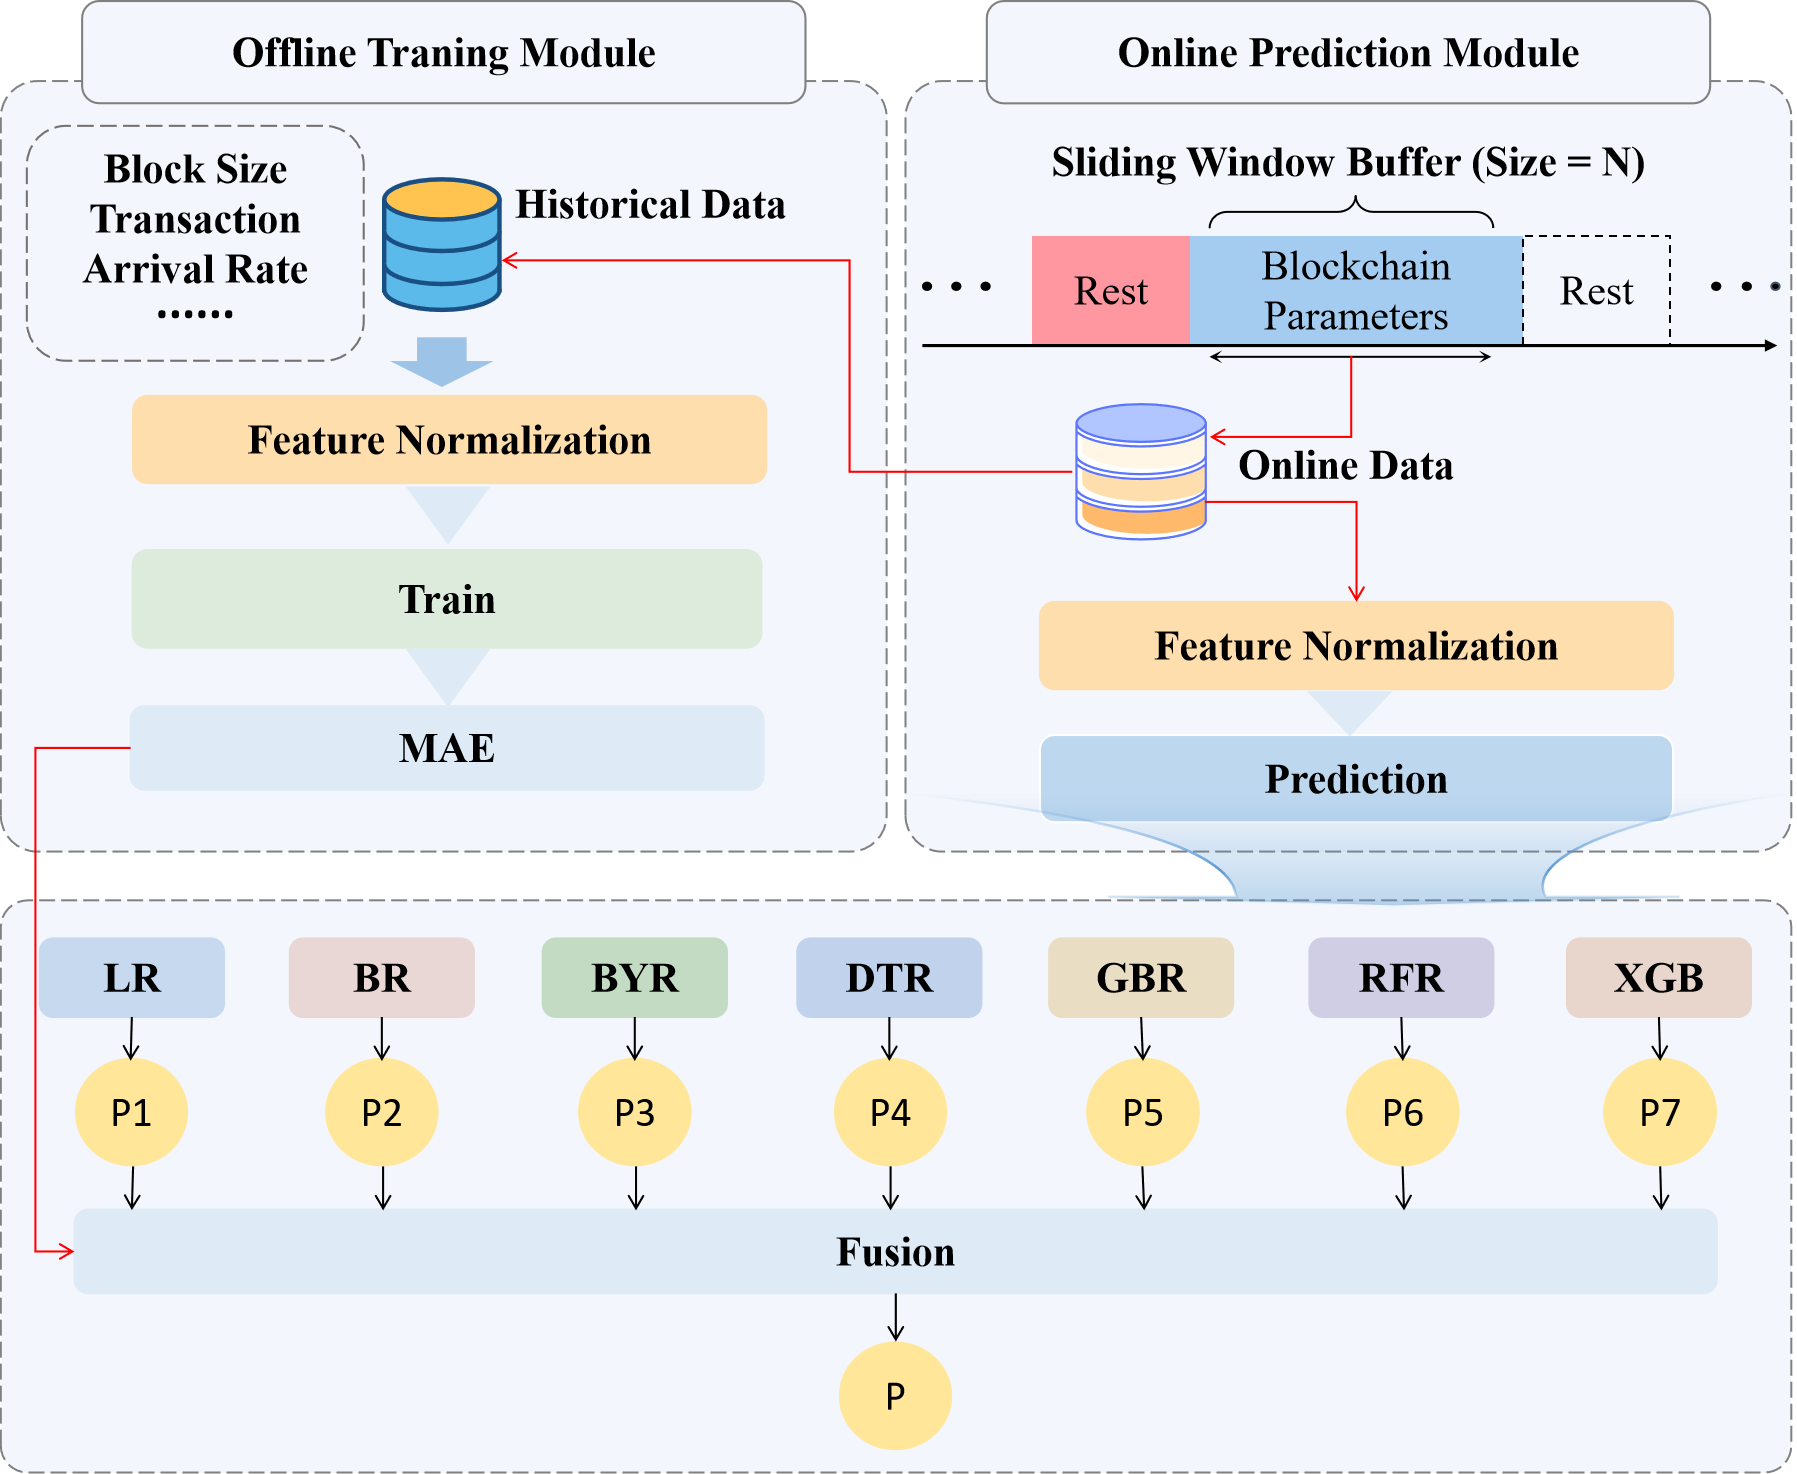
\includegraphics[width=.9\columnwidth]{figures/multimodelframework.png}
	\caption{The framework of multi-model performance prediction.}
	\label{fig:multimodelframework}
\end{figure}



\subsection{Blockchain performance optimization with DW-DQN}
\vspace{6pt}
The proposed Dynamic Weight Deep Q-Network (DW-DQN) framework is intended to address the limitations of traditional reinforcement learning approaches in multi-objective optimization tasks within blockchain environments, particularly in the dynamic adjustment of block size to optimize throughput and latency. Unlike traditional Deep Q-Networks (DQNs), which use a static reward formulation, DW-DQN combines a DQN-based block-size controller with a trend-aware dynamic reward weighting module. The DQN learns the action policy, while the weighting module deterministically updates the latency and throughput weights according to recent system performance trends.

\begin{figure}
	\centering
	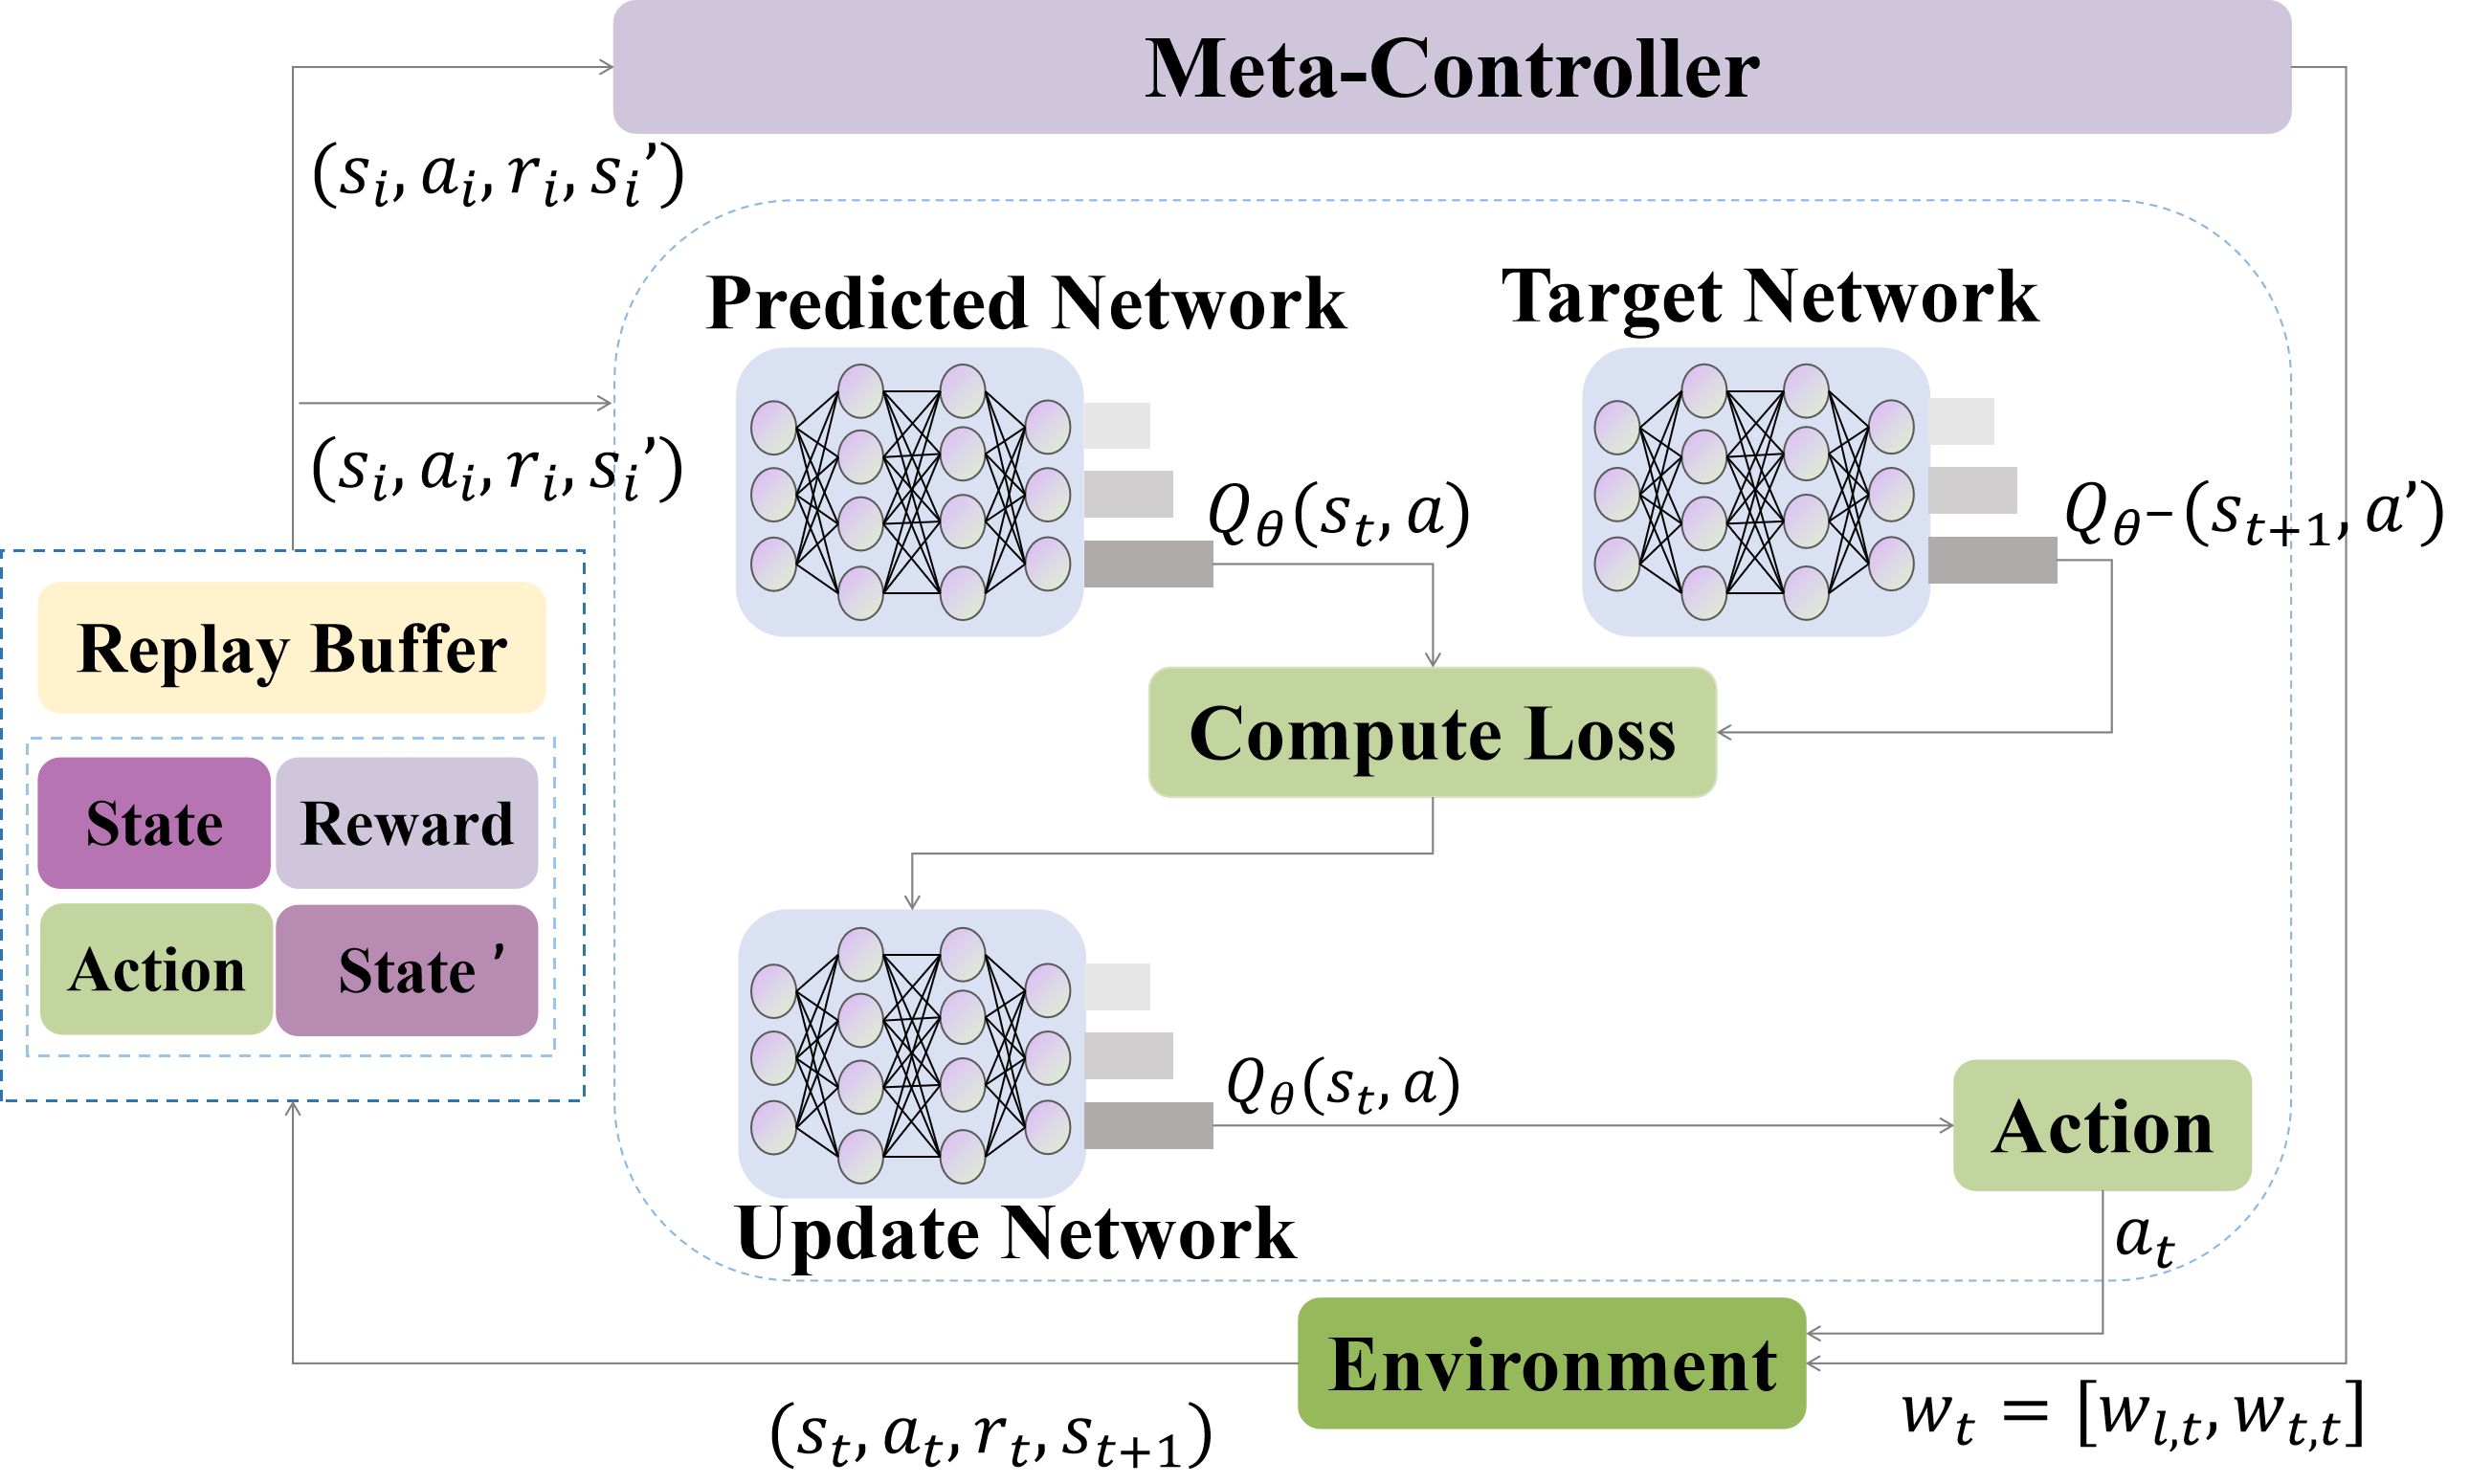
\includegraphics[width=.9\columnwidth]{figures/dwdqnmodel.png}
	\caption{The framework of DW-DQN.}
	\label{fig:dwdqnmodel}
\end{figure}

%To put this design into practice, the entire training procedure, including dynamic weight computation, Q-network optimization, and performance evaluation, is described in Algorithm~\ref{alg:dwdqn}.

Figure~\ref{fig:dwdqnmodel} depicts the architecture and interconnections of the system's components, providing a comprehensive overview of the proposed DW-DQN framework. The framework is made up of two coordinated components: (1) a DQN agent that learns an optimal block-size adjustment policy from environmental interactions, and (2) a trend-aware reward weighting module that computes the weight vector used in reward computation. The state information is used by the DQN for action selection and by the weighting module for reward prioritization.



Formally, the learning process is modeled as a Markov Decision Process (MDP) $(\mathcal{S}, \mathcal{A}, \mathcal{P}, \mathcal{R}, \gamma)$, where $\mathcal{S}$ denotes the state space, $\mathcal{A}$ represents the action space, $\mathcal{P}$ denotes the state transition probabilities, $\mathcal{R}$ represents the reward function, and $\gamma \in [0,1)$ denotes the discount factor. At time step $t$, the system state is represented as follows:
\begin{equation}
	s_t = [\lambda_t, b_t, n_t, l_t, \tau_t]
\end{equation}
where $\lambda_t$ denotes the transaction arrival rate, $b_t$ represents the current block size, $n_t$ denotes the number of ordering nodes, $l_t$ represents the average latency, and $\tau_t$ denotes the average throughput. The action $a_t$ corresponds to a discrete change in block size $a_t \in \{-\Delta b, 0, +\Delta b\}$, where $\Delta b$ is the step size.

Instead of a fixed scalar reward, the DW-DQN framework utilizes a dynamically weighted reward function defined as follows:
\begin{equation}
	r_t = \omega_{l,t} r_t^{(l)} + \omega_{\tau,t} r_t^{(\tau)}
\end{equation}
\begin{equation}
	r_t^{(l)} = -|l_t - l^*|
\end{equation}
\begin{equation}
	r_t^{(\tau)} = \tau_t / \tau^*
\end{equation}
where $r_t^{(l)}$ penalizes latency deviation from a target latency $l^*$, and $r_t^{(\tau)}$ reflects normalized throughput performance against a target $\tau^*$. The weights $\omega_{l,t}$ and $\omega_{\tau,t}$ are dynamically computed at each time step by the trend-aware weighting module, subject to the constraint $\omega_{l,t} + \omega_{\tau,t} = 1$. These weights are not predicted by an additional neural network. Instead, they are derived from recent latency and throughput trends so that the reward function can emphasize the objective that is currently changing more sharply.

The DQN agent approximates the action-value function $Q_\theta(s_t, a_t)$, using a neural network with parameters $\theta$. The network is trained to minimize the temporal-difference loss:
\begin{equation}
	L(\theta)=\mathbb{E}_{\mathcal{D}}\left[\left(r+\gamma\max_{a'}Q_{\theta^-}(s',a')-Q_\theta(s,a)\right)^2\right]
\end{equation}
where $\theta^-$ are the parameters of the target network $Q_{\theta^-}$, which are periodically updated from $\theta$, and $\mathcal{D}$ denotes the replay buffer that stores transitions $(s_t, a_t, r_t, s_{t+1})$.

The trend-aware weighting module maintains recent latency and throughput observations and computes their trends via first-order differences. A normalized ratio is then used to determine the relative importance of latency and throughput.
\begin{equation}
	\text{latency\_importance} = \frac{|\text{trend}_l|}{|\text{trend}_l| + |\text{trend}_\tau| + \varepsilon}
\end{equation}
\begin{equation}
	 \text{throughput\_importance} = 1 - \text{latency\_importance}
\end{equation}
where \(\text{trend}_l\) and \(\text{trend}_\tau\) denote the mean first-order differences of recent latency and throughput, respectively, and \(\varepsilon\) is a small constant to avoid division by zero. These importance scores are passed through a softmax layer to ensure probabilistic normalization. The resulting weights \(\omega_{l,t} \text{ and } \omega_{\tau,t}\) are then clipped to lie within a specified range \([\omega_{\min}, \omega_{\max}]\), and re-normalized to enforce \(\omega_{l,t} + \omega_{\tau,t} = 1\).

The objective of the DQN agent is to maximize the expected cumulative dynamically weighted reward:
\begin{equation}
	R_t = \sum_{k=0}^\infty \gamma^k r_{t+k}
\end{equation}
where \(R_t\) denotes the cumulative discounted reward starting at time step \(t\), based on the dynamically weighted reward formulation. Only the Q-network parameters are learned through temporal-difference updates; the reward weights are computed by the deterministic trend-aware module and are not updated by a separate learned policy.

This design allows the action policy to be learned by DQN while the reward priorities are adapted online according to observed network behavior. The DW-DQN framework demonstrates robust adaptability by dynamically modulating reward priorities through a deterministic trend-aware rule, significantly improving blockchain system performance under a variety of operational scenarios.

%\begin{algorithm}[htb]
%	\caption{DW-DQN Training Process}
%	\label{alg:dwdqn}
%	\begin{algorithmic}[1]
%		\Require 
%		Environment state space $\mathcal{S}$,\\ 
%		Action space $\mathcal{A}$,\\
%		Reward function $r(s, a, w_L, w_T)$,\\
%		Weighting update interval $T_w$,\\
%		Dynamic weighting function $\phi(\delta)$,\\
%		Initial Q-network parameters $\theta$,\\
%		Target network parameters $\theta^-$,\\
%		Replay buffer $\mathcal{D}$,\\
%		Learning rate $\alpha$,\\
%		Discount factor $\gamma$,\\
%		Batch size $B$
		
%		\Ensure 
%		Trained Q-network parameters $\theta^*$ and optimal blockchain configuration BPC
		
%		\State Initialize Q-network $Q_\theta(s, a)$ and target network $Q_{\theta^-}(s, a)$
%		\State Initialize dynamic weights: $w_L \gets w_0$, $w_T \gets w_0$
%		\State Initialize replay buffer $\mathcal{D} \gets \emptyset$
%		\State Initialize best performance metric $\mathcal{P}_{\text{best}} \gets -\infty$
%		\State Initialize best configuration BPC $\gets \emptyset$
		
%		\For{episode $=1,2,\dots$}
%		\State Reset environment; observe initial state $s_0$
%		\For{step $t=1,2,\dots$}
%		\State Select action $a_t$ using $\epsilon$-greedy policy w.r.t. $Q_\theta(s_t, a)$
%		\State Execute $a_t$; observe reward $r_t$, next state $s_{t+1}$, latency deviation $\delta_L$, throughput deviation $\delta_T$
%		\State Store transition $(s_t, a_t, r_t, s_{t+1})$ in $\mathcal{D}$
		
%		\If{$t \bmod T_m = 0$} {Meta-controller update}
%		\State Update latency weight: $w_L \gets \phi(\delta_L)$
%		\State Update throughput weight: $w_T \gets \phi(\delta_T)$
%		\EndIf
		
%		\State Sample mini-batch of $B$ transitions $(s_j, a_j, r_j, s'_j)$ from $\mathcal{D}$
%		\State Compute targets: $y_j \gets r_j + \gamma \cdot \max_{a'} Q_{\theta^-}(s'_j, a')$
%		\State Compute loss: $\mathcal{L} \gets \frac{1}{B}\sum_j (Q_\theta(s_j,a_j) - y_j)^2$
%		\State Update Q-network: $\theta \gets \theta - \alpha \nabla_\theta \mathcal{L}$
		
%		\State Every $C$ steps update target network: $\theta^- \gets \theta$
		
%		\State Evaluate performance metric $\mathcal{P}_t$ under $a_t$
%		\If{$\mathcal{P}_t > \mathcal{P}_{\text{best}}$}
%		\State $\mathcal{P}_{\text{best}} \gets \mathcal{P}_t$
%		\State BPC $\gets$ configuration corresponding to $a_t$
%		\EndIf
%		\EndFor
%		\EndFor
		
%		\State \Return $\theta^* \gets \theta$, Best Performance Configuration BPC
%		\State {Apply BPC to update blockchain system parameters}
%	\end{algorithmic}
%\end{algorithm}





\section{Experimental evaluation and analysis}\label{sec:experiments}

This section contains a series of experiments designed to assess the performance and effectiveness of the proposed methods. Qualitative comparisons with related work are also provided to highlight the novelty and benefits.

\subsection{Experimental settings}
\vspace{6pt}
\subsubsection{Experimental design}
\vspace{6pt}
We conducted three sets of experimentss:
(1) predicting transaction arrival rates, (2) predicting blockchain performance through inverse error ensemble learning, and (3) optimizing blockchain performance.

\subsubsection{Datasets}
\vspace{6pt}
In Experiment 1 used an open-source dataset of parking lot records collected in real-world scenarios to predict transaction arrival rates. Although originally designed for parking behavior analysis, the dataset's realistic temporal characteristics make it suitable for modeling blockchain transaction arrivals.

For Experiments 2 and 3, we used the HFBDP dataset, an open-source blockchain performance dataset compiled by \citep{wang2023learningchain} using Hyperledger Fabric. The dataset has five key parameters: orderer node count ({3, 5, 7, 9}), transaction arrival rate ({10, 15, 20, \ldots, 200}), block size ({10, 15, 20, \ldots, 800}), latency, and throughput. These parameters were applied to the blockchain performance prediction and optimization tasks, respectively.

\subsubsection{Comparable methods}
\vspace{6pt}
To comprehensively evaluate the effectiveness of the proposed ChainOptNet framework, representative baseline methods were selected for each task.

For transaction arrival rate prediction, we compared the proposed CFAD model with several representative time-series forecasting models, including Autoformer, Informer, Transformer, LSTM, GRU, LightTS, MLP, and a blockchain-oriented temporal prediction baseline \citep{wang2023learningchain}. These methods cover recurrent neural networks, Transformer-based architectures, lightweight forecasting models, and domain-specific prediction methods.

For blockchain performance prediction, the proposed multi-model collaborative prediction framework was compared with several widely used regression models, including Linear Regression (LR), Bayesian Ridge Regression (BR), Bayesian Regularization (BYR), Decision Tree Regression (DTR), Gradient Boosting Regression (GBR), Random Forest Regression (RFR), and eXtreme Gradient Boosting (XGB). These models represent linear regression, probabilistic regression, decision tree learning, and ensemble learning methods that are widely adopted for blockchain performance prediction.

For blockchain performance optimization, we compared the proposed DW-DQN with representative non-RL optimization settings, including fixed block-size configurations and a prediction-driven score-based adjustment strategy \citep{wang2023learningchain}. Such methods adjust parameters according to predefined performance scores or static configuration rules, whereas DW-DQN formulates block-size optimization as a reinforcement learning problem and dynamically adjusts reward weights according to network conditions, enabling more adaptive optimization under varying workloads.

To ensure fairness and reproducibility, all baseline methods were evaluated using identical datasets, preprocessing procedures, experimental settings, and evaluation metrics.

\subsubsection{Evaluation metrics}
\vspace{6pt}
To quantitatively evaluate the prediction and optimization performance of the proposed framework, three widely used regression metrics were adopted, namely Mean Absolute Error (MAE), Root Mean Square Error (RMSE), and Mean Absolute Percentage Error (MAPE). During model training, the Mean Squared Error (MSE) was employed as the optimization objective. These metrics provide a comprehensive evaluation of prediction accuracy, robustness, and generalization capability.

\textbf{Mean Squared Error (MSE):}
During model training, the Mean Squared Error (MSE) was used as the loss function to optimize model parameters. It is defined as

\begin{equation}
	\mathrm{MSE}=\frac{1}{N}\sum_{i=1}^{N}(y_i-\hat{y}_i)^2,
\end{equation}

where $N$ denotes the number of samples, $y_i$ is the ground-truth value, and $\hat{y}_i$ represents the corresponding prediction.

\textbf{Mean Absolute Error (MAE):}
MAE measures the average magnitude of prediction errors regardless of their direction and is formulated as

\begin{equation}
	\mathrm{MAE}=\frac{1}{N}\sum_{i=1}^{N}|y_i-\hat{y}_i|.
\end{equation}

A smaller MAE indicates higher prediction accuracy and better overall performance.

\textbf{Root Mean Square Error (RMSE):}
RMSE measures the standard deviation of prediction errors and places greater emphasis on larger errors. It is calculated as

\begin{equation}
	\mathrm{RMSE}=
	\sqrt{
		\frac{1}{N}
		\sum_{i=1}^{N}
		(y_i-\hat{y}_i)^2
	}.
\end{equation}

Lower RMSE values indicate better predictive performance and stronger robustness to large deviations.

\textbf{Mean Absolute Percentage Error (MAPE):}
MAPE evaluates prediction accuracy in terms of relative error and is defined as

\begin{equation}
	\mathrm{MAPE}
	=
	\frac{100\%}{N}
	\sum_{i=1}^{N}
	\left|
	\frac{y_i-\hat{y}_i}{y_i}
	\right|.
\end{equation}

MAPE is scale-independent and is particularly suitable for comparing prediction performance across different experimental settings.


\subsection{The performance of ChainOptNet}
\vspace{6pt}
\subsubsection{Prediction performance on transaction arrival rate}
\vspace{6pt}
To evaluate the generalization capability and robustness of the proposed Convolutional Feature Aggregation and Distribution (CFAD) model in predicting transaction arrival rates, experiments were conducted at three temporal granularities: 1-minute, 2-minute, and 5-minute intervals.


As shown in Figure~\ref{fig:time_forecast_results} and Table~\ref{tab:time_method_comparison}, CFAD achieves the lowest MAE and RMSE at all three evaluated time intervals and the lowest MAPE at the 2-minute and 5-minute intervals. At the 1-minute interval, Autoformer achieves a lower MAPE (0.2220) than CFAD (0.2486). CFAD's MAE and RMSE results are attributed to its global one-dimensional convolution-based sequence encoder, which preserves the inherent sequential structure of transaction data, allowing for better capture of fine-grained temporal dependencies and improved responsiveness to sudden fluctuations.

\begin{figure}
	\centering
	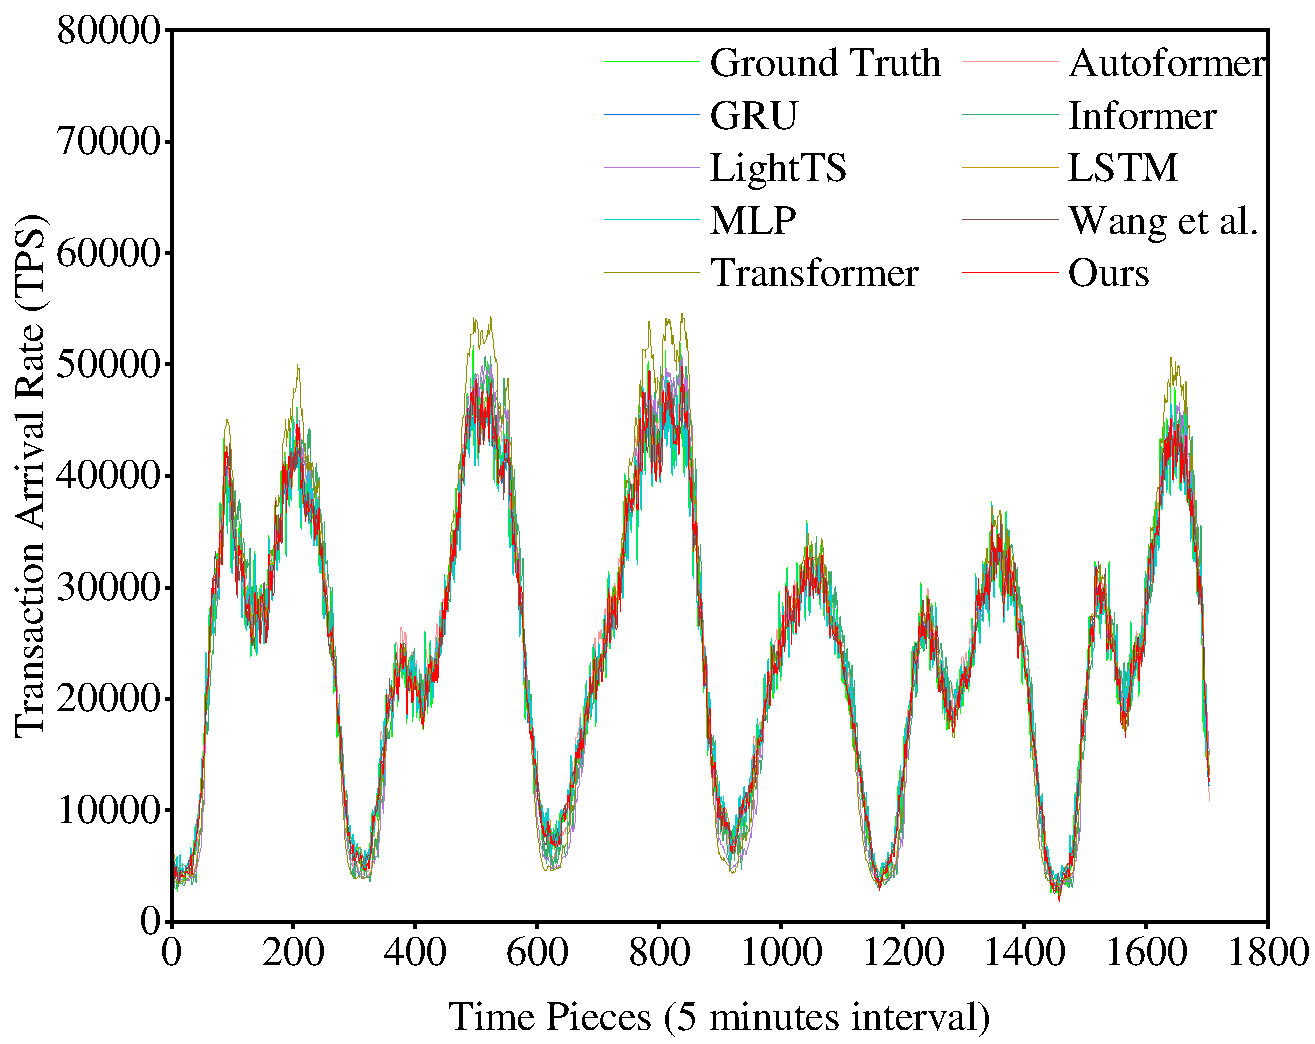
\includegraphics[width=.9\columnwidth]{figures/time_forecast_results.pdf}
	\caption{Prediction results of different models}
	\label{fig:time_forecast_results}
\end{figure}

\begin{table*}[t]
	\centering
	\caption{Prediction performance comparison across different time intervals.}
	\label{tab:time_method_comparison}
	\renewcommand{\arraystretch}{1.2}
	\begin{tabular}{ccccccccccc}
		\toprule
		\multirow{2}{*}{\centering \textbf{Time periods}} & \multirow{2}{*}{\centering \textbf{Metrics}} & \multicolumn{9}{c}{\textbf{Methods}} \\
		\cmidrule{3-11}
		& & \textbf{Informer} & \textbf{LSTM} & \textbf{Transformer} & \textbf{GRU} & \textbf{MLP} & \textbf{AutoFormer} & \textbf{LightTS} & \textbf{Wang et al.} & \textbf{Ours} \\
		\midrule
		\multirow{3}{*}{1 minute}
		& MAE  & 0.0534 & 0.0404 & 0.0441 & 0.0405 & 0.0511 & 0.0430 & 0.0406 & 0.0406 & \textbf{0.0400} \\
		& RMSE & 0.0658 & 0.0526 & 0.0583 & 0.0529 & 0.0662 & 0.0552 & 0.0528 & 0.0529 & \textbf{0.0523} \\
		& MAPE & 0.2807 & 0.2861 & 0.2727 & 0.2849 & 0.3099 &\textbf{0.2220} & 0.2928 & 0.2699 & 0.2486 \\
		\midrule
		\multirow{3}{*}{2 minutes}
		& MAE  & 0.0564 & 0.0347 & 0.0432 & 0.0343 & 0.0419 & 0.0421 & 0.0401 & 0.0351 & \textbf{0.0337} \\
		& RMSE & 0.0721 & 0.0455 & 0.0542 & 0.0449 & 0.0547 & 0.0540 & 0.0512 & 0.0461 & \textbf{0.0441} \\
		& MAPE & 0.2232 & 0.1296 & 0.1772 & 0.1377 & 0.1713 & 0.1643 & 0.1580 & 0.1341 & \textbf{0.1275} \\
		\midrule
		\multirow{3}{*}{5 minutes}
		& MAE  & 0.0406 & 0.0282 & 0.0458 & 0.0277 & 0.0311 & 0.0324 & 0.0376 & 0.0293 & \textbf{0.0247} \\
		& RMSE & 0.0510 & 0.0368 & 0.0601 & 0.0360 & 0.0404 & 0.0416 & 0.0479 & 0.0387 & \textbf{0.0325} \\
		& MAPE & 0.1551 & 0.1145 & 0.1665 & 0.1121 & 0.1229 & 0.1225 & 0.1527 & 0.1085 & \textbf{0.0887} \\
		\bottomrule
	\end{tabular}
\end{table*}




In the 5-minute prediction scenario, CFAD achieved significant improvements in MAE, RMSE, and MAPE compared with representative temporal forecasting and blockchain-oriented prediction baselines. %This is due to CFAD's dual-stage convolutional architecture, which effectively extracts global trends and modulates features for fine-grained predictions. 
Specifically, Table~\ref{tab:time_method_comparison} reports that, at the 5-minute interval, CFAD reduces MAE from 0.0293 to 0.0247, RMSE from 0.0387 to 0.0325, and MAPE from 0.1085 to 0.0887 compared with the prior blockchain-oriented prediction baseline.

%From a practical deployment perspective, CFAD demonstrated consistent performance across varying prediction intervals, with a MAPE standard deviation of only 0.0799, significantly lower than the average fluctuation observed among baseline models (0.0923). This consistency demonstrates the model's ability to generalize across temporal resolutions and adapt to different network loads, enhancing its real-world applicability.


\subsubsection{Performance of the blockchain performance prediction model}
\vspace{6pt}
To evaluate the generalization capability and predictive performance of the proposed multi-model collaborative blockchain performance prediction framework, we conducted extensive experiments focusing on latency and throughput. 
%The dataset was divided into training, validation, and test sets (7:2:1) with five-fold cross-validation.


As shown in Figure~\ref{fig:performance_forecast_results} and Table~\ref{tab:performance}, the proposed framework achieves the lowest MAPE for both latency and throughput prediction and the lowest RMSE for throughput prediction among the evaluated methods. DTR achieves the lowest MAE for both prediction tasks, while the prior blockchain-oriented prediction method \citep{wang2023learningchain} achieves the lowest latency RMSE. Evaluations were conducted under various system configurations with block sizes of 50, 100, 150, and 200, and across a wide range of transaction arrival rates (TPS).

\begin{table}
	\centering
	\caption{Performance comparison on latency and throughput prediction tasks}
	\setlength{\tabcolsep}{4pt}
	\small
	\label{tab:performance}
	\begin{tabular}{@{}llccc@{}}
		\toprule
		\textbf{Task} & \textbf{Method} & \textbf{MAE} & \textbf{RMSE} & \textbf{MAPE} \\
		\midrule
		\multirow{9}{*}{Latency} 
		& LR & 0.1237 & 0.1764 & 0.2256 \\
		& BR & 0.2547 & 0.3242 & 0.4010 \\
		& BYR & 0.2520 & 0.3166 & 0.3960 \\
		& DTR & 0.0218 & 0.0597 & 0.4285 \\
		& GBR & 0.2273 & 0.2905 & 0.3662 \\
		& RFR & 0.2700 & 0.3590 & 0.4280 \\
		& XGB & 0.2308 & 0.2945 & 0.3705 \\
		& Wang et al. & 0.0253 & \textbf{0.0481} & 0.0408 \\
		& \textbf{Ours} & \textbf{0.0223} & 0.0519 & \textbf{0.0298} \\
		\midrule
		\multirow{9}{*}{Throughput} 
		& LR & 0.2095 & 0.2699 & 0.0559 \\
		& BR & 0.7303 & 0.9448 & 0.1896 \\
		& BYR & 0.7705 & 0.9593 & 0.1972 \\
		& DTR & 0.0164 & 0.0443 & 0.1962 \\
		& GBR & 0.6354 & 0.8230 & 0.1674 \\
		& RFR & 0.7583 & 0.9984 & 0.1963 \\
		& XGB & 0.6407 & 0.8325 & 0.1687 \\
		& Wang et al. & 0.0752 & 0.2797 & 0.0973 \\
		& \textbf{Ours} & \textbf{0.0167} & \textbf{0.0442} & \textbf{0.0037} \\
		\bottomrule
	\end{tabular}
\end{table}

%\begin{figure*}[t]
%	\centering
%	\subfloat[Block size = 50\label{fig:forecast_a}]{
%		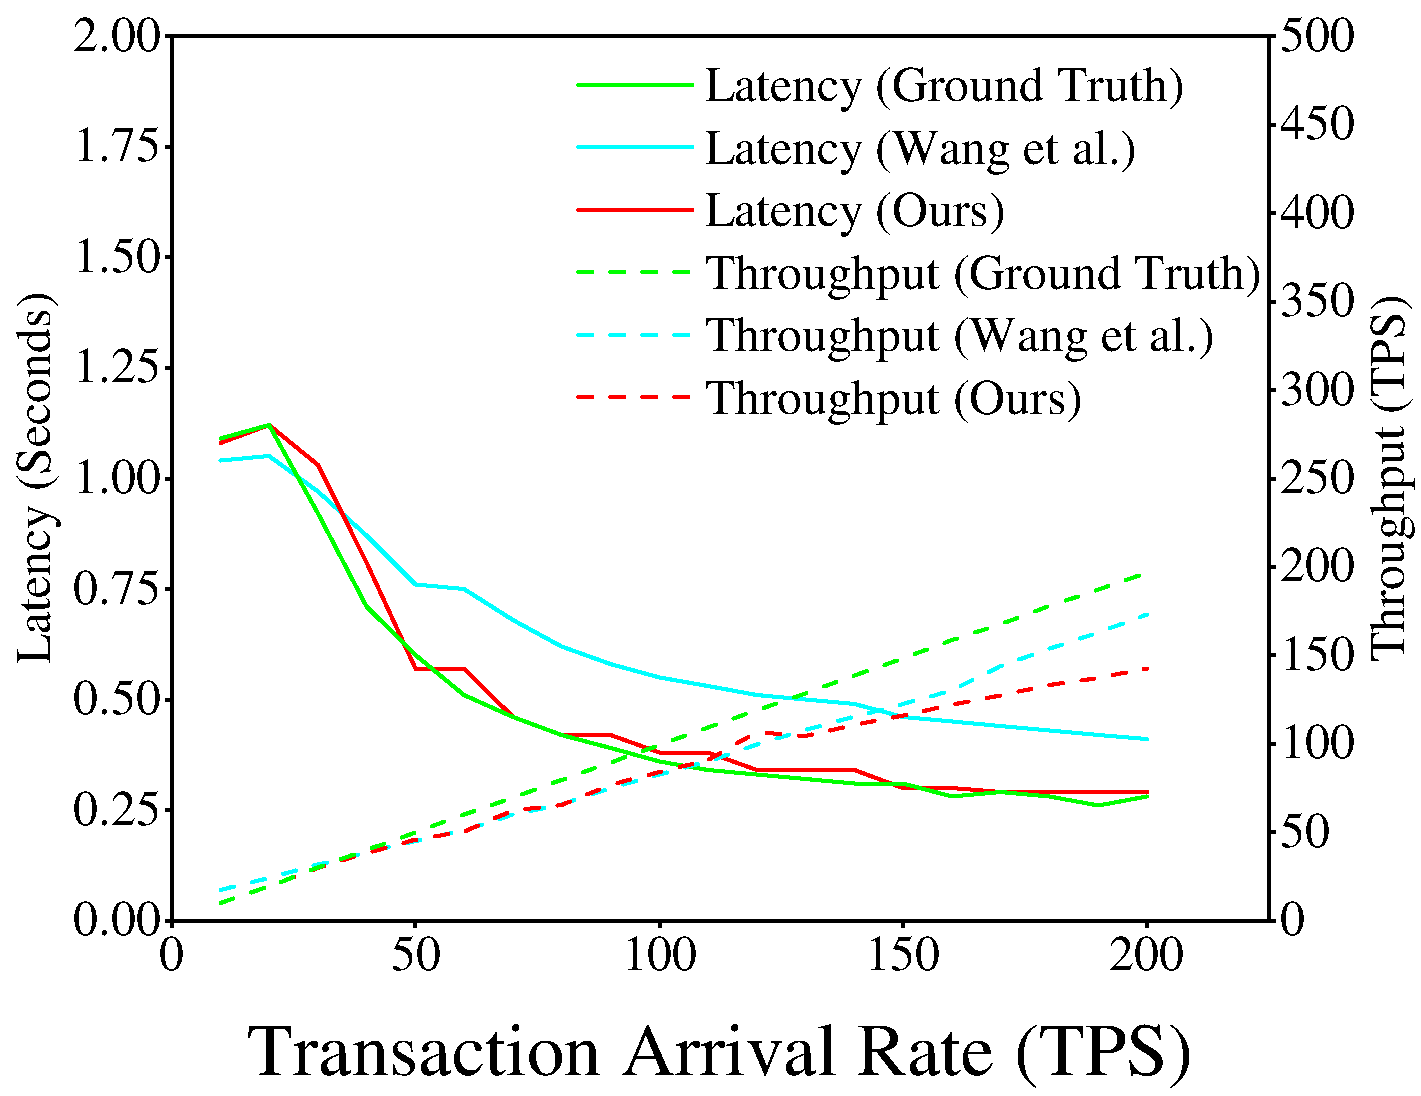
\includegraphics[width=0.35\linewidth]{figures/performance_50.pdf}
%	}
%	\hspace{0.02\linewidth} % 添加小间距
%	\subfloat[Block size = 100\label{fig:forecast_b}]{
%		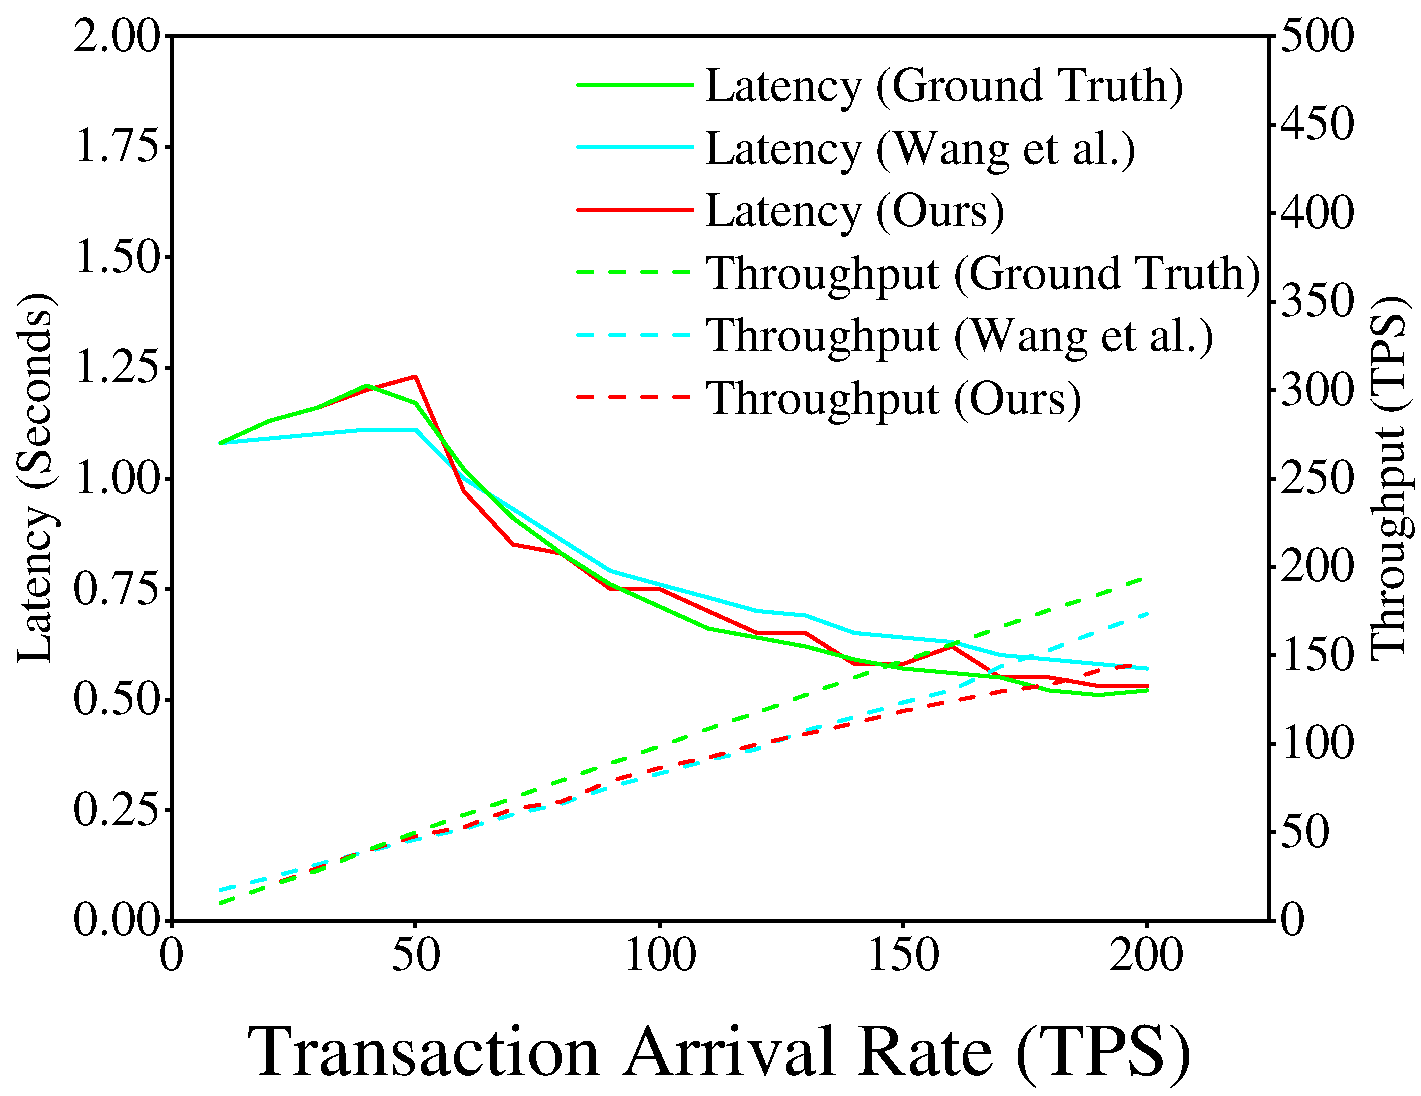
\includegraphics[width=0.35\linewidth]{figures/performance_100.pdf}
%	}
%	\\
%	\subfloat[Block size = 150\label{fig:forecast_c}]{
%		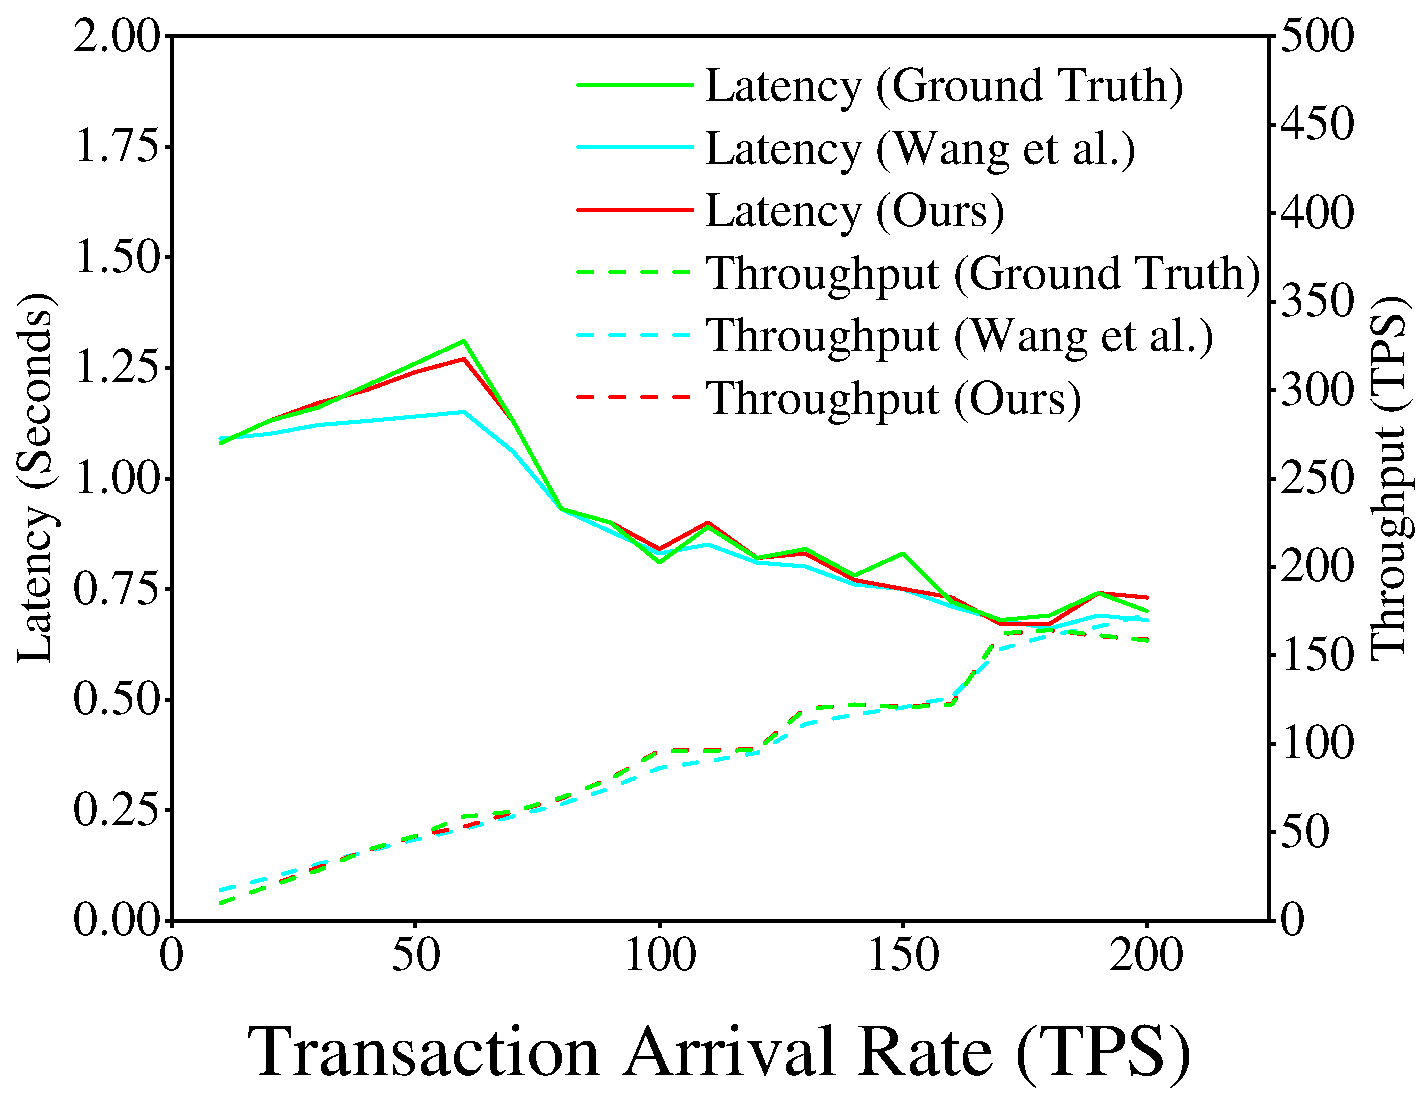
\includegraphics[width=0.35\linewidth]{figures/performance_150.pdf}
%	}
%	\hspace{0.02\linewidth} % 添加小间距
%	\subfloat[Block size = 200\label{fig:forecast_d}]{
%		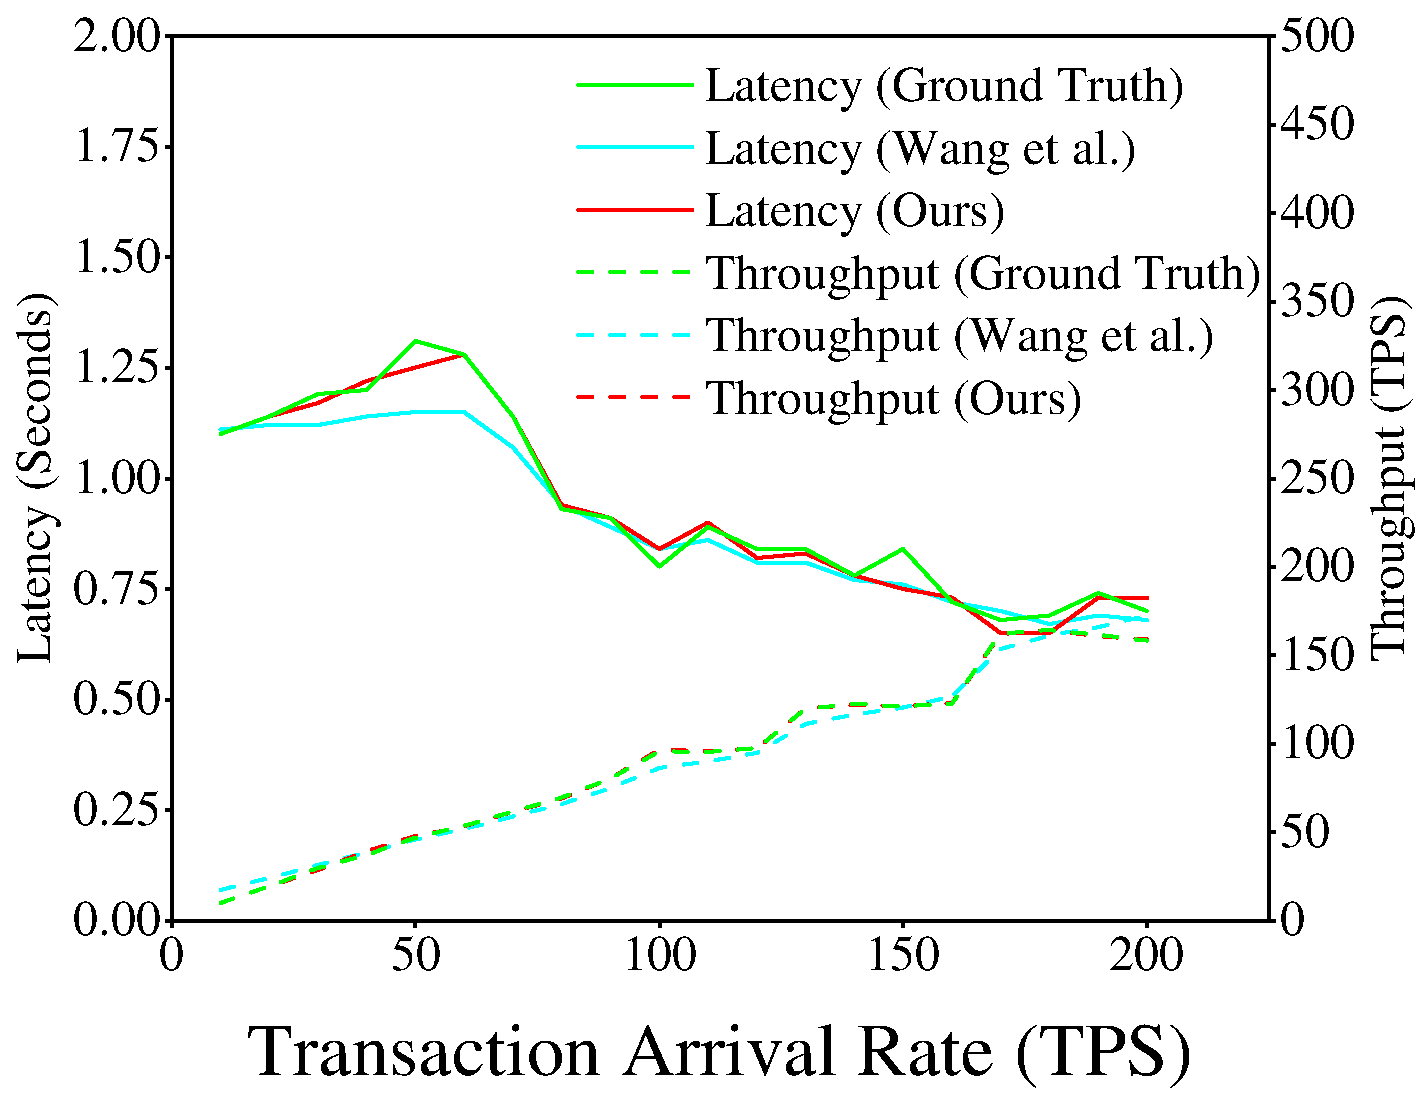
\includegraphics[width=0.35\linewidth]{figures/performance_200.pdf}
%	}
%	\caption{The latency and throughput prediction performance of the blockchain performance prediction model under different block sizes.}
%	\label{fig:performance_forecast_results}
%\end{figure*}

\begin{figure*}[t]
\centering
\subfloat [Block size = 50\label {fig:forecast_a}]{
	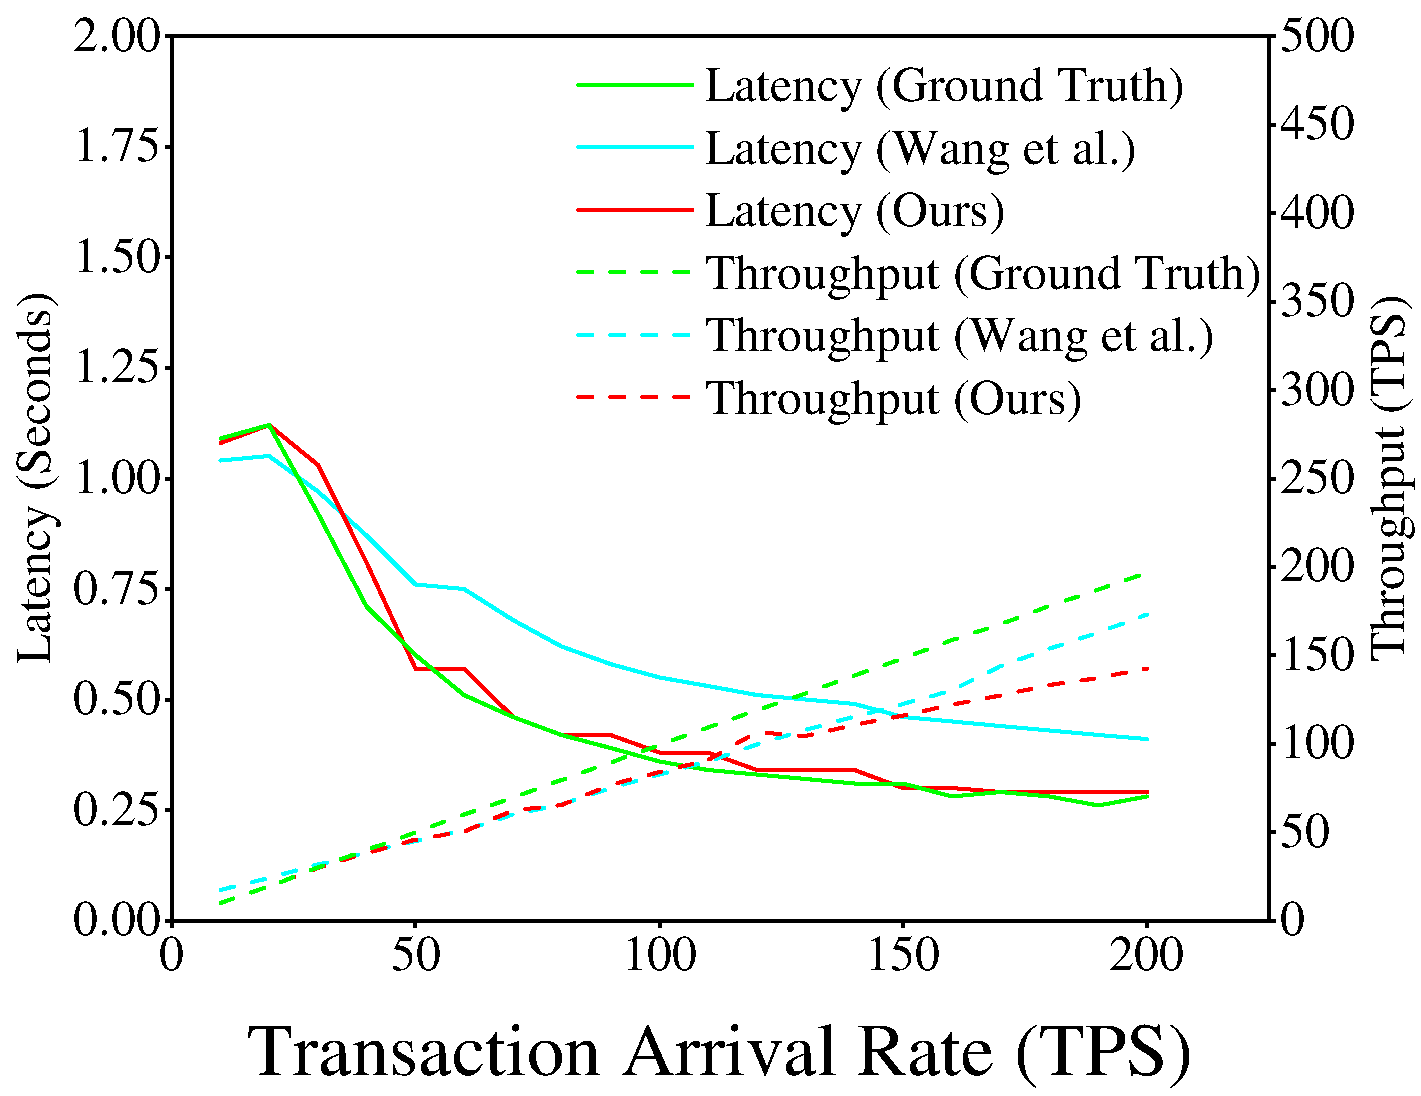
\includegraphics [width=0.22\linewidth]{figures/performance_50.pdf}
}
\hspace {0.015\linewidth} % 减小间距
\subfloat [Block size = 100\label {fig:forecast_b}]{
	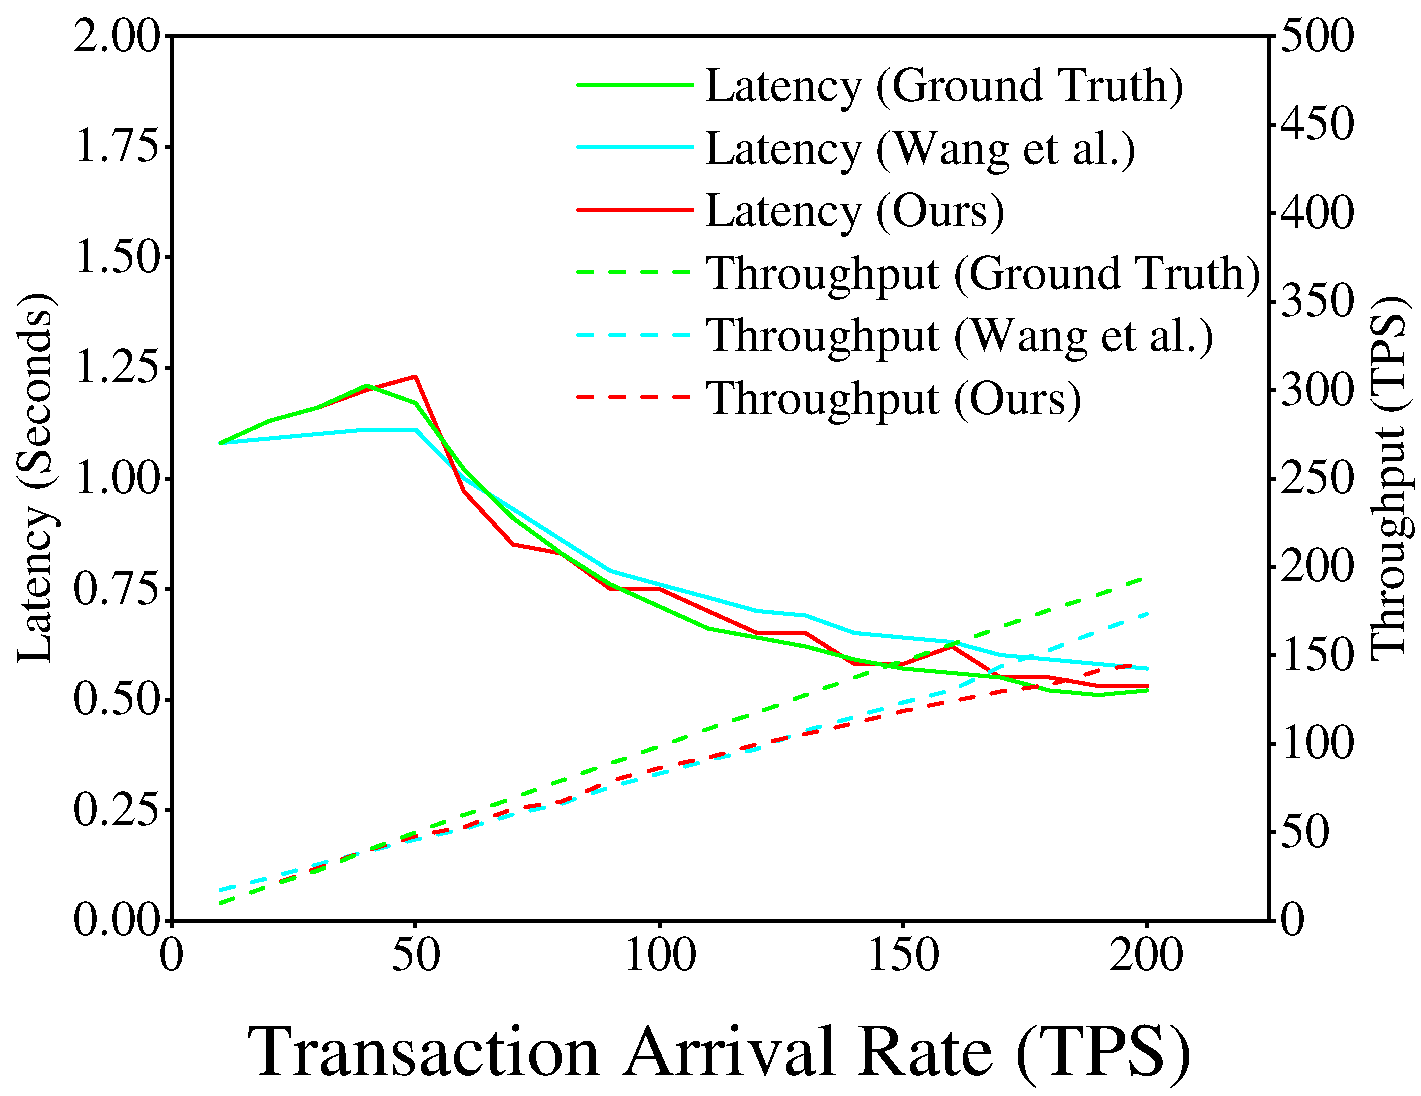
\includegraphics [width=0.22\linewidth]{figures/performance_100.pdf}
}
\hspace {0.015\linewidth} % 减小间距
\subfloat [Block size = 150\label {fig:forecast_c}]{
	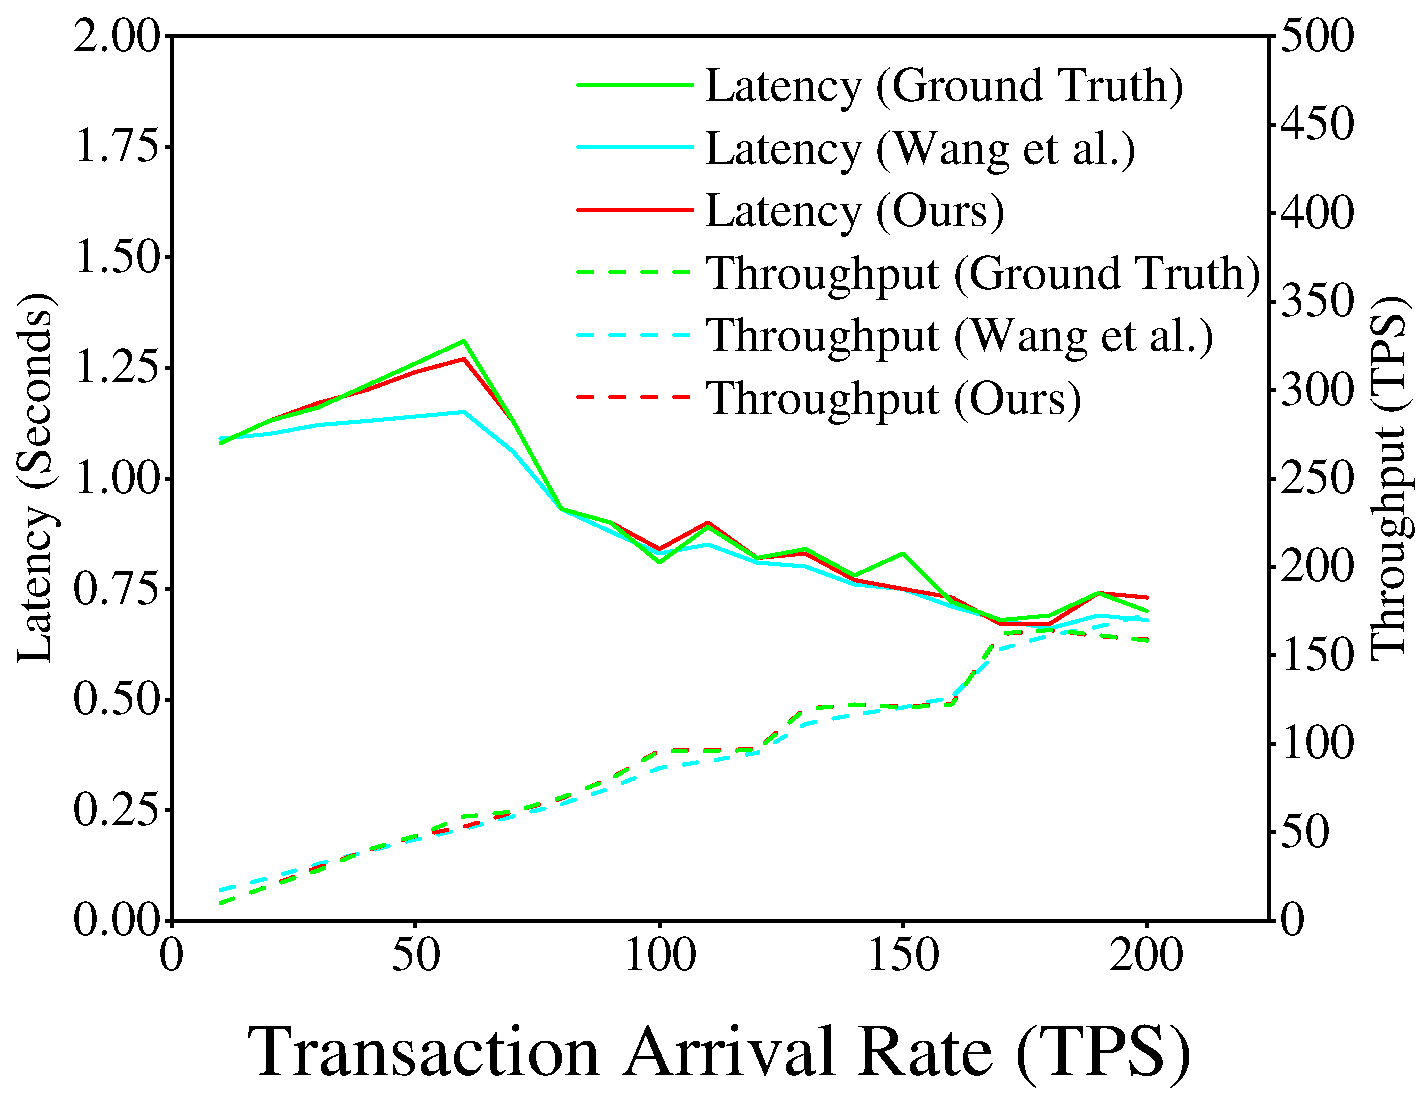
\includegraphics [width=0.22\linewidth]{figures/performance_150.pdf}
}
\hspace {0.015\linewidth} % 减小间距
\subfloat [Block size = 200\label {fig:forecast_d}]{
	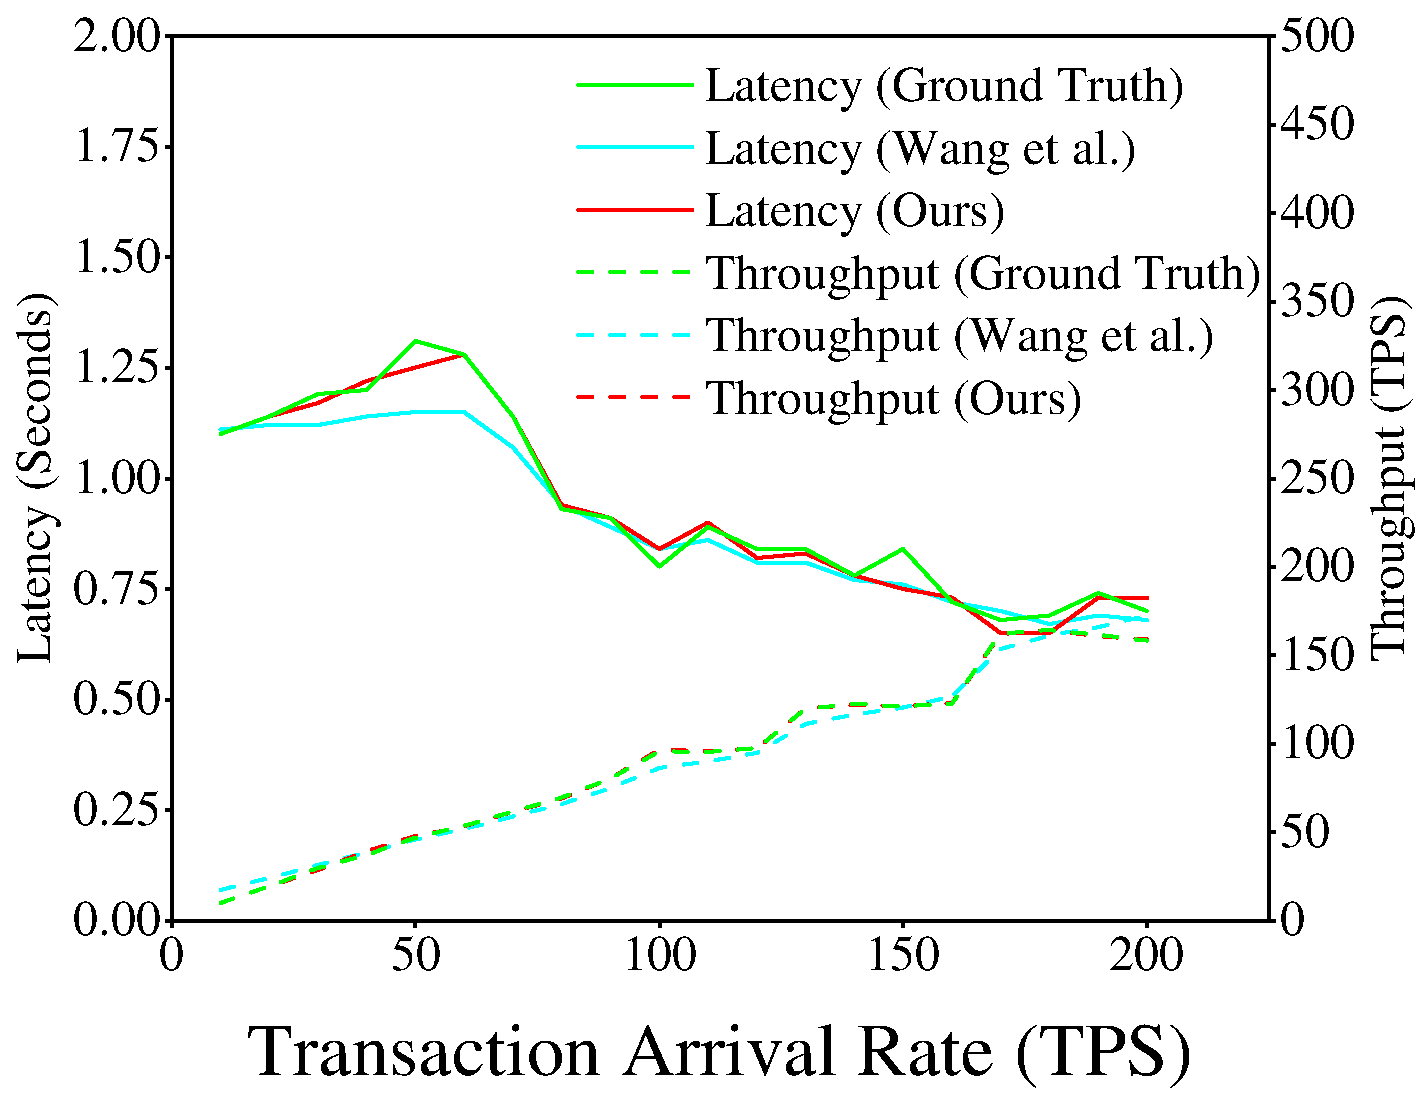
\includegraphics [width=0.22\linewidth]{figures/performance_200.pdf}
}
\caption {The latency and throughput prediction performance of the blockchain performance prediction model under different block sizes.}
\label {fig:performance_forecast_results}
\end{figure*}


\paragraph{Latency prediction}

As shown in Table~\ref{tab:performance}, the proposed model achieved the lowest latency MAPE (0.0298), with an MAE of 0.0223 and an RMSE of 0.0519. DTR achieved a lower MAE (0.0218), while the prior blockchain-oriented prediction baseline achieved a lower RMSE (0.0481). Thus, the proposed model performed best on latency MAPE, but not on MAE or RMSE.


\paragraph{Throughput prediction}

For throughput prediction, Table~\ref{tab:performance} shows that the proposed model achieved the lowest RMSE (0.0442) and MAPE (0.0037). Its MAE of 0.0167 was slightly higher than that of DTR (0.0164), although lower than those of the other evaluated baselines. The proposed model therefore performed best on throughput RMSE and MAPE, but not on MAE.

\begin{figure*}[t]
	\centering
	\subfloat[Block size = 50]{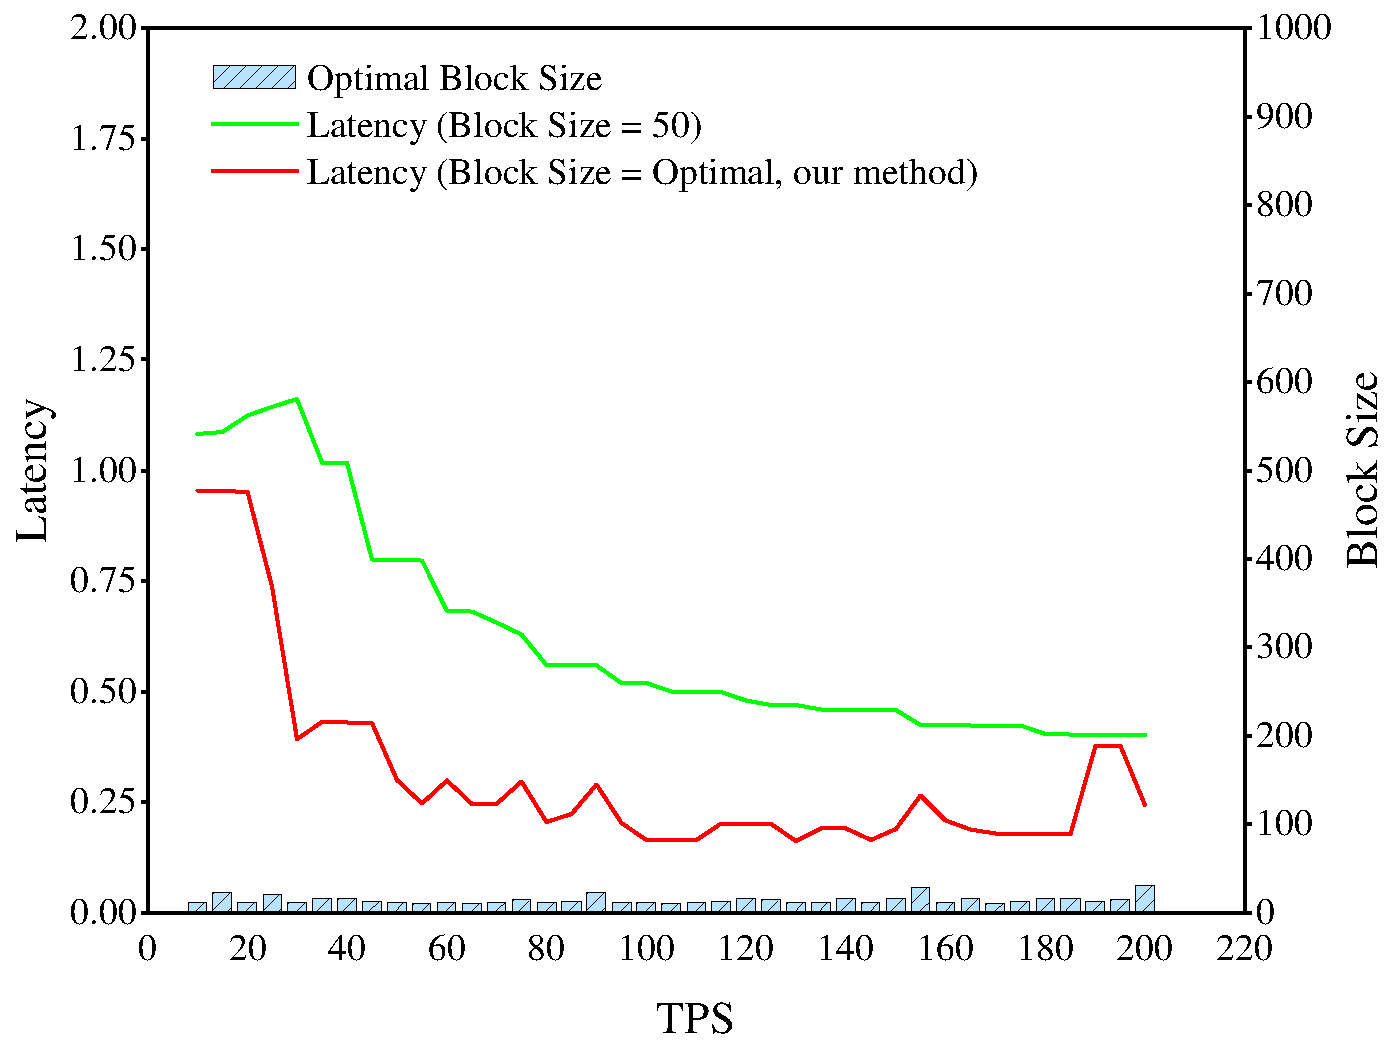
\includegraphics[width=0.4\linewidth]{figures/dw_dqn_latency_50.pdf}}
	\hspace{0.02\linewidth} % 添加小间距
	\subfloat[Block size = 100]{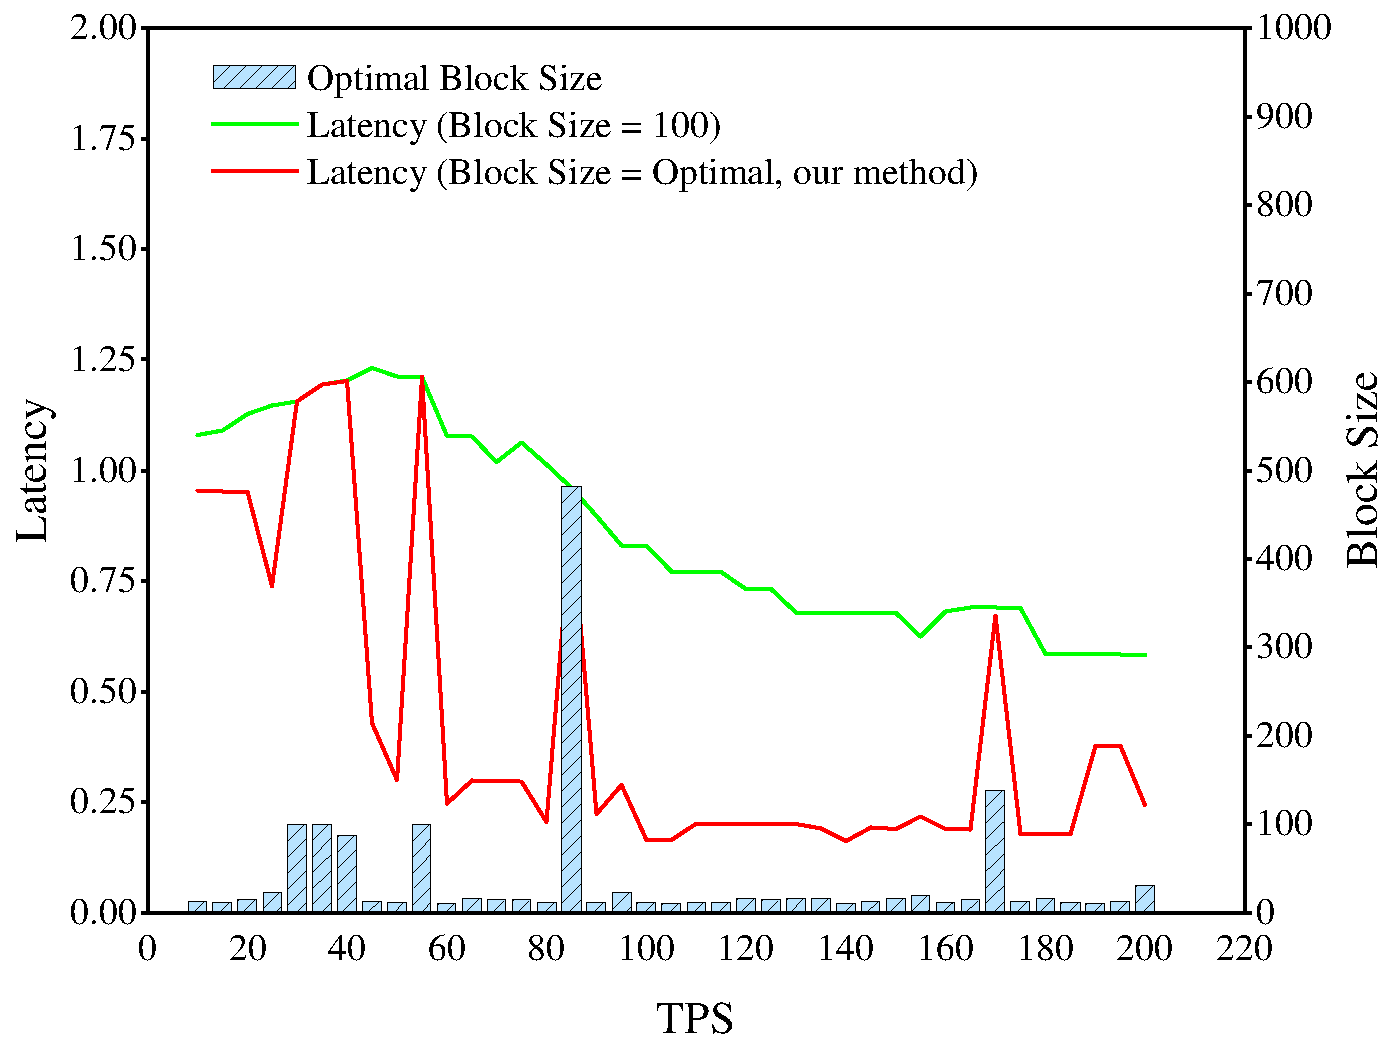
\includegraphics[width=0.4\linewidth]{figures/dw_dqn_latency_100.pdf}}
	\\[1em] % 添加垂直间距
	\subfloat[Block size = 150]{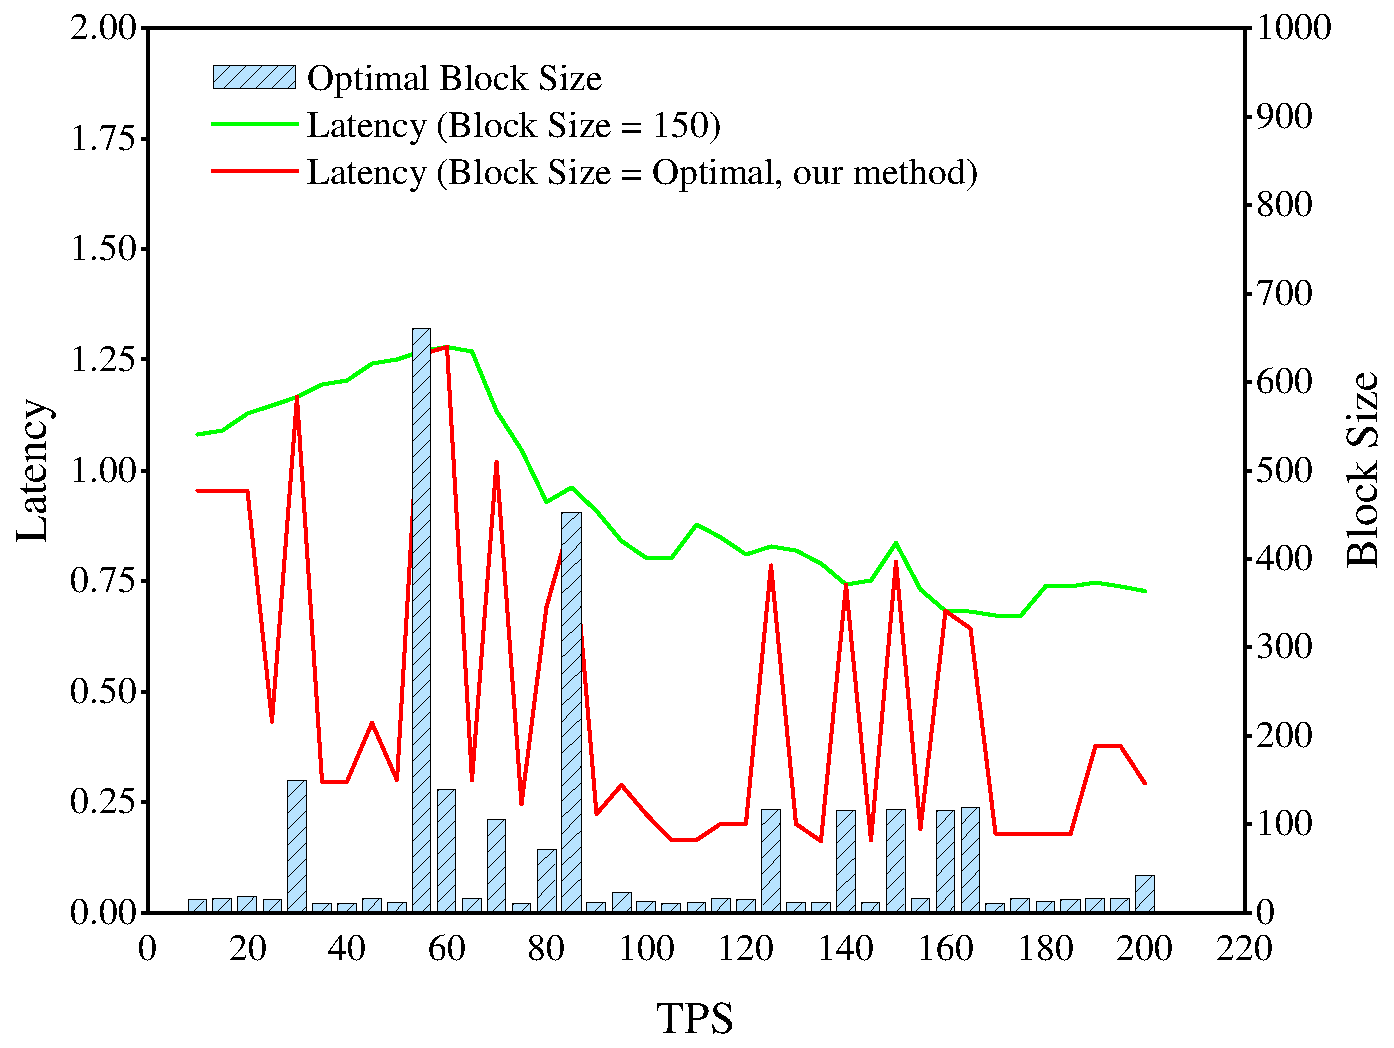
\includegraphics[width=0.4\linewidth]{figures/dw_dqn_latency_150.pdf}}
	\hspace{0.02\linewidth} % 添加小间距
	\subfloat[Block size = 200]{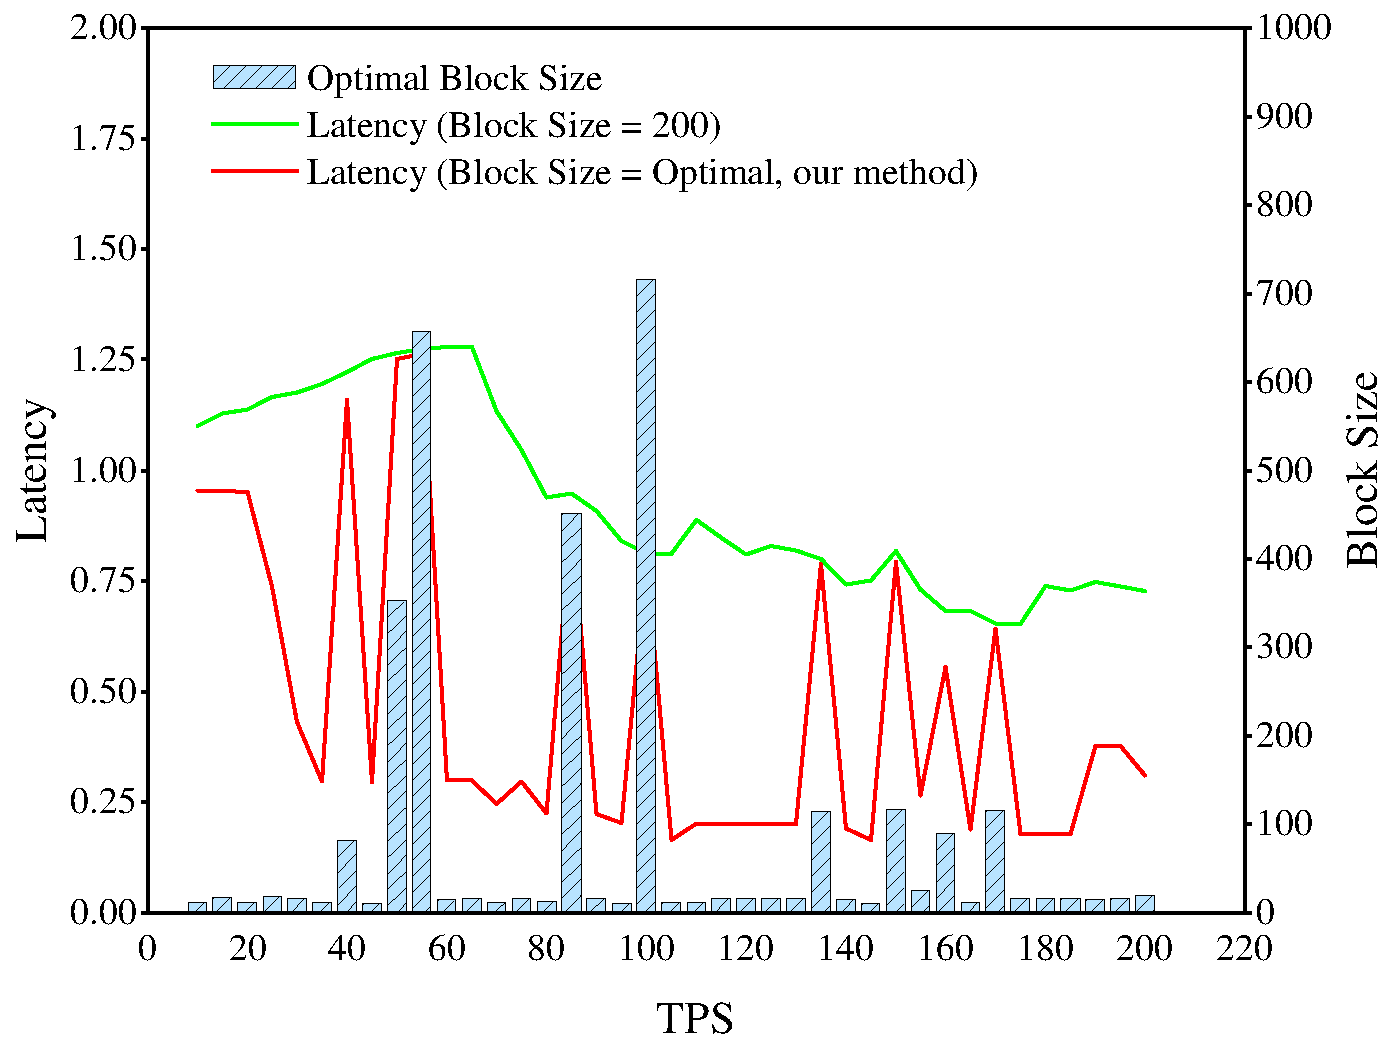
\includegraphics[width=0.4\linewidth]{figures/dw_dqn_latency_200.pdf}}
	\caption{Latency optimization under different TPS and block sizes using DW-DQN.}
	\label{fig:dw_dqn_latency}
\end{figure*}

%For smaller block sizes (50 and 100), the proposed model underestimates throughput above 140 TPS and performs worse than Wang et al.'s method, likely due to the linear performance saturation in such constrained scenarios. However, at larger block sizes (150 and 200), the throughput behavior becomes increasingly nonlinear, with obvious saturation beyond approximately 150 TPS. In these cases, the proposed model accurately captures the flattening trend, whereas Wang et al.'s method continues to underestimate throughput. This difference highlights a significant advantage of the proposed dynamic ensemble approach: the ability to adaptively select regressors that specialize in different operating regimes, allowing for accurate modeling of resource constraints and system bottlenecks.

%Table~\ref{tab:performance} clearly demonstrates our model's adaptability, as it again achieves the best overall performance in throughput prediction, with an MAE of 0.0167 and a remarkably low MAPE of 0.0037. In contrast, Wang et al.'s model produces a MAPE of 0.0973, which is more than 26 times higher. These findings support the proposed framework's ability to capture complex throughput behaviors, especially under high-load and nonlinear conditions.


%\paragraph{Summary and Insights}

%In conclusion, while the proposed model does not outperform Wang et al.'s method in all scenarios, particularly under low-capacity configurations such as block sizes of 50 and 100 for throughput prediction—its advantages become clear in more complex conditions, such as larger block sizes where nonlinear behaviors dominate. The ensemble's ability to dynamically adapt to different performance regimes, coupled with its expanded feature space and multi-objective learning formulation, provides a strong theoretical foundation for its empirical gains.

\begin{figure*}[t]
	\centering
	\subfloat[Block size = 50]{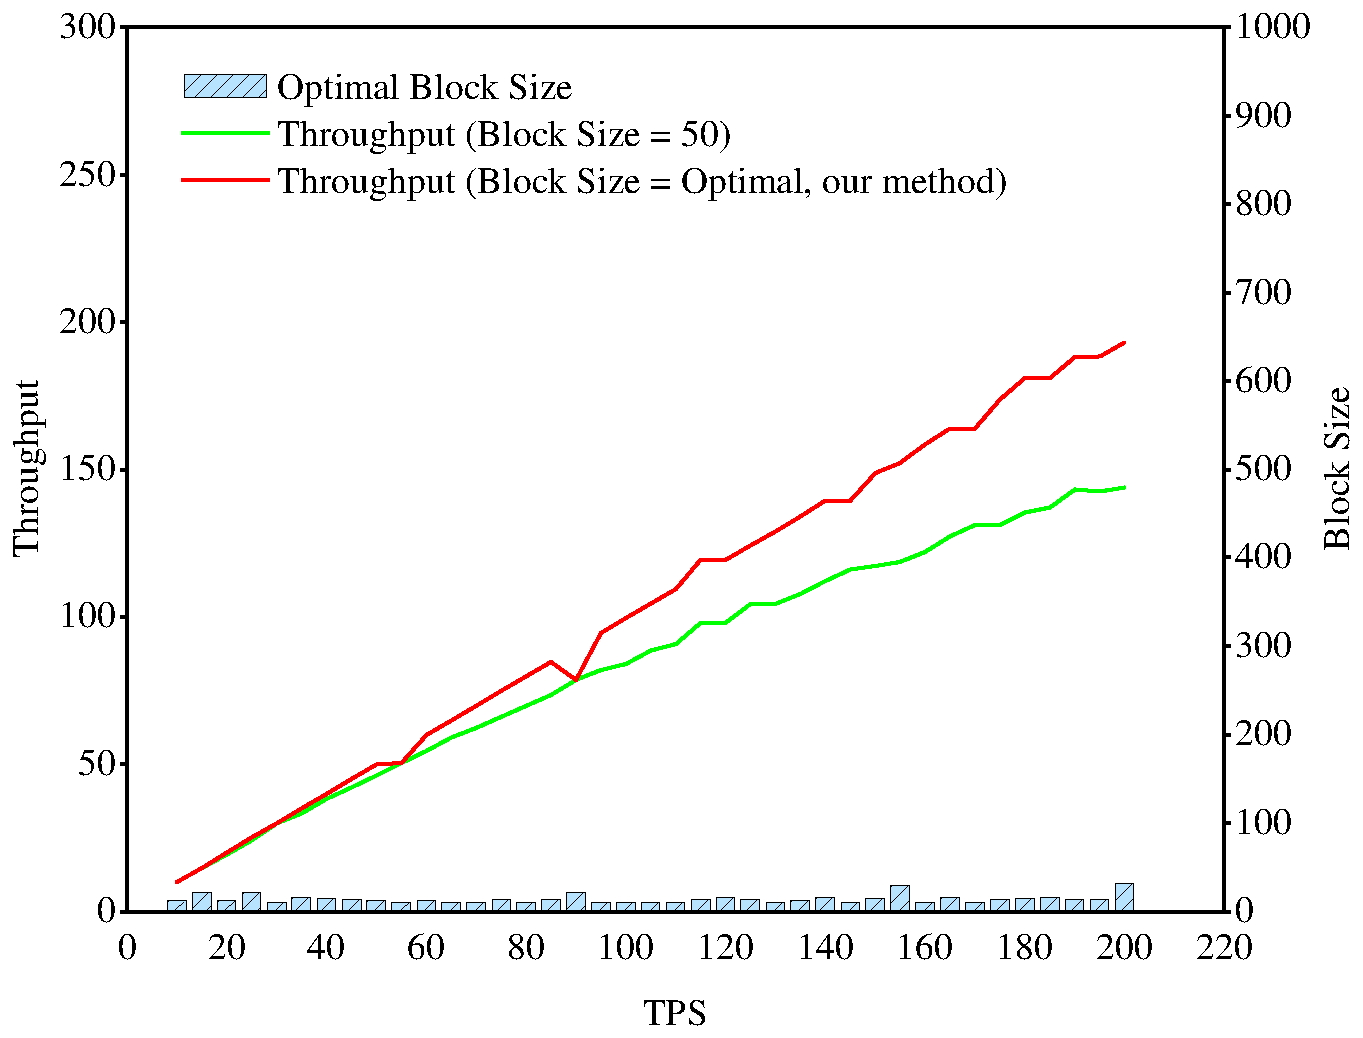
\includegraphics[width=0.4\linewidth]{figures/dw_dqn_throughput_50.pdf}}
	\hspace{0.02\linewidth} % 添加小间距
	\subfloat[Block size = 100]{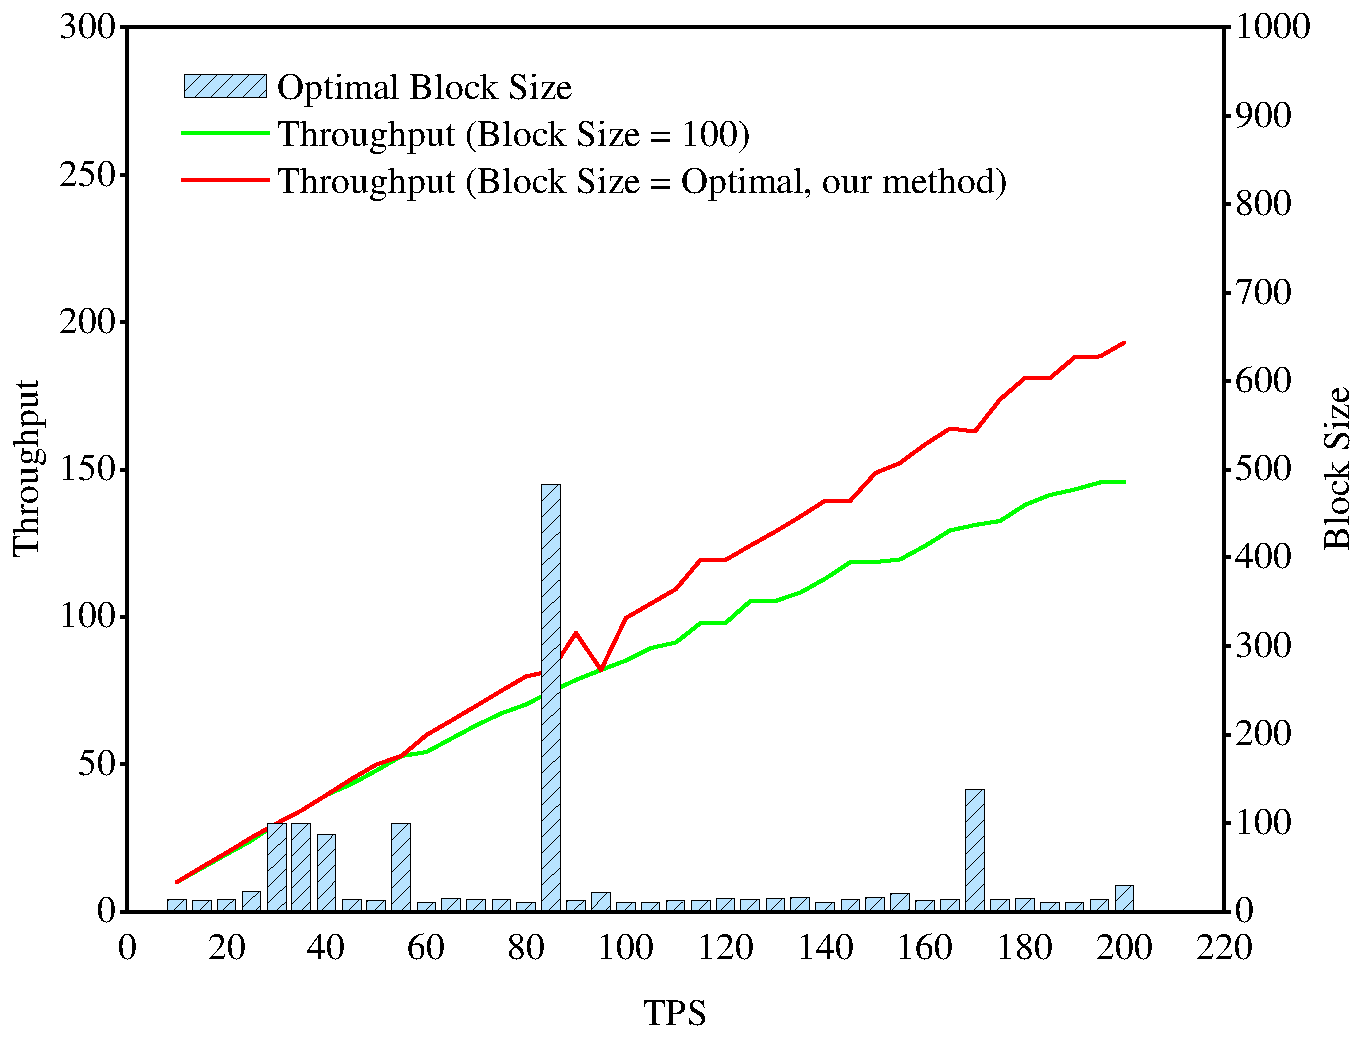
\includegraphics[width=0.4\linewidth]{figures/dw_dqn_throughput_100.pdf}}
	\\
	\subfloat[Block size = 150]{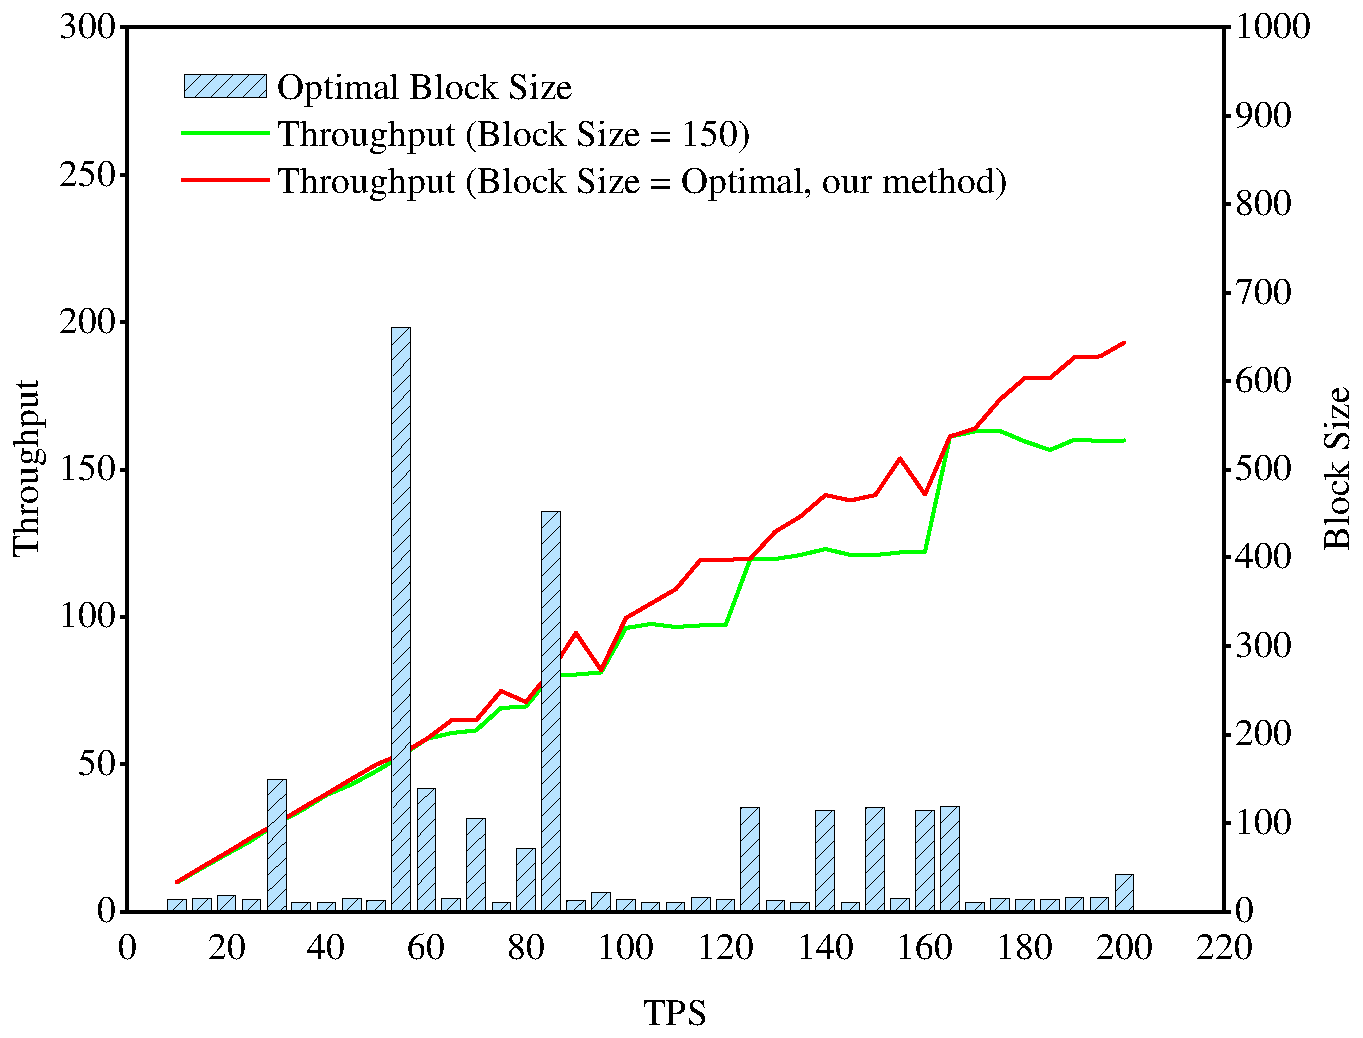
\includegraphics[width=0.4\linewidth]{figures/dw_dqn_throughput_150.pdf}}
	\hspace{0.02\linewidth} % 添加小间距
	\subfloat[Block size = 200]{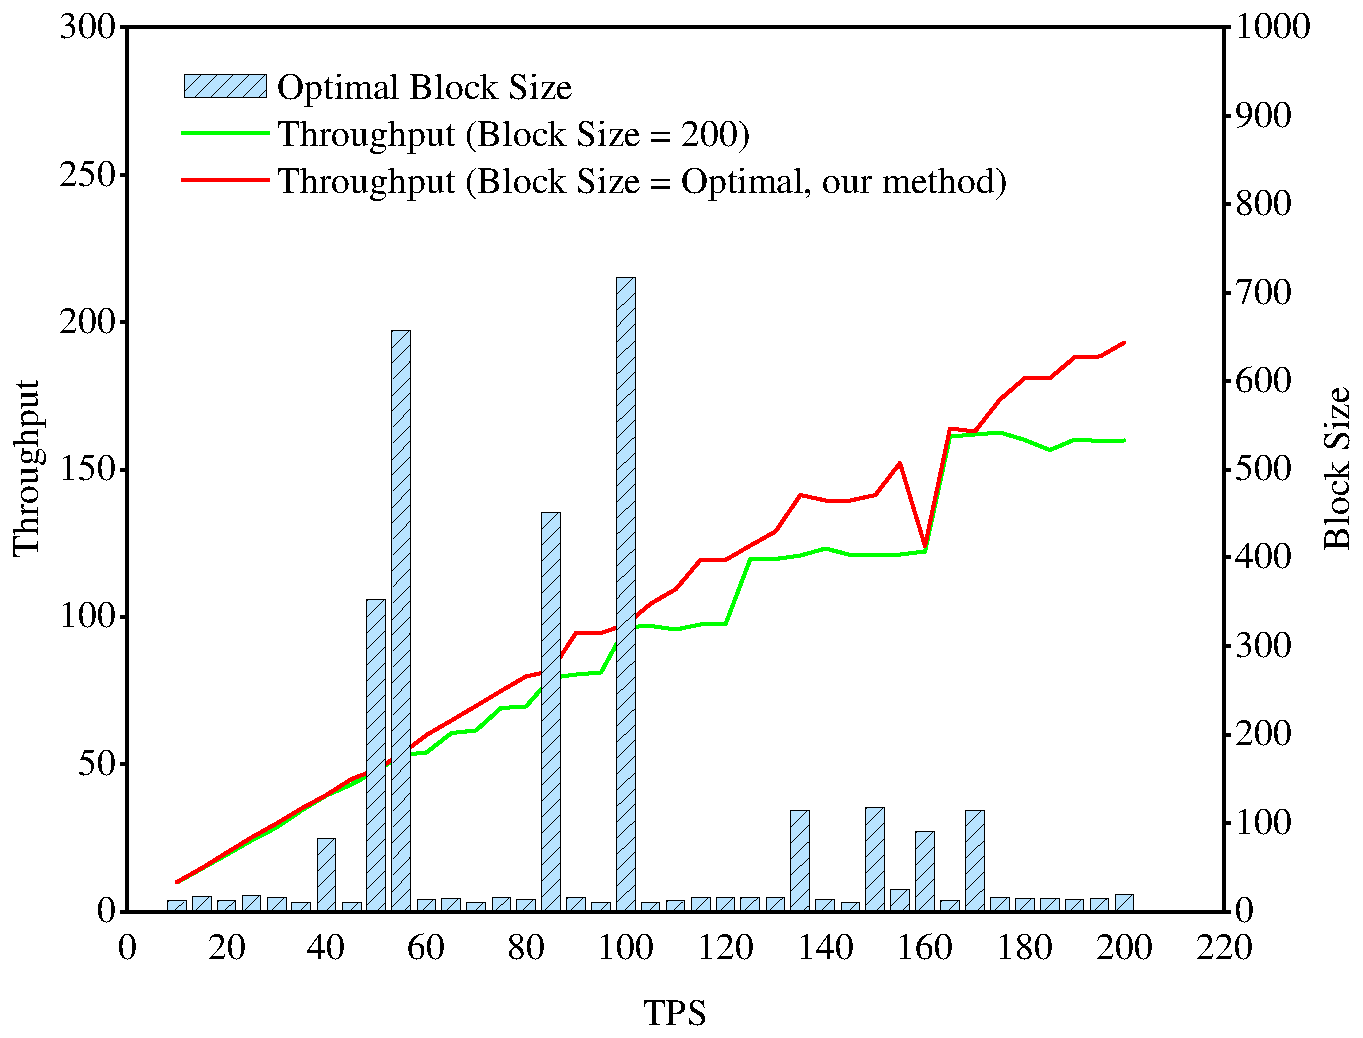
\includegraphics[width=0.4\linewidth]{figures/dw_dqn_throughput_200.pdf}}
	\caption{Throughput optimization under different TPS and block sizes using DW-DQN.}
	\label{fig:dw_dqn_throughput}
\end{figure*}

%Overall, the proposed prediction framework shows superior generalization and robustness, particularly in high-load and nonlinear scenarios. This is consistent with the visual trends shown in Figure~\ref{fig:performance_forecast_results} and supports the quantitative improvements reported in Table~\ref{tab:performance}. The model's ability to capture both early-stage linear growth and late-stage saturation behavior makes it ideal for real-time performance predicting in a variety of blockchain environments.


\subsubsection{Performance of the optimization mechanism with DW-DQN}
\vspace{6pt}
This section evaluates the proposed blockchain performance optimization mechanism based on the Dynamic Weight Deep Q-Network (DW-DQN), focusing on improvements in system latency and throughput. Experiments were conducted with four initial block sizes (50, 100, 150, and 200) under various transaction loads (TPS). The results demonstrate DW-DQN's adaptability and robustness in solving multi-objective optimization tasks.


DW-DQN consistently enhances system performance across various TPS levels, with notable improvements observed under high-load conditions. For example, when the initial block size was set to 150 and TPS increased from 60 to 140, the latency before optimization reached approximately 1.25 seconds. In contrast, DW-DQN maintained latency between 0.25 and 0.9 seconds, achieving an average improvement of 54\% (Figure~\ref{fig:dw_dqn_latency}). 
%This significant enhancement can be attributed to DW-DQN's multi-objective reward function, which dynamically adjusts weights to prioritize latency control during periods of performance degradation.

In terms of throughput, DW-DQN outperforms fixed block size baselines, especially under high TPS conditions. For example, at TPS = 160, DW-DQN achieved a maximum throughput 30\% higher than the static approach (Figure~\ref{fig:dw_dqn_throughput}). 
%This is due to DW-DQN's ability to adapt block sizes based on transaction arrival rates and processing capacity.

Tables~\ref{tab:dw_dqn_latency} and~\ref{tab:dw_dqn_throughput} summarize the optimization rates for latency and throughput, respectively. DW-DQN significantly reduced average latency and increased throughput across all initial block sizes. For example, with an initial block size of 200, latency was reduced from 0.93 seconds to 0.43 seconds (50.09\% improvement), and throughput increased from 92.37 TPS to 103.09 TPS (11.35\% improvement).


\begin{table}[!htbp]
	\centering
	\footnotesize
	\caption{The optimization rate of optimal block size on latency}
	\label{tab:dw_dqn_latency}
	\setlength{\tabcolsep}{3pt}
	\begin{tabular}{@{}l*{5}{c}@{}}
		\toprule
		\multirow{2}{*}{Metric} & \multicolumn{5}{c}{Block Size} \\
		\cmidrule(lr){2-6}
		& 50 & 100 & 150 & 200 & Optimal (Ours) \\
		\midrule
		Average Latency (s) & 0.62 & 0.87 & 0.93 & 0.93 & \textbf{0.43} \\
		Optimization Rate (\%) & 49.78 & 50.73 & 47.36 & 50.09 & — \\
		\bottomrule
	\end{tabular}
\end{table}



\begin{table}[!htbp]
	\centering
	\caption{The optimization rate of optimal block size on throughput}
	\label{tab:dw_dqn_throughput}
	\setlength{\tabcolsep}{3pt} % 缩小列间距，节省宽度
	\footnotesize
	\begin{tabular}{@{}lccccc@{}}
		\toprule
		\multirow{2}{*}{Metric} & \multicolumn{5}{c}{Block Size} \\
		\cmidrule(lr){2-6}
		& 50 & 100 & 150 & 200 & Optimal (Ours) \\
		\midrule
		\makecell[l]{Average\\Throughput (TPS)} & 84.74 & 85.74 & 92.60 & 92.37 & \textbf{103.09} \\
		Optimization Rate (\%) & 22.09 & 20.70 & 10.66 & 11.35 & — \\ % 补第5列占位横线，对齐
		\bottomrule
	\end{tabular}
\end{table}

%In summary, DW-DQN addresses key limitations of conventional DQN methods, such as fixed optimization targets and inflexible policy behaviors, through a multi-level modeling framework that improves generalization and adaptability in dynamic, high-dimensional environments. Experimental results confirm that DW-DQN can effectively adjust block sizes in real time in response to changing transaction loads, resulting in joint optimization of latency and throughput.

%Looking ahead, the proposed method is highly scalable and shows great promise for use in more complex on-chain scenarios, such as resource-aware task scheduling and adaptive tuning of consensus mechanisms. It is expected that DW-DQN will be used as an enabling technology to build highly adaptive, performance-efficient blockchain systems.

%\begin{table}[htbp]
%	\centering
%	\caption{Comparison with Related Work}
%	\label{tab:comparison}
%	\setlength{\tabcolsep}{3.5pt}
%	\footnotesize
%	\begin{tabular}{lcccccccccc}
%		\toprule
%		\multirow{3}{*}{Work} & \multicolumn{10}{c}{Criteria} \\
%		\cmidrule(lr){2-11}
%		& C1 & C2 & C3 & C4 & C5 & C6 & C7 & C8 & C9 & C10 \\
%		\midrule
%		\citep{jamil2022improving} & $\checkmark$ & $\checkmark$ & $\checkmark$ & $\checkmark$ & $\times$ & $\times$ & $*$ & $\times$ & $\times$ & $\times$ \\
%		\citep{chen2022latency} & 
%		$\times$ & $\times$ & $\checkmark$ & $\times$ & $\checkmark$ & $\times$ & $*$ & $\times$ & $\times$ & $\times$ \\
%		\citep{wilhelmi2022end} & $\times$ & $\times$ & $\checkmark$ & $\times$ & $\checkmark$ & $\times$ & $*$ & $\times$ & $\times$ & $\times$ \\
%		\citep{wang2022bpr} & $\checkmark$ & $\checkmark$ & $\checkmark$ & $\times$ & $\checkmark$ & $\checkmark$ & $\times$ & $\times$ & $\times$ & $\times$ \\
%		\citep{wang2023learningchain} & $\checkmark$ & $\checkmark$ & $\checkmark$ & $\checkmark$ & $\checkmark$ & $\checkmark$ & $\checkmark$ & $\checkmark$ & $\times$ & $\times$ \\
%		\textbf{Ours} & $\checkmark$ & $\checkmark$ & $\checkmark$ & $\checkmark$ & $\checkmark$ & $\checkmark$ & $\checkmark$ & $\checkmark$ & $\checkmark$ & $\checkmark$ \\
%		\bottomrule
%	\end{tabular}
	
%	\vspace{0.2cm}
%	\footnotesize
%	\begin{tabular}{ll}
%		C1: & Platform-agnostic (not limited to specific blockchain platforms) \\
%		C2: & Throughput optimization \\
%		C3: & Latency optimization \\
%		C4: & High scalability and generalization \\
%		C5: & Open-sourced code availability \\
%		C6: & Public blockchain performance dataset availability \\
%		C7: & Effective under few-shot (small sample) scenarios \\
%		C8: & End-to-end integrated framework (prediction + optimization) \\
%		C9: & Adaptive to dynamic workload and network changes \\
%		C10: & Multi-objective optimization capability (e.g., throughput + latency) \\
%	\end{tabular}
	
%	\smallskip
%	\textit{Note:} $\checkmark$ denotes ``Yes'', $\times$ denotes ``No'', and $*$ denotes ``Unknown / Not specified''.
%\end{table}


\subsection{Ablation study}
\vspace{6pt}
To evaluate the contribution of individual components within ChainOptNet, we conducted an ablation study on the HFBDP dataset. The complete optimization pipeline was retained, while one key component was removed or replaced at a time. Specifically, the CFAD module was replaced with a standard LSTM predictor, the ensemble prediction framework was replaced with the best-performing individual predictor, and the dynamic weighting mechanism was replaced with a fixed-weight reward design. The optimization performance was evaluated using average latency and average throughput over all tested workload scenarios.

To ensure a fair comparison, all ablation variants were evaluated under the same HFBDP workload traces, blockchain configurations, and optimization settings. The reported results correspond to the average performance across all tested transaction arrival rates (TPS) and initial block-size settings.

\begin{table}[!htbp]
	\centering
	\footnotesize
	\caption{Ablation study results on the HFBDP dataset}
	\label{tab:ablation_study}
	\setlength{\tabcolsep}{6pt}
	\begin{tabular}{@{}lcc@{}}
		\toprule
		Model & \shortstack{Average Latency \\ (s)} & \shortstack{Average Throughput \\ (TPS)} \\
		\midrule
		Full ChainOptNet & \textbf{0.43} & \textbf{103.09} \\
		w/o CFAD & 0.49 & 98.37 \\
		w/o Ensemble Prediction & 0.47 & 99.82 \\
		w/o Dynamic Weighting & 0.58 & 93.74 \\
		\bottomrule
	\end{tabular}
\end{table}

As shown in Table~\ref{tab:ablation_study}, removing the CFAD module leads to noticeable performance degradation. The average latency increases from 0.43~s to 0.49~s, while the average throughput decreases from 103.09 TPS to 98.37 TPS. This result indicates that accurate transaction arrival rate prediction is essential for effective block-size optimization.

Replacing the ensemble prediction framework with a single predictor also reduces optimization performance. Although the degradation is less severe than removing CFAD, the increase in latency and decrease in throughput demonstrate the importance of combining heterogeneous prediction models. The inverse-error-weighted ensemble strategy improves prediction robustness and provides more reliable performance estimates for the optimization module.

The most significant performance degradation is observed when the dynamic weighting mechanism is removed from DW-DQN. In this case, the average latency increases to 0.58~s and the average throughput drops to 93.74 TPS. This finding confirms that adaptive reward balancing plays a critical role in maintaining an effective trade-off between latency and throughput under varying workload conditions.

Overall, the results validate the necessity and complementary effectiveness of the three major components in ChainOptNet. CFAD provides accurate workload forecasting, the ensemble prediction framework improves blockchain performance estimation, and the dynamic weighting mechanism enables adaptive multi-objective optimization. Together, these components contribute to the superior performance achieved by the proposed framework.

\begin{figure*}[t]
	\centering
	\subfloat[Latency vs. Discount Factor]{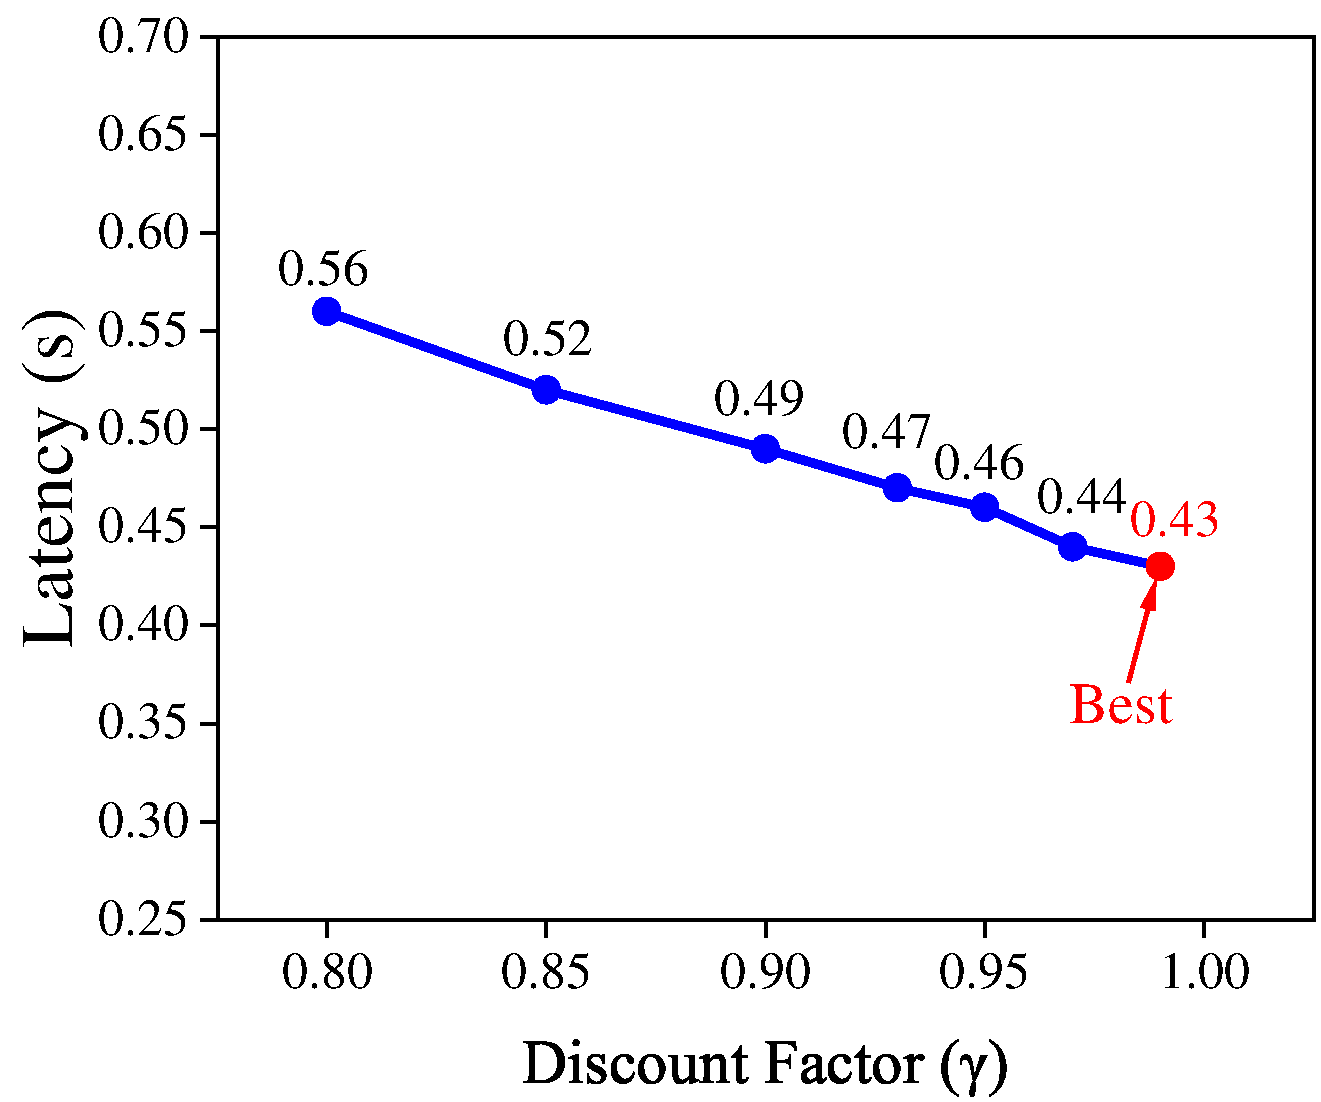
\includegraphics[width=0.22\linewidth]{figures/hy_1.pdf}}
	\hspace{0.015\linewidth}
	\subfloat[Throughput vs. Discount Factor]{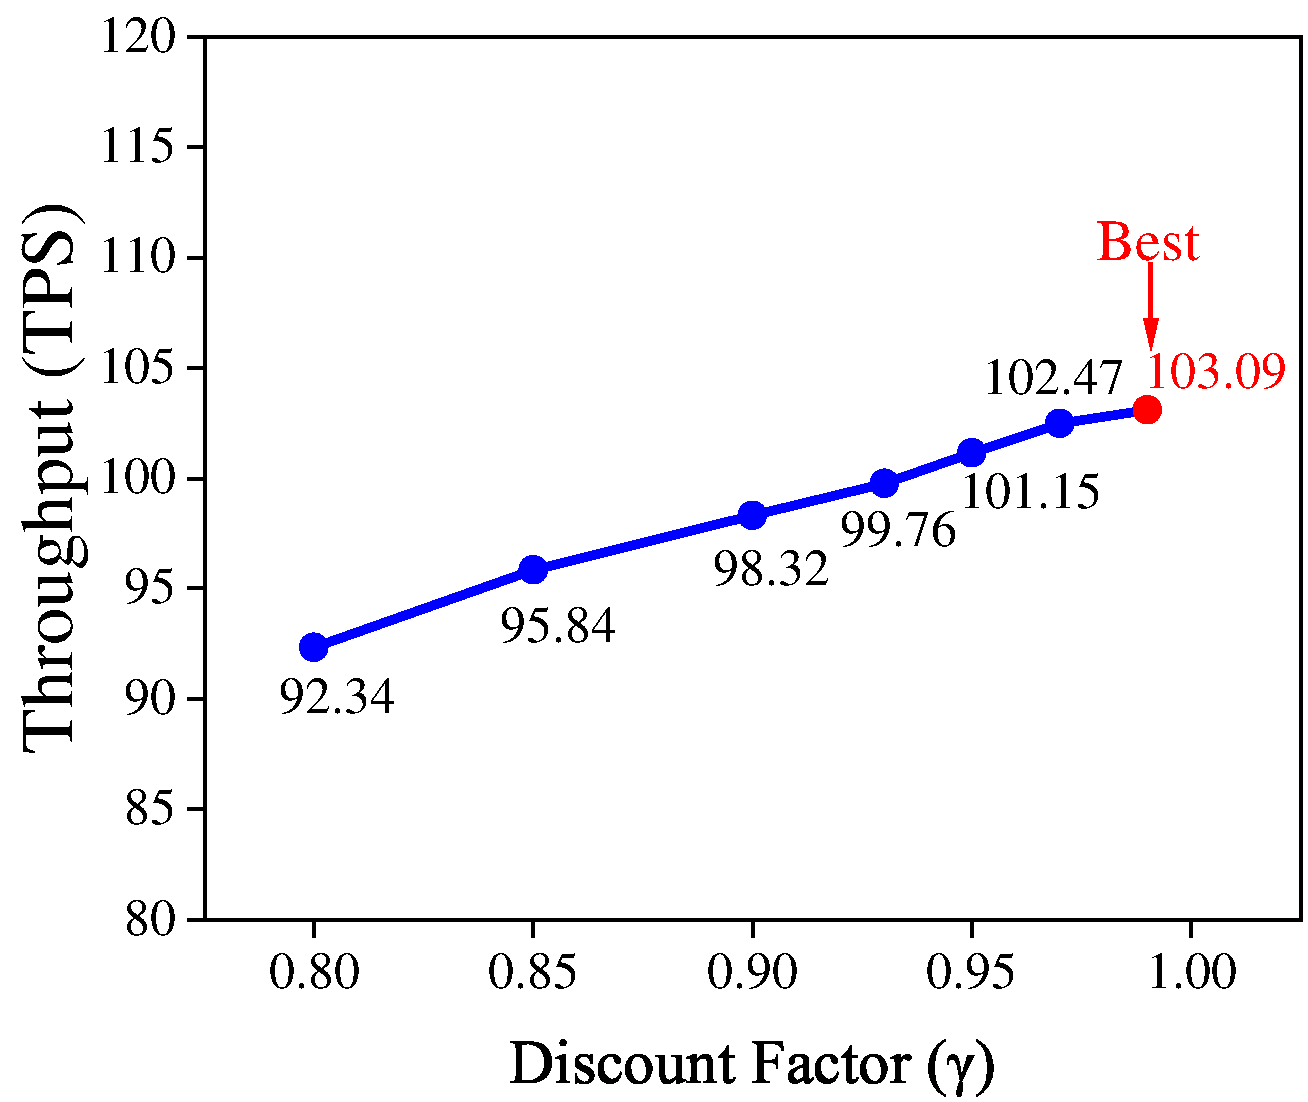
\includegraphics[width=0.22\linewidth]{figures/hy_2.pdf}}
	\hspace{0.015\linewidth}
	\subfloat[Latency vs. Replay Buffer Size]{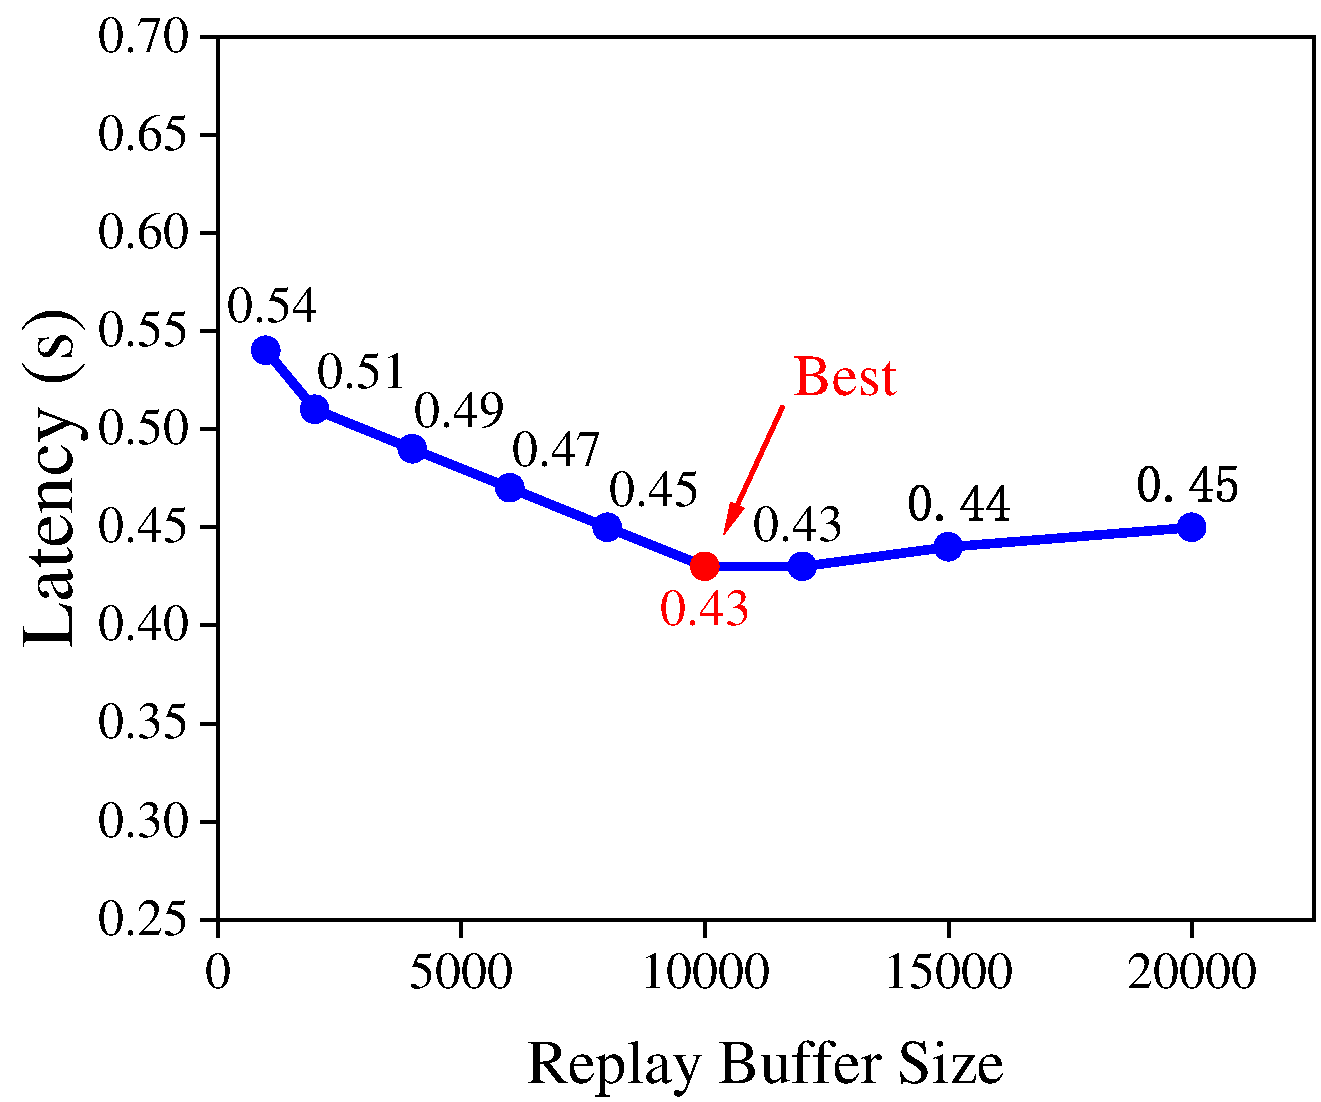
\includegraphics[width=0.22\linewidth]{figures/hy_3.pdf}}
	\hspace{0.015\linewidth}
	\subfloat[Throughput vs. Replay Buffer Size]{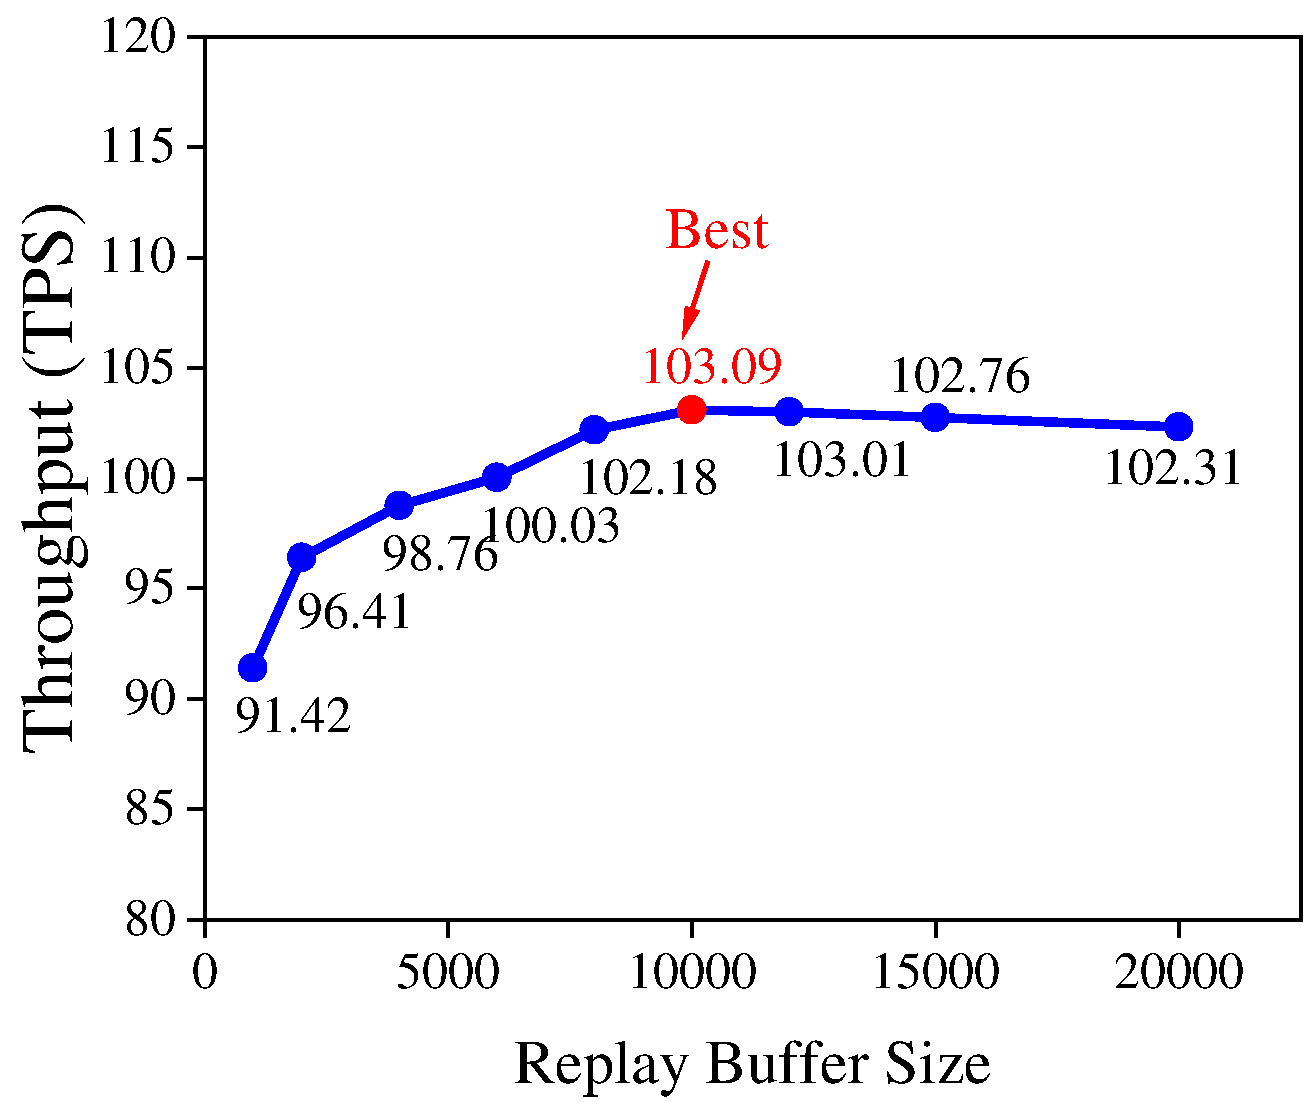
\includegraphics[width=0.22\linewidth]{figures/hy_4.pdf}}
	\caption{Sensitivity analysis of DW-DQN hyperparameters. (a) and (b) show the impact of discount factor on latency and throughput, respectively. (c) and (d) show the impact of replay buffer size on latency and throughput, respectively.}
	\label{fig:hyperparameter_analysis}
\end{figure*}

\subsection{Hyperparameter analysis}
\vspace{6pt}
\begin{table}[!htbp]
	\centering
	\caption{Sensitivity analysis of DW-DQN hyperparameters.}
	\label{tab:hyperparameter_analysis}
	\setlength{\tabcolsep}{6pt}
	\begin{tabular}{@{}lccc@{}}
		\toprule
		Parameter & Value & Latency (s) & Throughput (TPS) \\
		\midrule
		$\gamma$ & 0.80 & 0.56 & 92.34 \\
		$\gamma$ & 0.85 & 0.52 & 95.84 \\
		$\gamma$ & 0.90 & 0.49 & 98.32 \\
		$\gamma$ & 0.93 & 0.47 & 99.76 \\
		$\gamma$ & 0.95 & 0.46 & 101.15 \\
		$\gamma$ & 0.97 & 0.44 & 102.47 \\
		$\gamma$ & \textbf{0.99} & \textbf{0.43} & \textbf{103.09} \\
		\midrule
		Replay Buffer & 1000 & 0.54 & 94.12 \\
		Replay Buffer & 2000 & 0.51 & 96.41 \\
		Replay Buffer & 4000 & 0.49 & 98.76 \\
		Replay Buffer & 6000 & 0.47 & 100.03 \\
		Replay Buffer & 8000 & 0.45 & 102.18 \\
		Replay Buffer & \textbf{10000} & \textbf{0.43} & \textbf{103.09} \\
		Replay Buffer & 12000 & 0.43 & 103.01 \\
		Replay Buffer & 15000 & 0.44 & 102.76 \\
		Replay Buffer & 20000 & 0.45 & 102.31 \\
		\bottomrule
	\end{tabular}
\end{table}
To investigate the sensitivity of the proposed optimization framework to key DW-DQN hyperparameters, we conducted a comprehensive sensitivity analysis by varying the discount factor and replay buffer size on the HFBDP dataset. The corresponding latency and throughput obtained under different parameter settings are summarized in Table~\ref{tab:hyperparameter_analysis}, while the variation trends are illustrated in Fig.~\ref{fig:hyperparameter_analysis}.

\textbf{Discount factor ($\gamma$).}
The discount factor determines the importance of future rewards during policy learning. As shown in Table~\ref{tab:hyperparameter_analysis}, the optimization performance improves steadily as $\gamma$ increases from 0.80 to 0.99. Specifically, the average latency decreases from 0.56~s to 0.43~s, while the average throughput increases from 92.34 TPS to 103.09 TPS. When $\gamma$ is relatively small, the agent mainly focuses on immediate rewards, resulting in conservative block-size adjustment decisions and relatively lower optimization performance. As $\gamma$ increases beyond 0.93, the agent gradually learns more effective long-term optimization policies, leading to noticeable reductions in latency and continuous improvements in throughput. The best optimization performance is achieved when $\gamma=0.99$, indicating that emphasizing long-term cumulative rewards is beneficial for dynamic blockchain parameter optimization.

\textbf{Replay buffer size.}
The replay buffer size controls the number of historical experiences used for network updates. As the replay buffer size increases from 1000 to 10000, both latency and throughput are continuously improved. In particular, the average latency decreases from 0.54~s to 0.43~s, while the throughput increases from 94.12 TPS to 103.09 TPS. This improvement demonstrates that a larger replay buffer provides more diverse training samples, thereby improving policy stability and convergence. However, when the replay buffer size exceeds 10000, the performance gain becomes marginal. Although the replay buffer continues to increase to 12000, 15000, and 20000, the throughput remains almost unchanged while the latency exhibits a slight increase. This observation suggests that excessively large replay memories introduce additional storage overhead without providing significant improvements in optimization performance.

Overall, the proposed DW-DQN framework demonstrates stable optimization performance under different hyperparameter settings. Both the discount factor and replay buffer size exhibit clear convergence trends, indicating that the proposed optimization strategy is relatively robust to hyperparameter variations. Based on the above analysis, a discount factor of 0.99 and a replay buffer size of 10000 are selected for all subsequent experiments, as they provide the best trade-off between optimization effectiveness and computational efficiency.



\subsection{Comparative analysis}
\vspace{6pt}

Figure~\ref{fig:comparison_latency} shows that the proposed DW-DQN method consistently outperforms representative prediction-driven, score-based optimization methods across varying transaction loads, particularly under high-TPS conditions. As TPS increases, the latency reduction achieved by this class of baselines gradually plateaus, whereas DW-DQN continues to reduce latency significantly. For example, at TPS = 200, DW-DQN achieves a substantial latency reduction compared with the reference score-based strategy, demonstrating superior adaptability to performance degradation under heavy workloads.

\begin{figure}
	\centering
	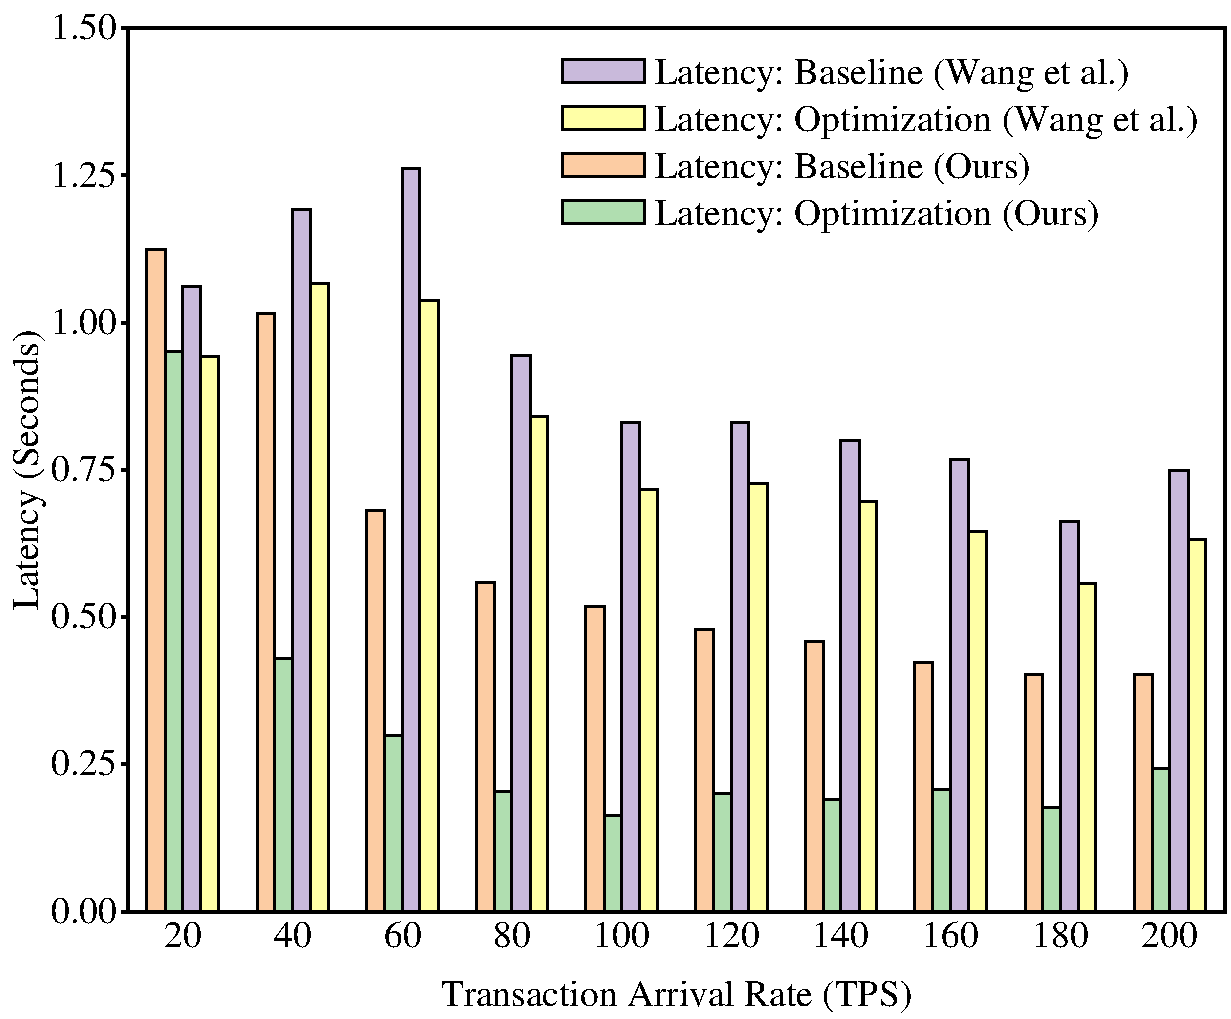
\includegraphics[width=.9\columnwidth]{figures/comparison_latency.pdf}
	\caption{Latency comparison under different TPS.}
	\label{fig:comparison_latency}
\end{figure}
As the transaction load increases, the performance gap between DW-DQN and the score-based baselines becomes increasingly evident. Under low-load conditions, both types of methods achieve relatively low latency since the blockchain network is not heavily congested. However, as TPS exceeds 120, score-based strategies gradually lose their ability to effectively adapt to rapidly changing workloads, resulting in a noticeable increase in latency. In contrast, DW-DQN maintains consistently lower latency by continuously adjusting the block size according to the current network state, demonstrating stronger adaptability under dynamic blockchain environments.

Figure~\ref{fig:comparison_throughput} further illustrates that DW-DQN consistently achieves higher throughput than the score-based baselines across all tested TPS levels, with particularly noticeable improvements under medium- and high-load scenarios (TPS $>$ 100). For instance, at TPS = 180 and TPS = 200, DW-DQN improves throughput by approximately 25 TPS compared with the reference score-based strategy, demonstrating better scalability in transaction-intensive environments.

\begin{figure}
	\centering
	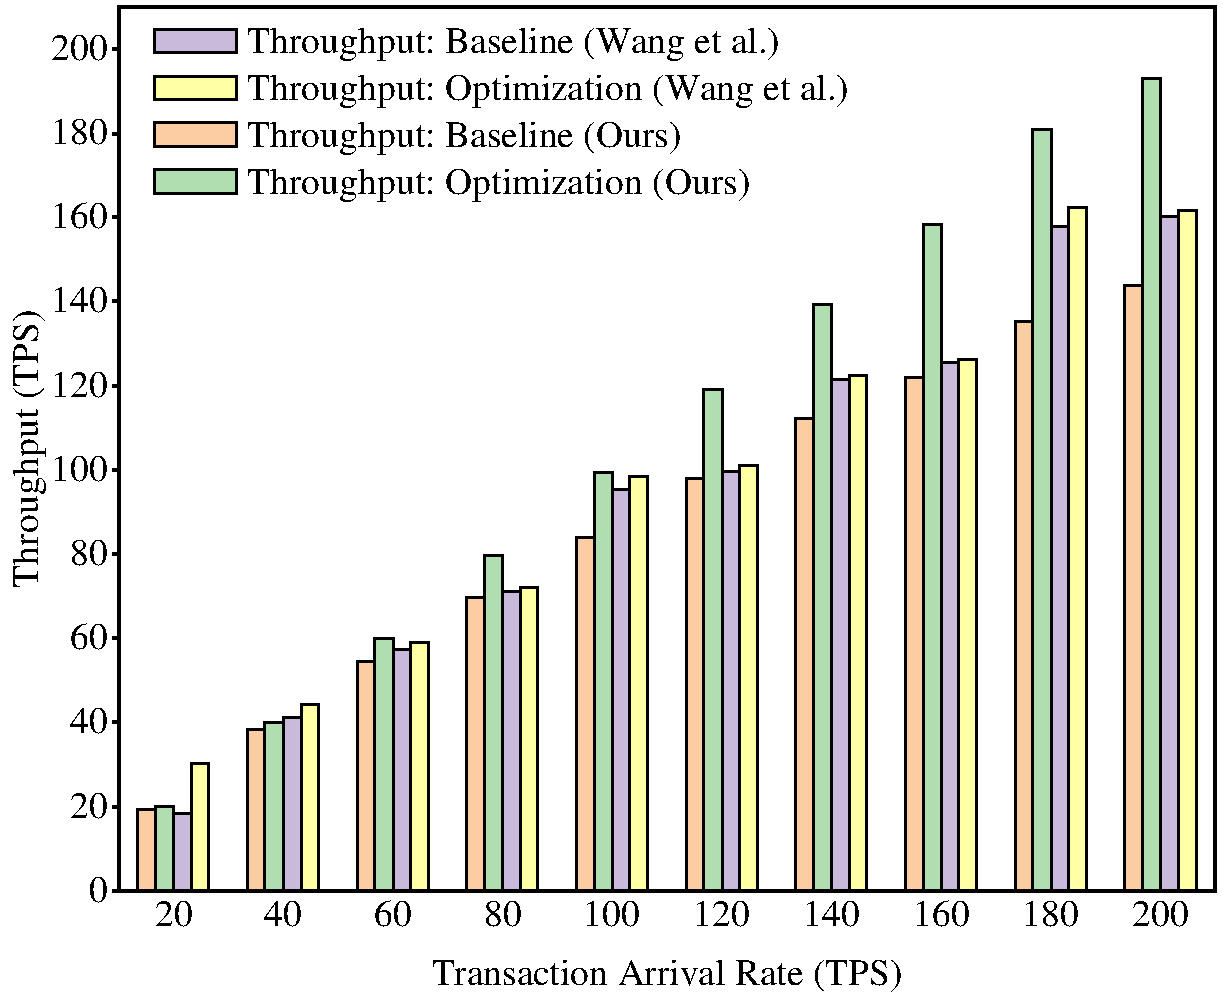
\includegraphics[width=.9\columnwidth]{figures/comparison_throughput.pdf}
	\caption{Throughput comparison under different TPS.}
	\label{fig:comparison_throughput}
\end{figure}
A similar trend can also be observed in terms of throughput. As the transaction arrival rate increases, DW-DQN maintains stable throughput growth while score-based strategies exhibit performance saturation. This indicates that the proposed optimization strategy can better exploit the available network resources by dynamically selecting appropriate block sizes. Consequently, the blockchain system is able to process more transactions without introducing excessive communication or confirmation delays.

The superior performance can be attributed to DW-DQN's ability to effectively model the nonlinear relationship among transaction load, block size, and system performance. Furthermore, the incorporation of experience replay and a discrete action space enhances training stability and facilitates smoother policy convergence, enabling the learned policy to generalize well under dynamic blockchain workloads. Overall, the experimental results demonstrate that the proposed optimization framework not only improves latency and throughput simultaneously, but also exhibits strong scalability and robustness under diverse transaction workloads, making it well suited for practical blockchain deployment scenarios.



\section{Conclusion}\label{sec:conclusion}

This paper introduces ChainOptNet, a comprehensive blockchain performance optimization framework that achieves significant system improvements by leveraging three key technical innovations. First, for transaction arrival rate prediction, we introduce the Convolutional Feature Aggregation and Distribution (CFAD) model, which leverages a novel deep learning architecture to effectively capture temporal dependencies and complex distributional patterns in transaction data. Second, in the domain of performance prediction, a multi-model collaborative framework is proposed to improve predictive accuracy and robustness by intelligently combining heterogeneous machine learning models. Third, the Dynamic Weight Deep Q-Network (DW-DQN) serves as the optimization mechanism, combining a DQN-based block-size controller with a trend-aware dynamic reward weighting module to support real-time adaptive block-size adjustment and balanced optimization across multiple objectives.

Extensive experimental evaluations demonstrate the effectiveness of the proposed framework. The results show that ChainOptNet improves latency reduction and throughput enhancement compared with representative forecasting, regression, ensemble-learning, fixed-configuration, and score-based optimization baselines, while maintaining high optimization efficiency across varying transaction loads. The framework has a high degree of generalization and adaptability, making it suitable for use in a wide range of dynamic blockchain environments.

Future research will investigate several promising directions to improve ChainOptNet's applicability and performance. These include: (1) lightweight optimization algorithms to reduce computational overhead, (2) extending the framework to support cross-chain performance optimization in heterogeneous public chain ecosystems, (3) designing scenario-specific optimization strategies tailored to particular application domains, (4) incorporating advanced security and privacy mechanisms during optimization processes, and (5) improving system adaptability. These future efforts are intended to accelerate the practical deployment of high-performance, intelligent blockchain infrastructure.















%

%\clearpage

% CRediT Authorship Contribution Statement
\section*{CRediT authorship contribution statement}
\addcontentsline{toc}{section}{CRediT authorship contribution statement}

Author 1: Conceptualization, Methodology, Writing -
final draft. Author 2: carrying out experiments and
Writing - original draft. The remaining authors contributed
to validating the ideas, carrying out additional analyses and
reviewing this paper. All authors read and approved the
manuscript.

% Data Availability
\section*{Data availability}
\addcontentsline{toc}{section}{Data availability}

Data will be made available on request.

% Declaration of Competing Interest
\section*{Declaration of competing interest}
\addcontentsline{toc}{section}{Declaration of competing interest}

The authors declare that they have no known competing financial interests or personal relationships that could have appeared to influence the work reported in this paper.

% Acknowledgements
\section*{Acknowledgements}
\addcontentsline{toc}{section}{Acknowledgements}
This work was supported by the ...
%Chongqing Research Program of Basic Research and Frontier Technology (Grant No. CSTB2025NSCQ-GPX1309).

\bibliographystyle{unsrtnat}
\bibliography{references}

\end{document}
